% Save this as tutorial.tex for the lwarp package tutorial.
\documentclass{book}
\usepackage{iftex}
% --- LOAD FONT SELECTION AND ENCODING BEFORE LOADING LWARP ---
\ifPDFTeX
\usepackage{lmodern} % pdflatex or dvi latex
\usepackage[T1]{fontenc}
\usepackage[utf8]{inputenc}
\else
\usepackage{fontspec} % XeLaTeX or LuaLaTeX
\fi
% --- LWARP IS LOADED NEXT ---
\usepackage[
HomeHTMLFilename=index, % Filename of the homepage.
% HTMLFilename={node-}, % Filename prefix of other pages.
% IndexLanguage=english, % Language for xindy index, glossary.
% latexmk, % Use latexmk to compile.
% OSWindows, % Force Windows. (Usually automatic.)
 mathjax, % Use MathJax to display math.
%mathsvg% Show math using SVG images.
GlossaryCmd={perl makeglossaries},
GlossaryCmd={makeglossaries -L english},
]{lwarp}
% \boolfalse{FileSectionNames} % If false, numbers the files.
% --- LOAD PDFLATEX MATH FONTS HERE ---
% --- OTHER PACKAGES ARE LOADED AFTER LWARP ---
\usepackage{calum_lecture} % My style file contains all of the packages, page, geometries, and custom commands that I like to use.
\makeglossaries
\usepackage{mat1001_glos}
\glstoctrue %Adds glossary to the table of contents

% --- LATEX AND HTML CUSTOMIZATION ---
%\title{MAT1001 Differential Calculus: Lecture Notes}
%\author{Calum Ross}
\setcounter{tocdepth}{2} % Include subsections in the \TOC.
\setcounter{secnumdepth}{2} % Number down to subsections.
\setcounter{FileDepth}{0} % Split \HTML\ files at sections
\booltrue{CombineHigherDepths} % Combine parts/chapters/sections
\setcounter{SideTOCDepth}{1} % Include subsections in the side\TOC
\HTMLTitle{MAT1001 Differential Calculus: Lecture Notes} % Overrides \title for the web page.
\HTMLAuthor{Calum Ross} % Sets the HTML meta author tag.
\HTMLLanguage{en-UK} % Sets the HTML meta language.
\HTMLDescription{Lecture notes for the module MAT1001 Differential Calculus.}% Sets the HTML meta description.
%\HTMLFirstPageTop{Name and \fbox{HOMEPAGE LOGO}}
%\HTMLPageTop{\fbox{LOGO}}
\HTMLPageBottom{Contact \href{mailto:rossc@edgehill.ac.uk}{rossc[at]edgehill[dot]ac[dot]uk} and Copyright CC BY 4.0}
%\CSSFilename{STM0005-physics.css} % This loads a css file that enables us to customise the webpage more. Currently I have not written a css file to be included here.

\MathJaxFilename{lwarp_mathjax.txt}

%%% Compact lists slightly less compact
%%\setlength{\plitemsep}{3pt}
\begin{document}
\pagenumbering{Alph} % to stop hyperref warnings
%\frontmatter
\title{MAT1001 Differential Calculus: Lecture Notes}
\author{Calum Ross}
\affiliation{Edge Hill University}
\date{Last modified: \today}
\maketitle % Or titlepage/titlingpage environment.
% An article abstract would go here.
\pagenumbering{roman}
\tableofcontents % MUST BE BEFORE THE FIRST SECTION BREAK!
%\listoffigures

\mainmatter

\chapter{Why Do We Need Calculus}
\label{sec:course intro}
%\pagenumbering{arabic}

\epigraph{\textbf{Calculus}: A branch of mathematics using the idea of a limit and generally divided into two parts: integral and differential calculus. }{\textit{Penguin Dictionary of Mathematics}}


\section{Course Overview}
\label{sec:overview}
These lecture notes cover the same material as the lectures for \textbf{MAT1001 Differential Calculus}. They will be updated during the module so please check back regularly for the latest version, the date of the most recent update is shown on the front page. In particular, most of the figures used in the lectures are hand drawn and it takes some time to produce good quality digital versions of these.\\

It is important to note that \textbf{reading these notes is not a substitute for attending the lectures and tutorials!} While I have included everything that I intend to cover in the lectures, and have often given more detail in these notes, the direction that we go in lectures will be guided by student questions and the example problems that you are given to solve. These are not reflected in the notes as I cannot anticipate all of the questions that may be asked. If you want to pass the module then the best way to do this is to attend the lectures and tutorials and to solve all of the practice problems that you are given.\\

In week one there was  overview information about the module including a rough schedule, how you will be assessed, and how to contact me. That will not be duplicated here and can be found on the module's virtual learning environment (VLE) page. If you need have any questions during the module then you can send me an \href{mailto:rossc@edgehill.ac.uk}{email} or come by my office during the office hour times. The module reading list, available on the VLE, contains details of recommended and supplementary reading for the module, there will frequently be suggested reading given to complement the material from a given weeks lecture. In these notes I will occasionally cite one of these books in the lecture notes, there will also be extra information and resources given in \cref{sec:further reading}. My favourite reference for much of this material is \citep{riley_mathematical_2006}, which covers all the areas of mathematics that we need for this course.\\

We will mainly be using content from chapters 1, 2, and parts of 27 from \citep{riley_mathematical_2006}.  Another good resource is the calculus page on the website \href{https://tutorial.math.lamar.edu/classes/calci/calci.aspx}{Paul's Online Notes}. There are lots of examples given there, some of which I have included in this lecture notes.\\

Another book that I have sometimes used is \citep{jordan2008mathematical}, it contains lots of background material but does not always have the simplest explanations. For numerical methods \citep{lissamen2004mei} contains a lot of material, and there are several copies in the library.\\


\section{Why Calculus}
\label{sec:why calculus}
\epigraph{\textbf{So what does calculus add for me?} It provides a way for us to construct relatively simple quantitative models of change, and to deduce their consequences. }{\textit{\href{https://math.mit.edu/~djk/calculus_beginners/chapter00/section02.html}{MIT Calculus for Beginners}}}

Calculus is an important topic in mathematics and at its most basic is the study of how functions change. It makes an appearance whenever we are interested in solving an optimisation problem, e.g. finding the best solution to a given problem. This could be finding out the largest area that can be enclosed by a fence of a given length, or what the fastest way to travel between two different points is. One example of this is sometimes called the \textbf{Ocado} or \textbf{vehicle routing problem} and wants to find the optimal route for a delivery van\footnote{More info on this can be found \href{https://www.cardiff.ac.uk/news/view/2585000-improving-vehicle-routing-with-ocado-group}{here}. Sometimes the Ocado problem refers to routing of the robots that pick up groceries in the warehouse which is another example of a vehicle routing problem.}. \\

\begin{figure}[ht]
    \centering
    %\pdftooltip{
    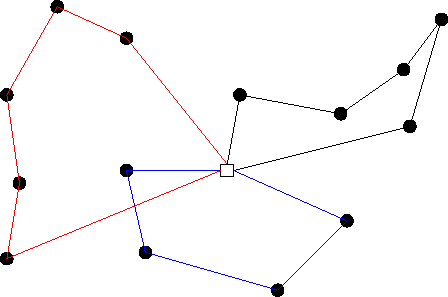
\includegraphics[width=0.35\textwidth, alt ={A schematic of the vehicle routing problem.}]{figures/vehicle_routing_problem}
    %}{. }
    \caption{A schematic of the vehicle routing problem. This is a programming problem where you want to find the optimal set of routes for a fleet of vehicles to travel when making deliveries to a given set of customers, the dots in the figure. This sort of optimisation problem is important for any delivery service as making their routes more efficient can save them money. }
\label{fig: vehicle routing}
\end{figure}

You may be thinking, ``that all sounds sensible in mathematics or physics, but as a computer science why should I care about calculus?'' If so you are not alone, many people ask the same question and there are many answers given online. For example the Medium post \href{https://medium.com/@18bhavyasharma/the-use-of-calculus-in-computer-science-a6917dbe33b9}{The uses of Calculus in Computer Science} highlights several areas:
\begin{itemize}
%\setlength{\itemsep}{-5pt}
    \item \textbf{Algorithms and optimisation:}  As highlighted above, whenever you have an optimisation problem calculus invariably rears its head.
    \item \textbf{Numerical analysis/ Computer graphics and computer vision:} Calculus provides a language for solving complex physical and mathematical problems that we are unable to solve by hand. This is important if you want to simulate a physical system, whether in a piece of scientific research or because you are designing a computer game, but also in graphics rendering and computer vision where you need to understand and simulate the path that light rays will follow.
   \item \textbf{AI and machine learning:} Most machine learning algorithms involve calculus in their optimisation and training.
   \item \textbf{Data science:} Much of data science involves statistical and mathematical modelling to analyse and understand the data. Understanding these techniques relies on understanding calculus. 
\end{itemize}
This all goes to show that calculus is an essential tool in many field beyond pure mathematics and is indispensable for Physicists, Engineers, and computer programmers. \\

\begin{figure}[ht]
    \centering
    %\pdftooltip{
    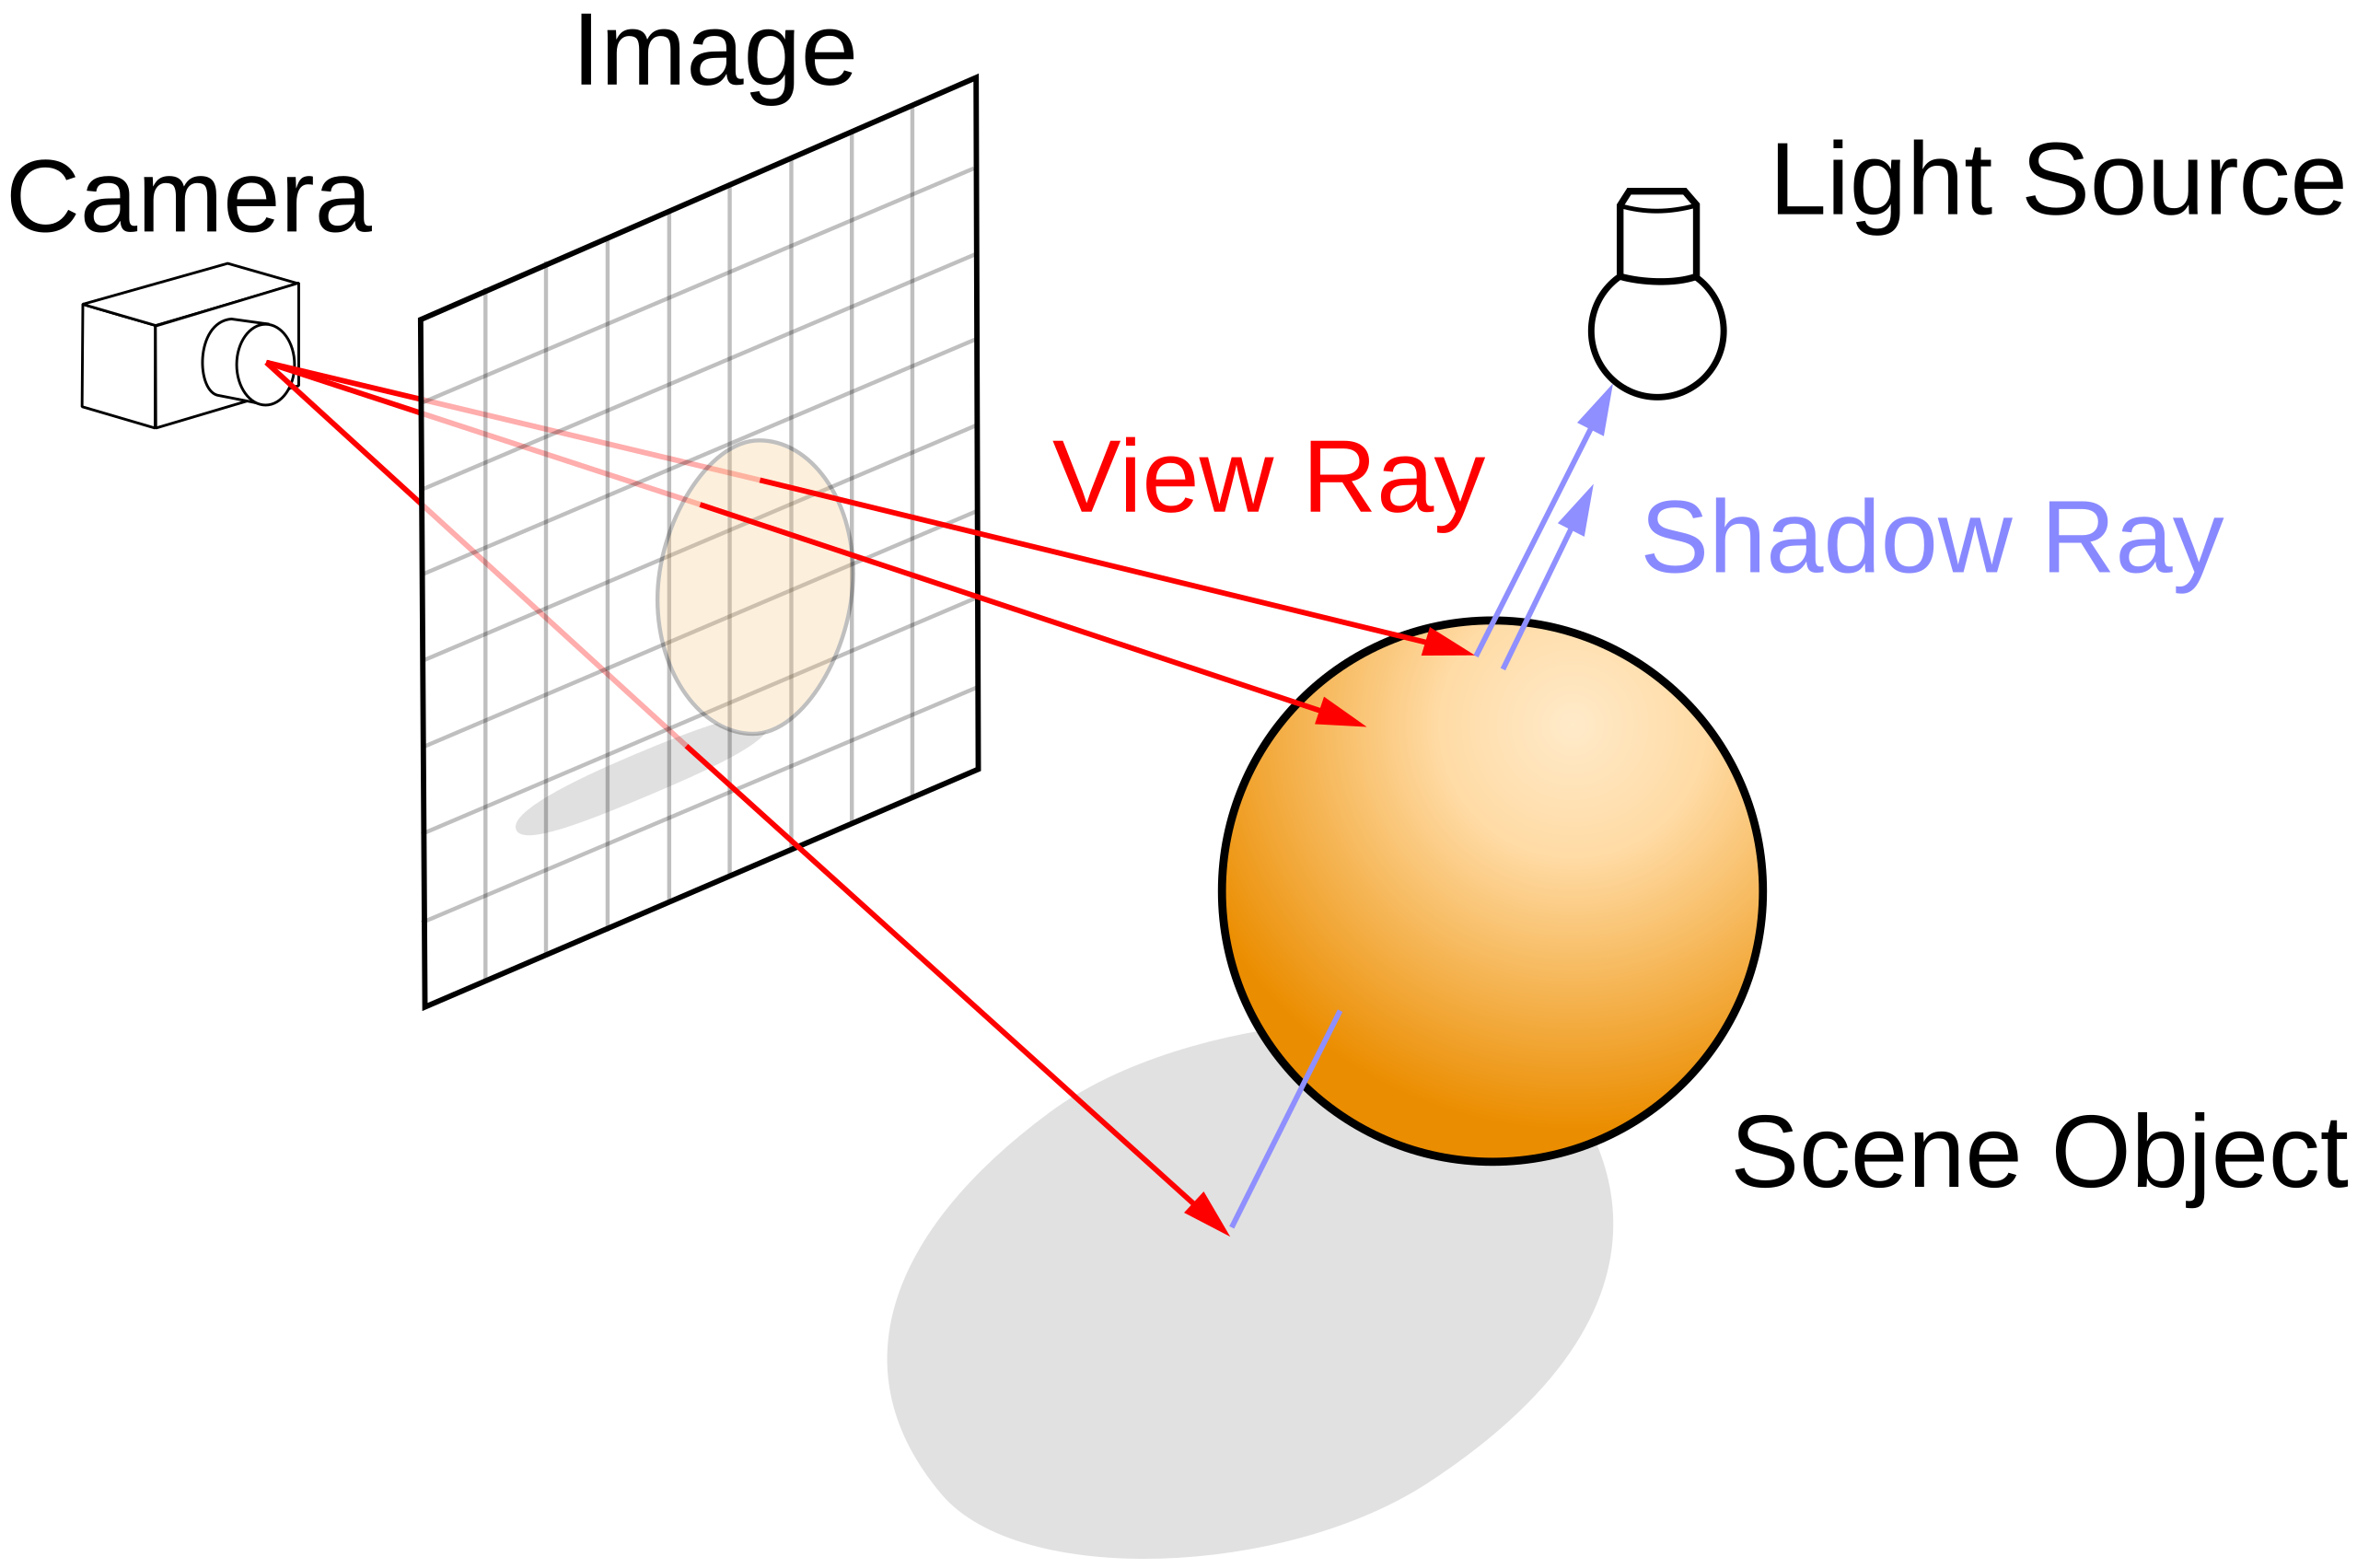
\includegraphics[width=0.6\textwidth, alt = {A schematic of ray tracing.}]{figures/Ray_trace_diagram}
    %}{A schematic of ray tracing. }
    \caption{A schematic showing how a ray tracung algorithm works to build up an image by extending light rays. This image was made by \href{https://commons.wikimedia.org/wiki/File:Ray\_trace\_diagram.svg}{Henrik} for Wikimedia Commons.}
\label{fig: ray tracing}
\end{figure}


Calculus is separated into two main areas: \textbf{\gls{Differentiation}} and \textbf{\gls{Integration}}. Differentiation is the study of how quickly or slowly a function varies. If we have a a graph of a function the derivative is the gradient to this graph, this notion will be made precise in a later section. Integration is the ``opposite'' of differentiation and corresponds to finding the area under the graph of a function.\\

Both concepts can be extended to much more abstract settings but the intuition gained from thinking about graphs of functions, their gradients, and the area under them, will set you in good stead for everything that comes after this.\\

\begin{figure}[ht]
    \centering
    %\pdftooltip{
    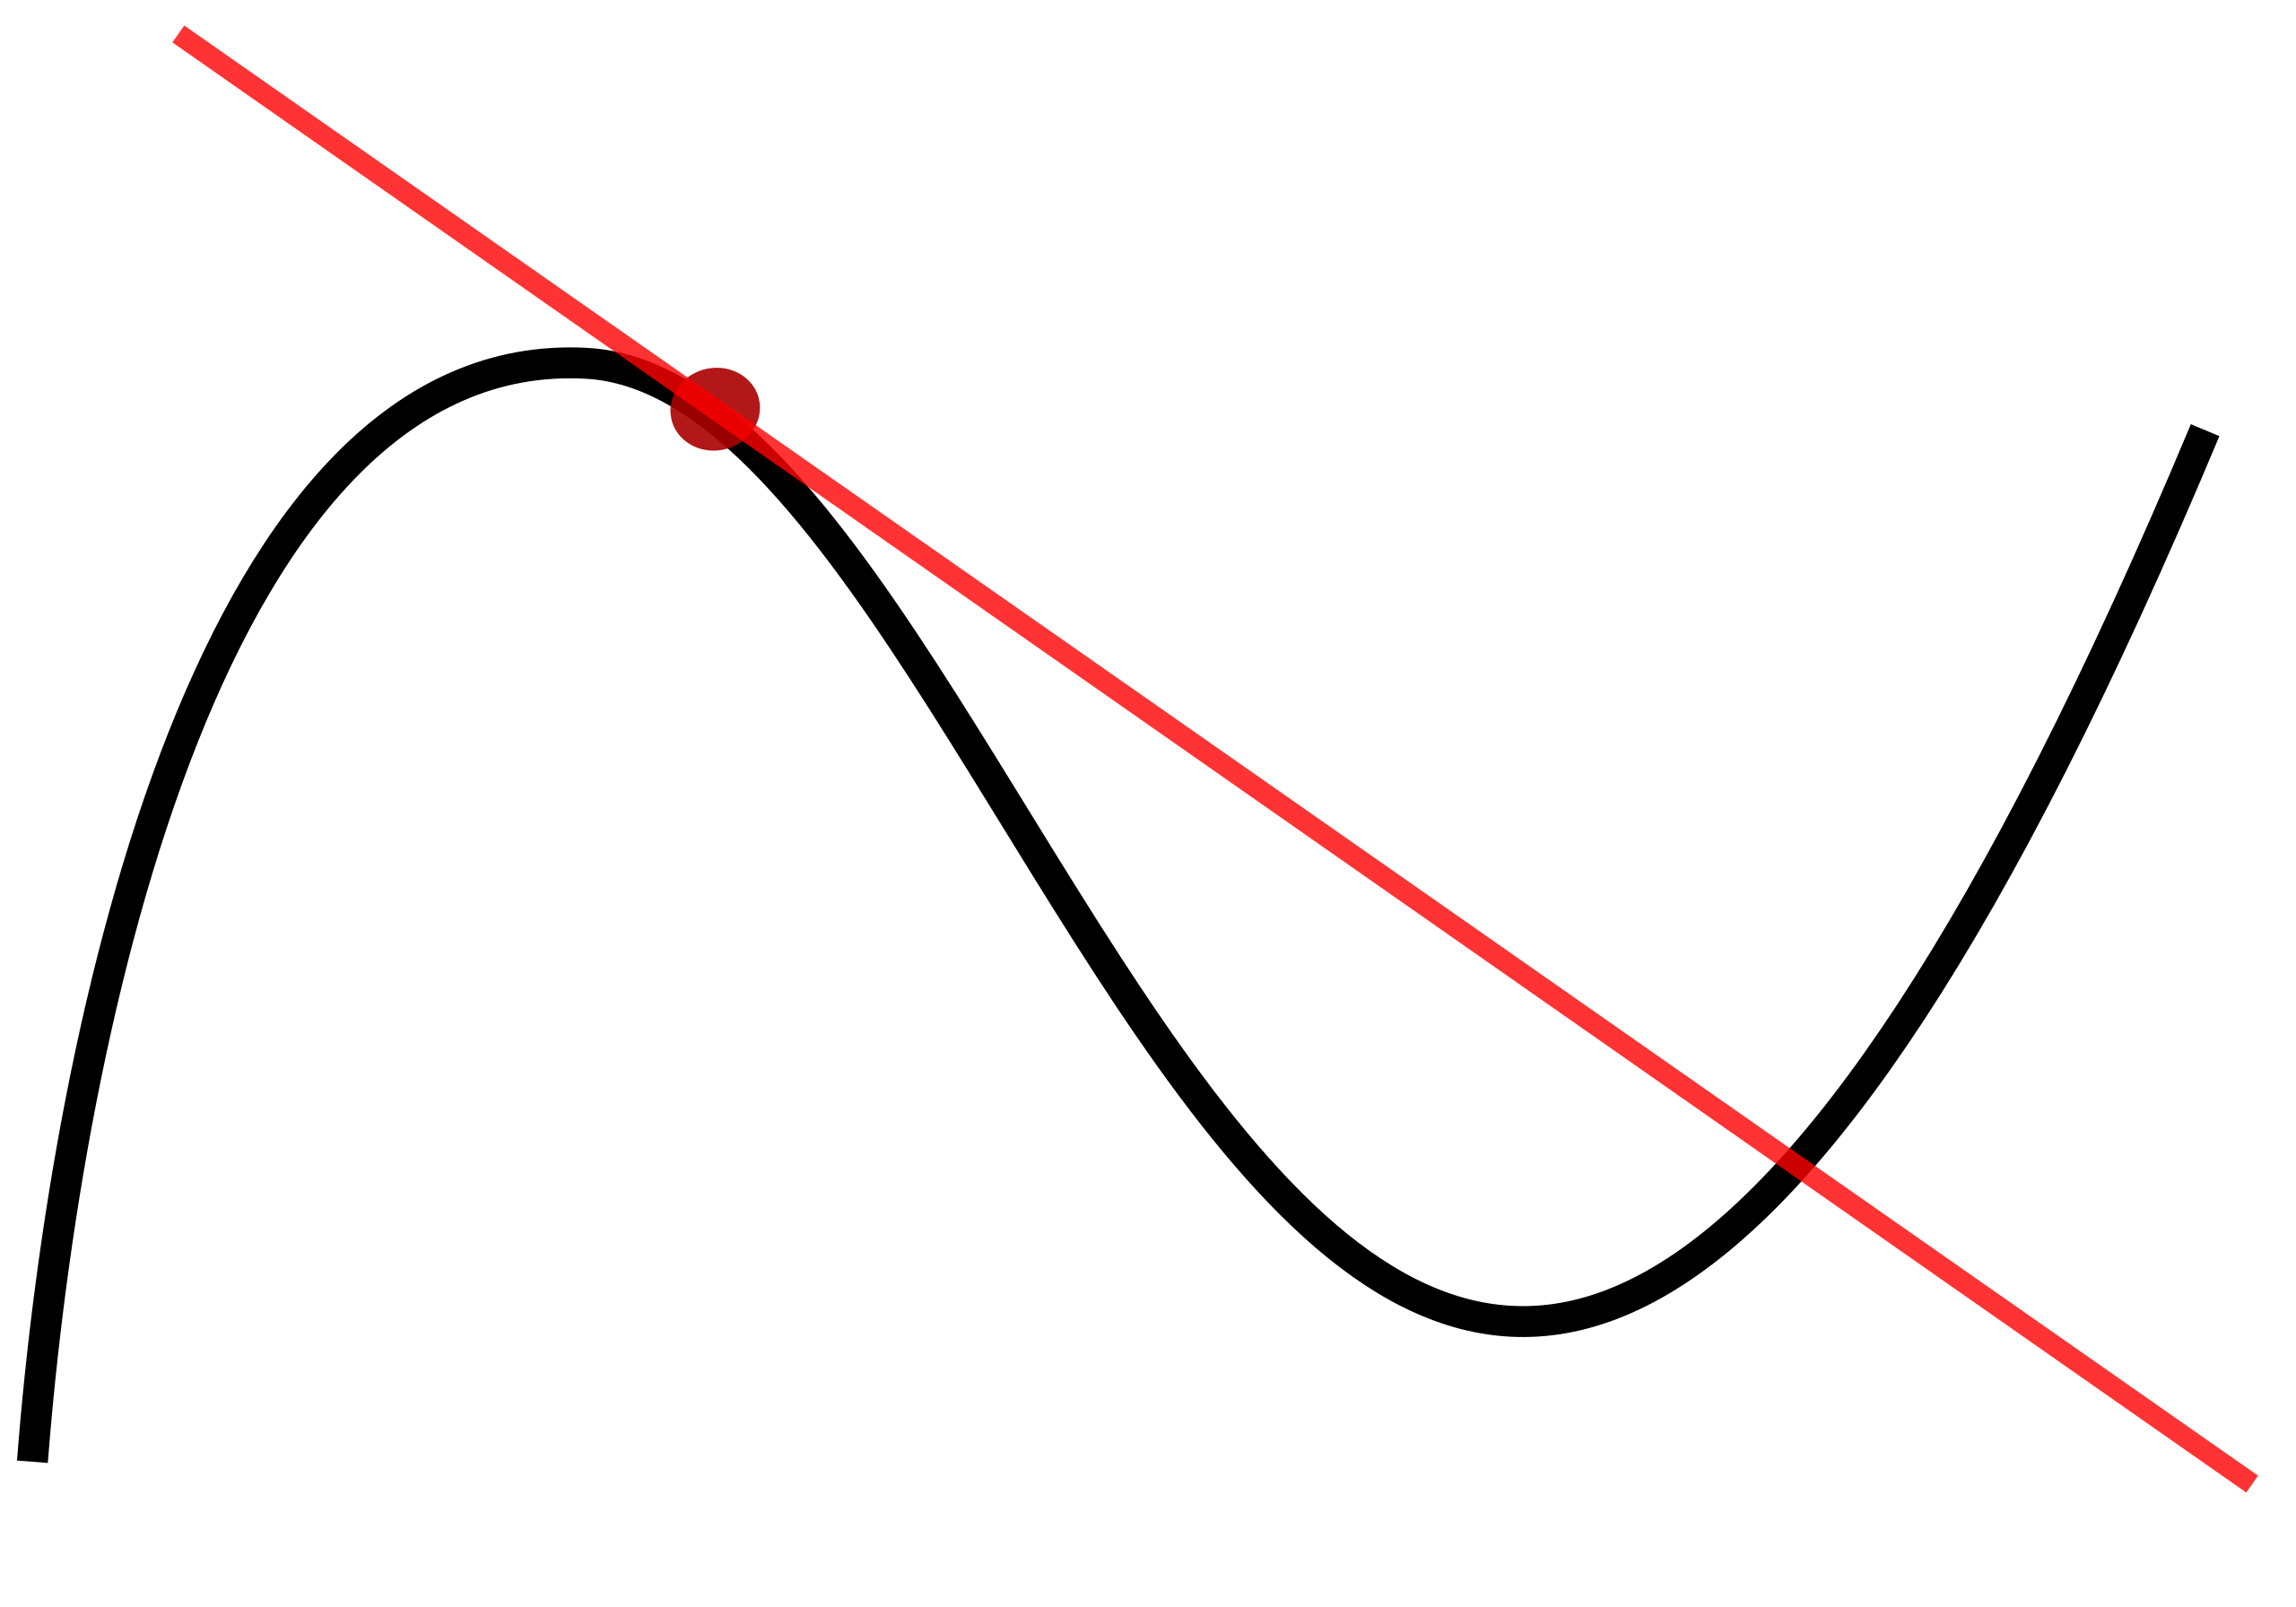
\includegraphics[width=0.3\textwidth, alt ={A schematic of the derivative as a tangent to a curve.}]{figures/Tangent_to_a_curve}
    %}{A schematic of a derivative as a tangent to a curve. }
    \caption{The derivative of a function at a point is equivalent to finding the tangent to a curve at this point.  }
\label{fig: derivative as tangent}
\end{figure}

\begin{figure}[ht]
    \centering
   % \pdftooltip{
   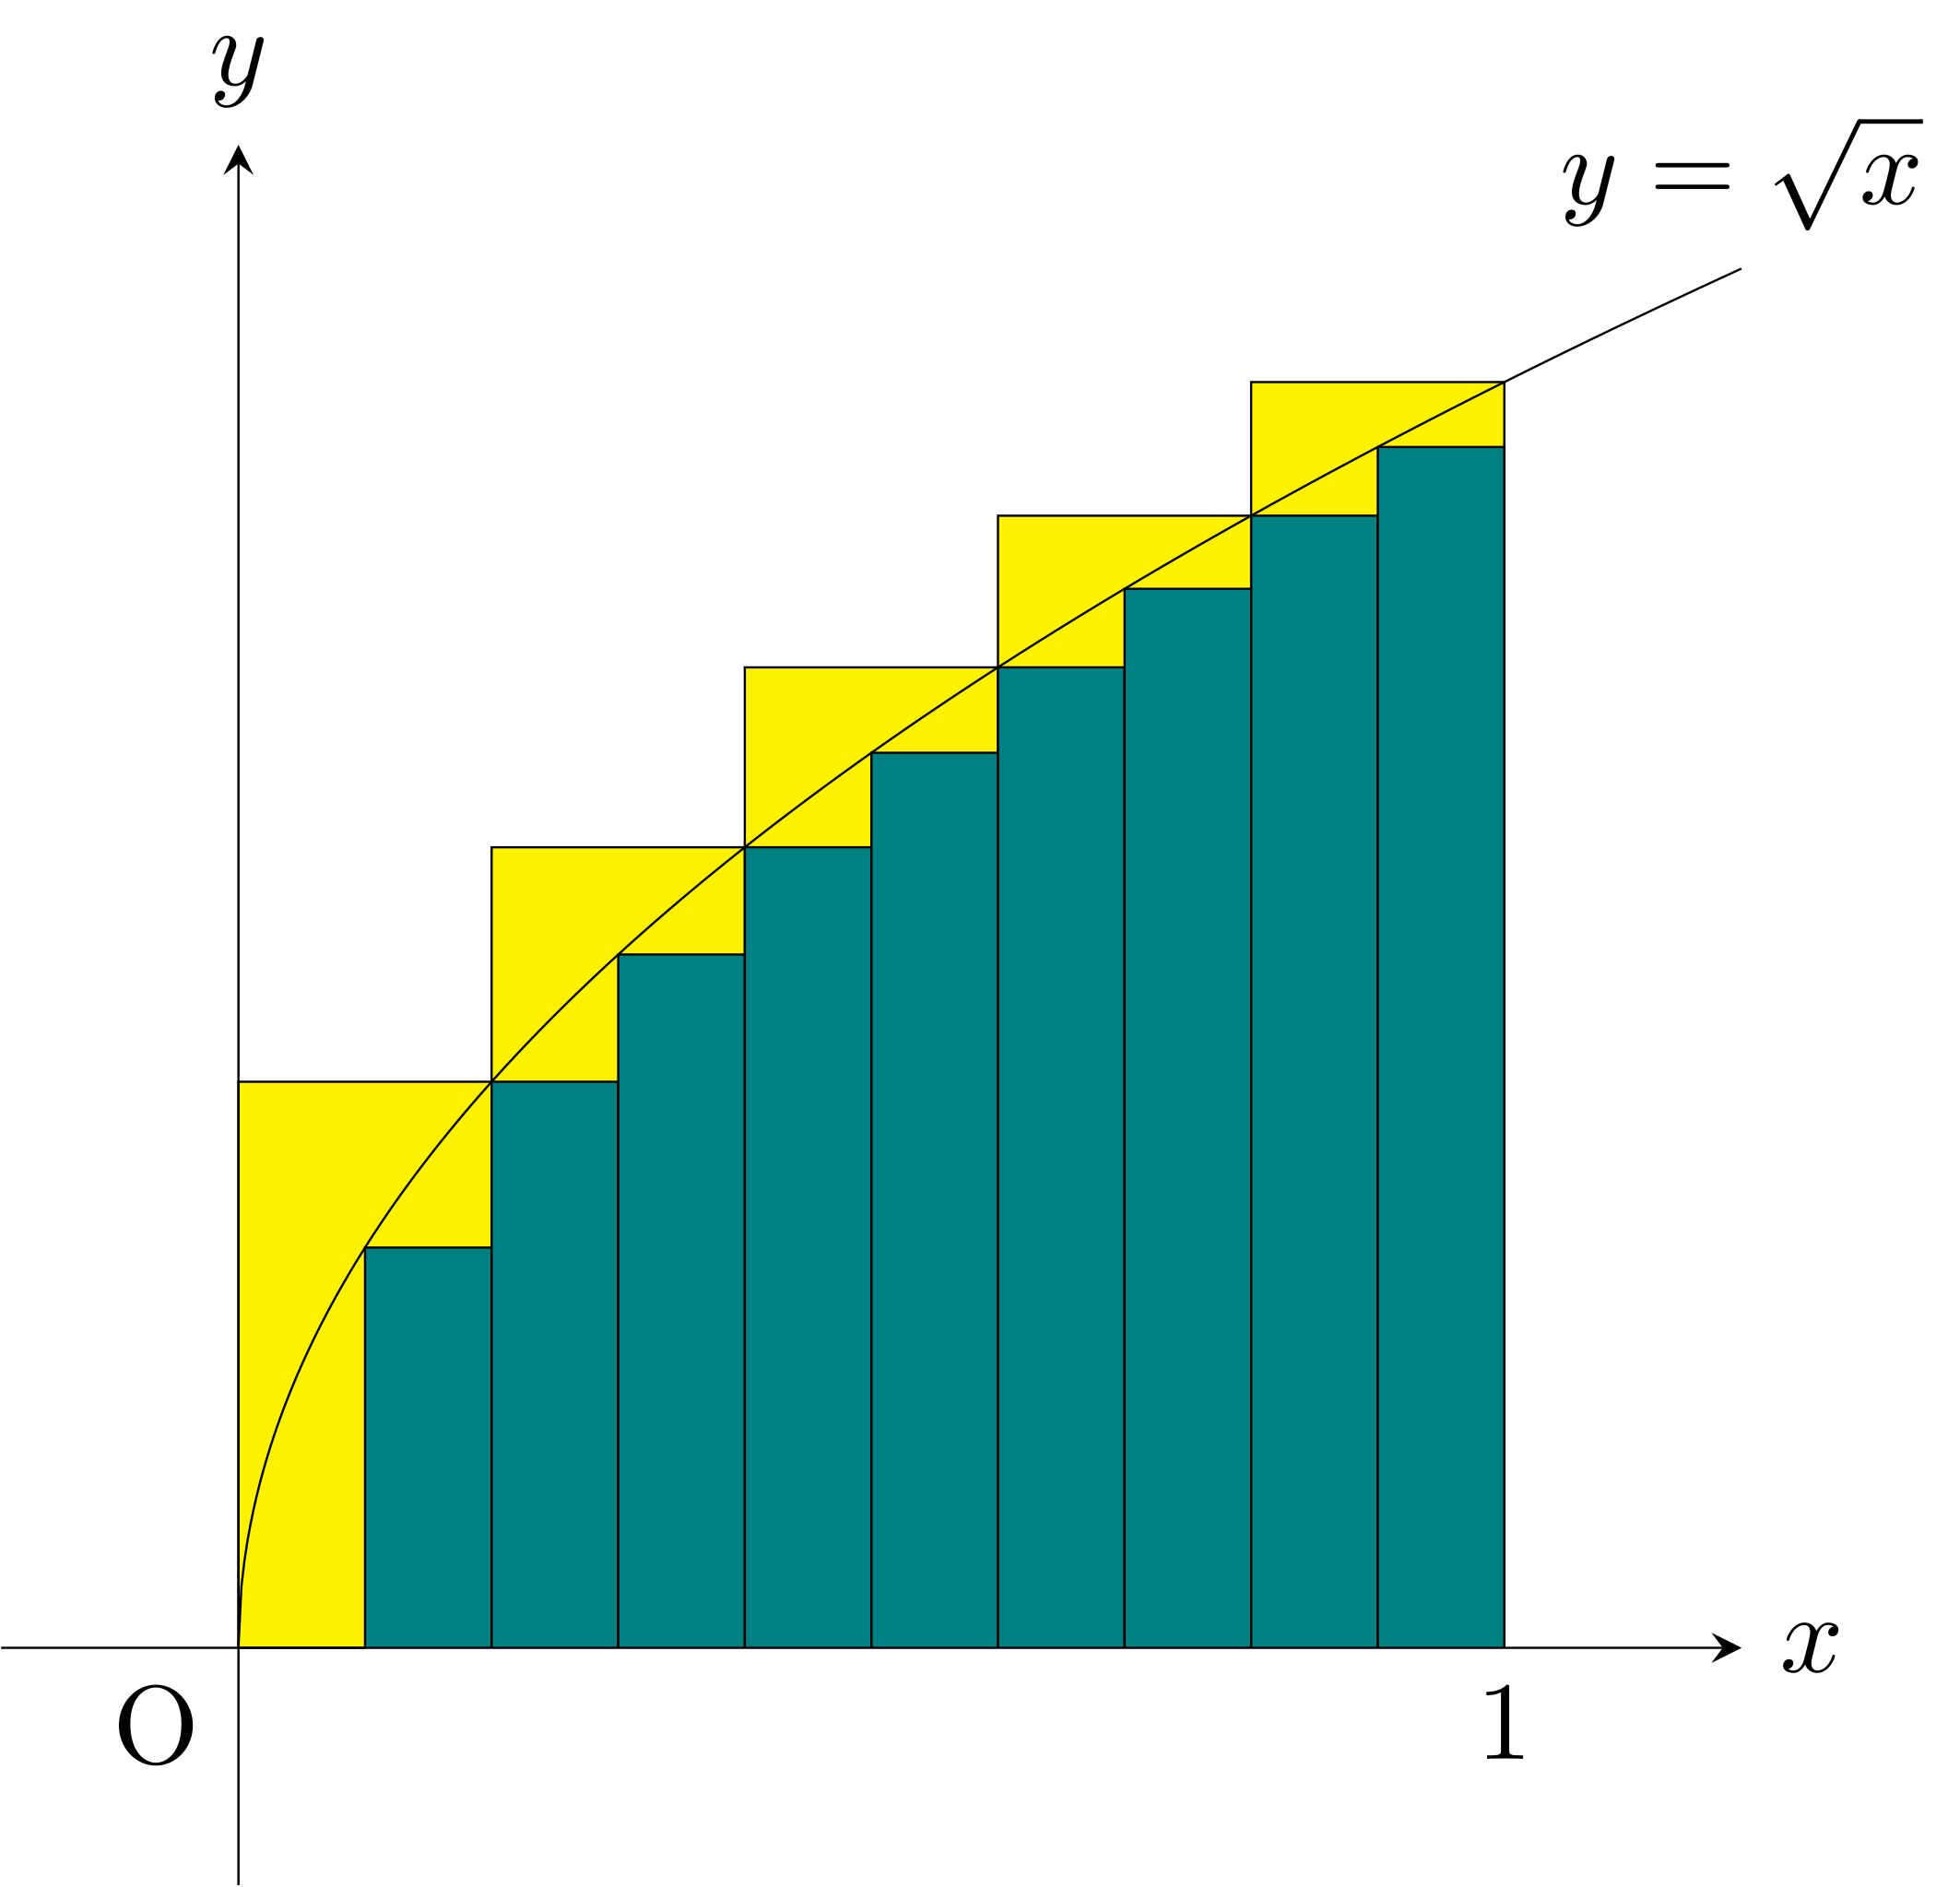
\includegraphics[width=0.4\textwidth, alt ={A schematic of an integral as the area under the curve.}]{figures/Integral_approximations}
   %}{A schematic of an integral as the area under the curve. }
    \caption{The integral, or area under the curve, can be approximated by rectangles. Depending on the size of the rectangles this can be an over estimate or an underestimate, but it will improve the thinner the rectangles become. This figure comes from \href{https://commons.wikimedia.org/wiki/File:Integral\_approximations\_J.svg}{Wikimedia Commons}. }
\label{fig: integral approximation}
\end{figure}
The YouTube channel 3Blue1Brown has an excellent playlist called the essence of calculus available \href{https://www.youtube.com/playlist?list=PLZHQObOWTQDMsr9K-rj53DwVRMYO3t5Yr}{here} which goes through the basics of calculus and its implications in a fairly unique way. Grant's goal in the videos is to give you an intuition for why Calculus works the way it does, rather than just giving you a list of facts and equations to memorise. Hopefully you will find that this module takes a similar approach, the goal is for you to understand the how and why of the mathematics and not just approach it as a set of rules to memorise. \\

If you find that you enjoy any of the topics in this module, or just want to read about interesting mathematics in a popular science setting I recommend having a look at \href{https://chalkdustmagazine.com/}{\textit{\gls{Chalkdust}} magazine}. As one of the editors of \textit{Chalkdust} I may be biased, but I think that it is a nice way to find out about some interesting maths without having to go into all of the details.\\

Hopefully, this has given you a feel for why you are doing this module. Now we can get started with the mathematics. As calculus is the study of how functions change we first need to remind ourselves of some of the properties of functions and introduce some notation.

\section*{How to use these notes }
As stated above, these notes are here to complement the in person lectures rather than to replace them.  For some topics there will be more detail given here, while at other points there may be explanations that I give in the lectures, or examples that I use which do not appear in these notes.  Also, I will frequently draw pictures in the lectures, as the module goes on I will try to add these figures to the lecture notes. However, that will not always be possible. These notes also contain exercises, some of which will appear in the tutorial sheets, that you should solve to help reinforce the concepts from the module.\\

To complement the theory presented in these notes you will find a range to examples and exercises to help you build familiarity with the mathematical concepts that we will meet during this module. As this is not a module for mathematicians we will not always completely precise and give all the details, but rather focus on the practical applications of the mathematics. Occasionally I will include a \textbf{\gls{Mathematical Diversion}} where I give some more of these details. If you are interested in the mathematics for its own sake then these will hopefully be interesting to you. If you are only interested in the mathematics that you need to pass this module, then feel free to skip these diversions.\\

\begin{warpprint} % For print only output ...
These lecture notes will continue to develop as the module goes on so make sure to check back frequently to see what has been added. There is also an online html version of these notes that you can check out as well. The html version should be accessible with alttext on the figures. If you have any difficulty viewing either these notes or the html version let me know.
\end{warpprint}


\newpage

%%%%%%%%%%%%%%%%%%%%%%%%%%%%%%%%%%%%%%%%%%%%%%

\chapter{Functions}
\label{sec:functions}

\epigraph{The art of doing mathematics is finding that special case that contains all the germs of generality. }{\textit{David Hilbert}}

\section{What is a function}
The concept of a function is essential to understand not just calculus but also computer programming. We can think of a function as being a black box that takes in information, potentially changes it in some way, and then outputs information.\\

\begin{figure}[ht]
    \centering
    %\pdftooltip{
    
\includegraphics[width=0.3\textwidth, alt ={A schematic of how a function behaves produced by Bin Im Garten for Wikimedia Commons.}]{figures/Injection_keine_Injektion_2a.png}
    %}{A schematic of how a function behaves produced by \href{Bin Im Garten} for Wikimedia Commons. }
    \caption{A schematic of how a function behaves, it maps objects $1,2,3,\dots$ in the \gls{set} $X$ to objects $A,B,C,D,\dots$ in the set $Y$. This image was produced by \href{https://commons.wikimedia.org/wiki/File:Injection\_keine\_Injektion\_2a.svg}{Bin Im Garten} for Wikimedia Commons.}
\label{fig: function schematic}
\end{figure}

Being more precise, a function is a map between two spaces, the domain, and the codomain. e.g.
\begin{equation*}
f:X\to Y
\end{equation*}
and it sends a point $x\in X$ to a point $f(x)=y\in Y$.  Functions have the property that they map a point $x\in X$ to a single point $y\in Y$,for example:
\begin{equation*}
y=f(x)=x^{2}+1,
\end{equation*}
is a function since every value of $x$ gives a single value of $y$. However, 
\begin{equation*}
y^{2}=x+1,
\end{equation*}
is not a function since every $x$ corresponds to two values of $y$, e.g. if $x=3$ then $y^{2}=3+1=4$ and $y$ can be both $2$ and $-2$.\\

Note that when we write $f(x)$ we are not saying $f$ times $x$, but mean that $f$ is a function of $x$, e.g. $f$ takes in a value of $x$ and returns a number $y=f(x)$.\\

Throughout this module we will meet several different types of functions so you will need to get familiar with this notation and understand how to evaluate functions. There will be some questions in the tutorial sheet to help you practice this.\\

A key property of a function is its \textbf{\gls{roots}} or zeros, these are the values of $x$ such that $f(x)=0$. For linear functions finding the roots is just a matter of rearranging the equation, sometimes referred to as changing the subject. In this module I am assuming that you have some familiarity with this, if not take a look at the background material in \cref{sec:background} or ask me to point you towards more resources. There will also be some revision questions on this topic in the first couple of weeks tutorials.

\begin{ex} Find all the roots of $f(x)=9x^{3}-18x^{2}+6x$.\\

Remember the roots are where $f(x)=0$ so we are solving $9x^{3}-18x^{2}+6x=0$. First notice that there is a common factor of $3x$ in all of the terms so we can factor that out and get
\begin{equation*}
0=9x^{3}-18x^{2}+6x=3x\left(3x^{2}-6x+2\right).
\end{equation*}
This means that either $x$ is zero or the quadratic expression in brackets, $3x^{2}-6x+2$, is zero. This means that $x=0$ is a root of the equation, and there will be two more that we find by solving the quadratic. This can be done by using the quadratic formula:
\begin{align*}
x&=\frac{6\pm\sqrt{(-6)^{2}-4(3)(2)}}{2(3)}\\
&=\frac{6\pm\sqrt{12}}{6}\\
&=1\pm\frac{\sqrt{3}}{3}\\
&=1\pm\frac{1}{\sqrt{3}}.
\end{align*}

So the three roots of $f(x)$ are
\begin{equation*}
x=0,\quad x=1+\frac{\sqrt{3}}{3},\quad x=1-\frac{\sqrt{3}}{3}.
\end{equation*}

\end{ex}

If you do not remember how to use the quadratic formula then I suggest that you look at the background material in \cref{sec:background}.\\

If this was a course for mathematicians this is where we would spend time talking about the domain and range of a function. How they are defined, and when we need to be careful to avoid dividing by zero. Here, we will not go through this, and I will just remind you that in your algebraic manipulations you should not divide by any quantity that is zero.\\

A simple, yet useful, class of functions are the rational functions. There are functions who are the ratio of two polynomials, e.g. 
\begin{equation*}
f(x)=\frac{4x+10}{x^{2}-2x-15}.
\end{equation*}

A useful way to understand a function is draw a graph. In a graph, the domain of the function $X$ is drawn horizontally and the codomain, $Y$, is drawn vertically, using \textbf{\gls{Cartesian} axes} $(x,y)$. The graph consists of the points $(x,y)$ with $y=f(x)$. In many books $x$ is called the independent variable and $y$ the dependent variable. In the tutorials we will discuss how to produce plots using a computer, either using \textbf{MATLAB}, \textbf{Python}, or \href{https://www.wolframalpha.com/}{\textbf{WolframAlpha}}. There are also online graphing programs like \href{https://www.desmos.com/}{\textbf{desmos}} and \href{https://www.geogebra.org/}{\textbf{GeoGebra}}. In these notes most of the graphs are produced using the Tikz package for \LaTeX{}, which is a typesetting and markup language\footnote{If you want to produce professional looking documents which include mathematical formulas then it is worth your time learning how to use \LaTeX{}.}.

\begin{ex}
Plot the graph of $f(x)=2x^{2}-1$.\\
\begin{figure}[htbp]
    \begin{center}
\ThisAltText{Graph of a quadratic.}
   % \pdftooltip{
    \begin{tikzpicture}[line width=1pt,line cap=round,line join=round,domain=-1:1, smooth,variable=\x,scale=2]
     \draw[->] (-1.2,0) -- (1.2,0) node[above] {$x$};
  \draw[->] (0,-1.2) -- (0,1.2) node[above] {$y$};
 \draw[color=red]   plot (\x,{2*\x*\x -1}) node[right] {$f(x)=2x^{2}-1$};
    \end{tikzpicture}
%    }{graph of a quadratic}
    \caption{The graph of the quadratic function  $f(x)=2x^{2}-1$ is a parabola which intersects the $y$-axis at $x=0$ and the $x$-axis at $x=\pm\frac{1}{\sqrt{2}}$.}
        \label{fig: quadratic function graph}
\end{center}
\end{figure}
\end{ex}
Note that the equation $y^{2}=x+1$ also defines a parabola, see \cref{fig: non equation}. However if we plot this function the curve is not the graph of a function. You should think about why this is.

\begin{figure}[ht]
    \centering
    %\pdftooltip{
    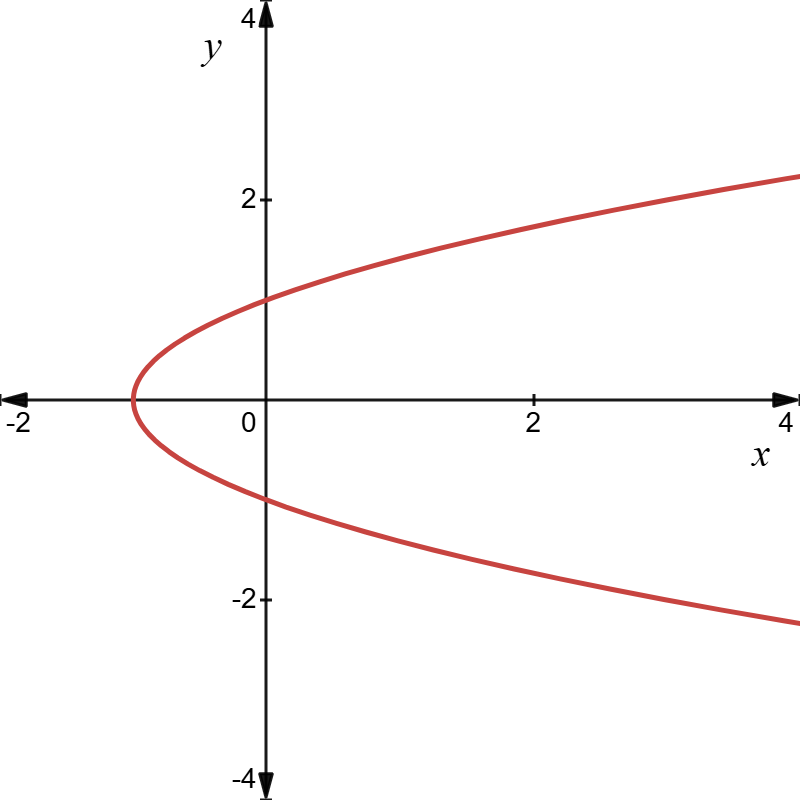
\includegraphics[width=0.4\textwidth, alt={An equation which does not give a graph.}]{figures/desmos-graph_non-function}
    %}{An equation which does not give a graph. }
    \caption{A plot of $y^{2}=x+1$, you should think about why this is not the graph of a function. }
\label{fig: non equation}
\end{figure}

\begin{ex}The function $f(x)=\sin(x)$ has the graph shown in \cref{fig: sine function graph}.\\
\begin{figure}[htbp]
    \centering
\ThisAltText{graph of sin(x).}
  %  \pdftooltip{
    \begin{tikzpicture}[line width=1pt,line cap=round,line join=round,domain=-6.282:6.282, smooth,variable=\x]
     \draw[->] (-6.282,0) -- (6.282,0)node[above] {$x$};
  \draw[->] (0,-1.2) -- (0,1.2) node[above] {$y$};
 \draw[color=CDred]   plot (\x,{sin(\x r)}) node[right] {$f(x)=\sin(x)$};
    \end{tikzpicture}
  %  }{graph of sin}
    \caption{The graph of the sine function  $f(x)=\sin(x)$.}
        \label{fig: sine function graph}
\end{figure}
\end{ex}

\begin{ex}
Consider the two functions $f(x)=3x-2$ and $g(x)=x/3 +2/3$. These satisfy the relationship
\begin{align*}
\left(f\circ g\right)(x)	&=f\left(g(x)\right)\\
				&=f\left(\frac{x}{3}+\frac{2}{3}\right)\\
				&=3\left(\frac{x}{3}+\frac{2}{3}\right)-2\\
				&=x+2-2=x
\end{align*}
and 
\begin{align*}
\left(g\circ f\right)(x)=x.
\end{align*}

When we have two functions whose composition leaves $x$ unchanged, we say that they are \textbf{\gls{inverse}} to each other, and $g$ is the inverse\footnote{Usually the inverse function is denoted as $f^{-1}$, though we need to be careful to understand that this does not mean $1/f$.} of $f$. As can be seen in Section 1.2 of \citep{calcI} we can understand this a meaning that if $f:x\mapsto y$ then $g:y\mapsto x$, e.g. $f(-1)=-5$ while $g(-5)=-1$.
\end{ex}

The concept of an inverse function makes intuitive sense. However, if we pretend to be mathematicians and treat this carefully we quickly encounter some problems. For example, what happens if we have a function which sends two different values of $x$ to the same value? Then we are unable to know which value we started with, so cannot build an inverse function. For example $f(x)=x^{2}$ sends both $x$ and $-x$ to $x^{2}$ so we cannot find an inverse that works everywhere, this is why when we firts meet the square root function you often see it as $\pm\sqrt{\phantom{+}}$.\\

Mathematicians fix this by introducing the notion of a \textbf{\gls{one-to-one}} function, sometimes called an \textbf{injective} function. A function is called one-to-one if no two values of $x$ produce the same value of $y$, so that
\begin{equation*}
f(x_{1})\neq f(x_{2}) \qquad \text{ for } x_{1}\neq x_{2}.
\end{equation*}

The advantage of one-to-one functions is that we can find inverses for them. If we have two one-to-one functions which satisfy 
\begin{equation*}
\left(f\circ g\right)(x)=x=\left(g\circ f\right)(x),
\end{equation*}
then $f$ and $g$ are inverses and we write $g(x)=f^{-1}(x)$.

\section{Trigonometric functions}
\label{sec: trig func}

Now that we have discussed functions and how to graph them, we can focus on some specific functions which it is very common to encounter.\\ 

From your previous maths experience you have probably come across \textbf{\gls{trigonometric}} (trig) functions in the context of triangles, where they are used to calculate lengths and angles. If you do not remember how this works then I suggest that you have a look at the Triganometry primer in \cref{sec:background} or check out some revision material available \href{https://corbettmaths.com/2013/03/30/trigonometry-introduction/}{here}. Another important thing to remember is that you should always work in radians rather than degrees when using trig functions. This is because radians are a more natural unit for angles and if we did not use them lots of formulas would need extra factors of $\uppi$ to be added for them to be valid. \\

\begin{figure}[ht]
    \centering
\ThisAltText{Converting from a circle to trig functions.}
  %  \pdftooltip{
    \begin{tikzpicture}[line width=1pt,line cap=round,line join=round, scale = 1.5]
   % \draw[step=1cm,gray,very thin] (3,-3) grid (3,3);
   \draw[->,ultra thick] (0,-2.4)--(0,2.4);
     \draw[->,ultra thick] (-2.4,0)--(2.4,0);
   \filldraw[color = blue, ultra thick](0,0) circle (0.05);
    \draw[ ultra thick](0,0) circle (2);
    \draw[ultra thick] (0,0) -- (2,0);
    \draw[ultra thick] (1,0) arc (0:45:1) node[anchor=north]{$\ut$};
     %\draw[ultra thick, color=red] (2,0) arc (0:45:2) node[anchor=north]{$s$};
     \draw[color = blue, ultra thick](0,0)--node[anchor=south]{$r$}(1.414,1.414) ;
     \draw[dashed, ultra thick] (0,1.414)node[left]{$\sin\ut$} --(1.414,1.414);
      \draw[dashed, ultra thick] (1.414,0) node[below]{$r\cos\ut$}--(1.414,1.414);
    \end{tikzpicture}
 %   }{Converting from a circle to trig functions}
    \caption{Trig functions and their relationship to a unit circle, this is true whatever the angle $\ut$ is, though we need to be careful about the signs of $x$ and $y$ }
        \label{fig:trig and circles}
\end{figure}


In the setting of triangles the angles are restricted to run between $0$ and $\uppi$ radians as for angles greater than this we would no longer have a triangle. However, the functions are valid for any real values of the argument, $x$. Typically we will be interested in angles within the range $[0,2\uppi)$, but need to remember that, as shown in \cref{fig: trig functions}, these functions are $2\uppi$ periodic. This means that
\begin{align*}
\sin(x+2\uppi)=\sin(x),\\
\cos(x+2\uppi)=\cos(x),\\
\tan(x+2\uppi)=\tan(x).
\end{align*}

We can think of these as functions from $[0,2\uppi)\to [-1,1]$ which reduce to the familar trig functions for angles between $0$ and $\uppi$.\\

\begin{figure}[ht]
    \centering
\ThisAltText{Graph of sin(x) and cos(x).}
   % \pdftooltip{
    \begin{tikzpicture}[line width=1pt,line cap=round,line join=round,domain=-6.28:6.28, smooth,variable=\x]
     \draw[->] (-7,0) -- (7,0) node[above] {$x$};
  \draw[->] (0,-1.3) -- (0,1.3);
 \draw[color=CDnavy]   plot[samples=300] (\x,{cos(\x r)}) node[right] {$\cos(x)$};
  \draw[color=CDgreen, dashed]   plot[samples=300] (\x,{sin(\x r)}) node[anchor = north west] {$\sin(x)$};
    \end{tikzpicture}
 %   }{plots of sin and cos }
    \caption{Plots of the trig functions $\sin(x)$ and $\cos(x)$ for $x$ between $-2\uppi$ and $2\uppi$.}
        \label{fig: trig functions}
\end{figure}


\begin{figure}[ht]
    \centering
  %  \pdftooltip{
  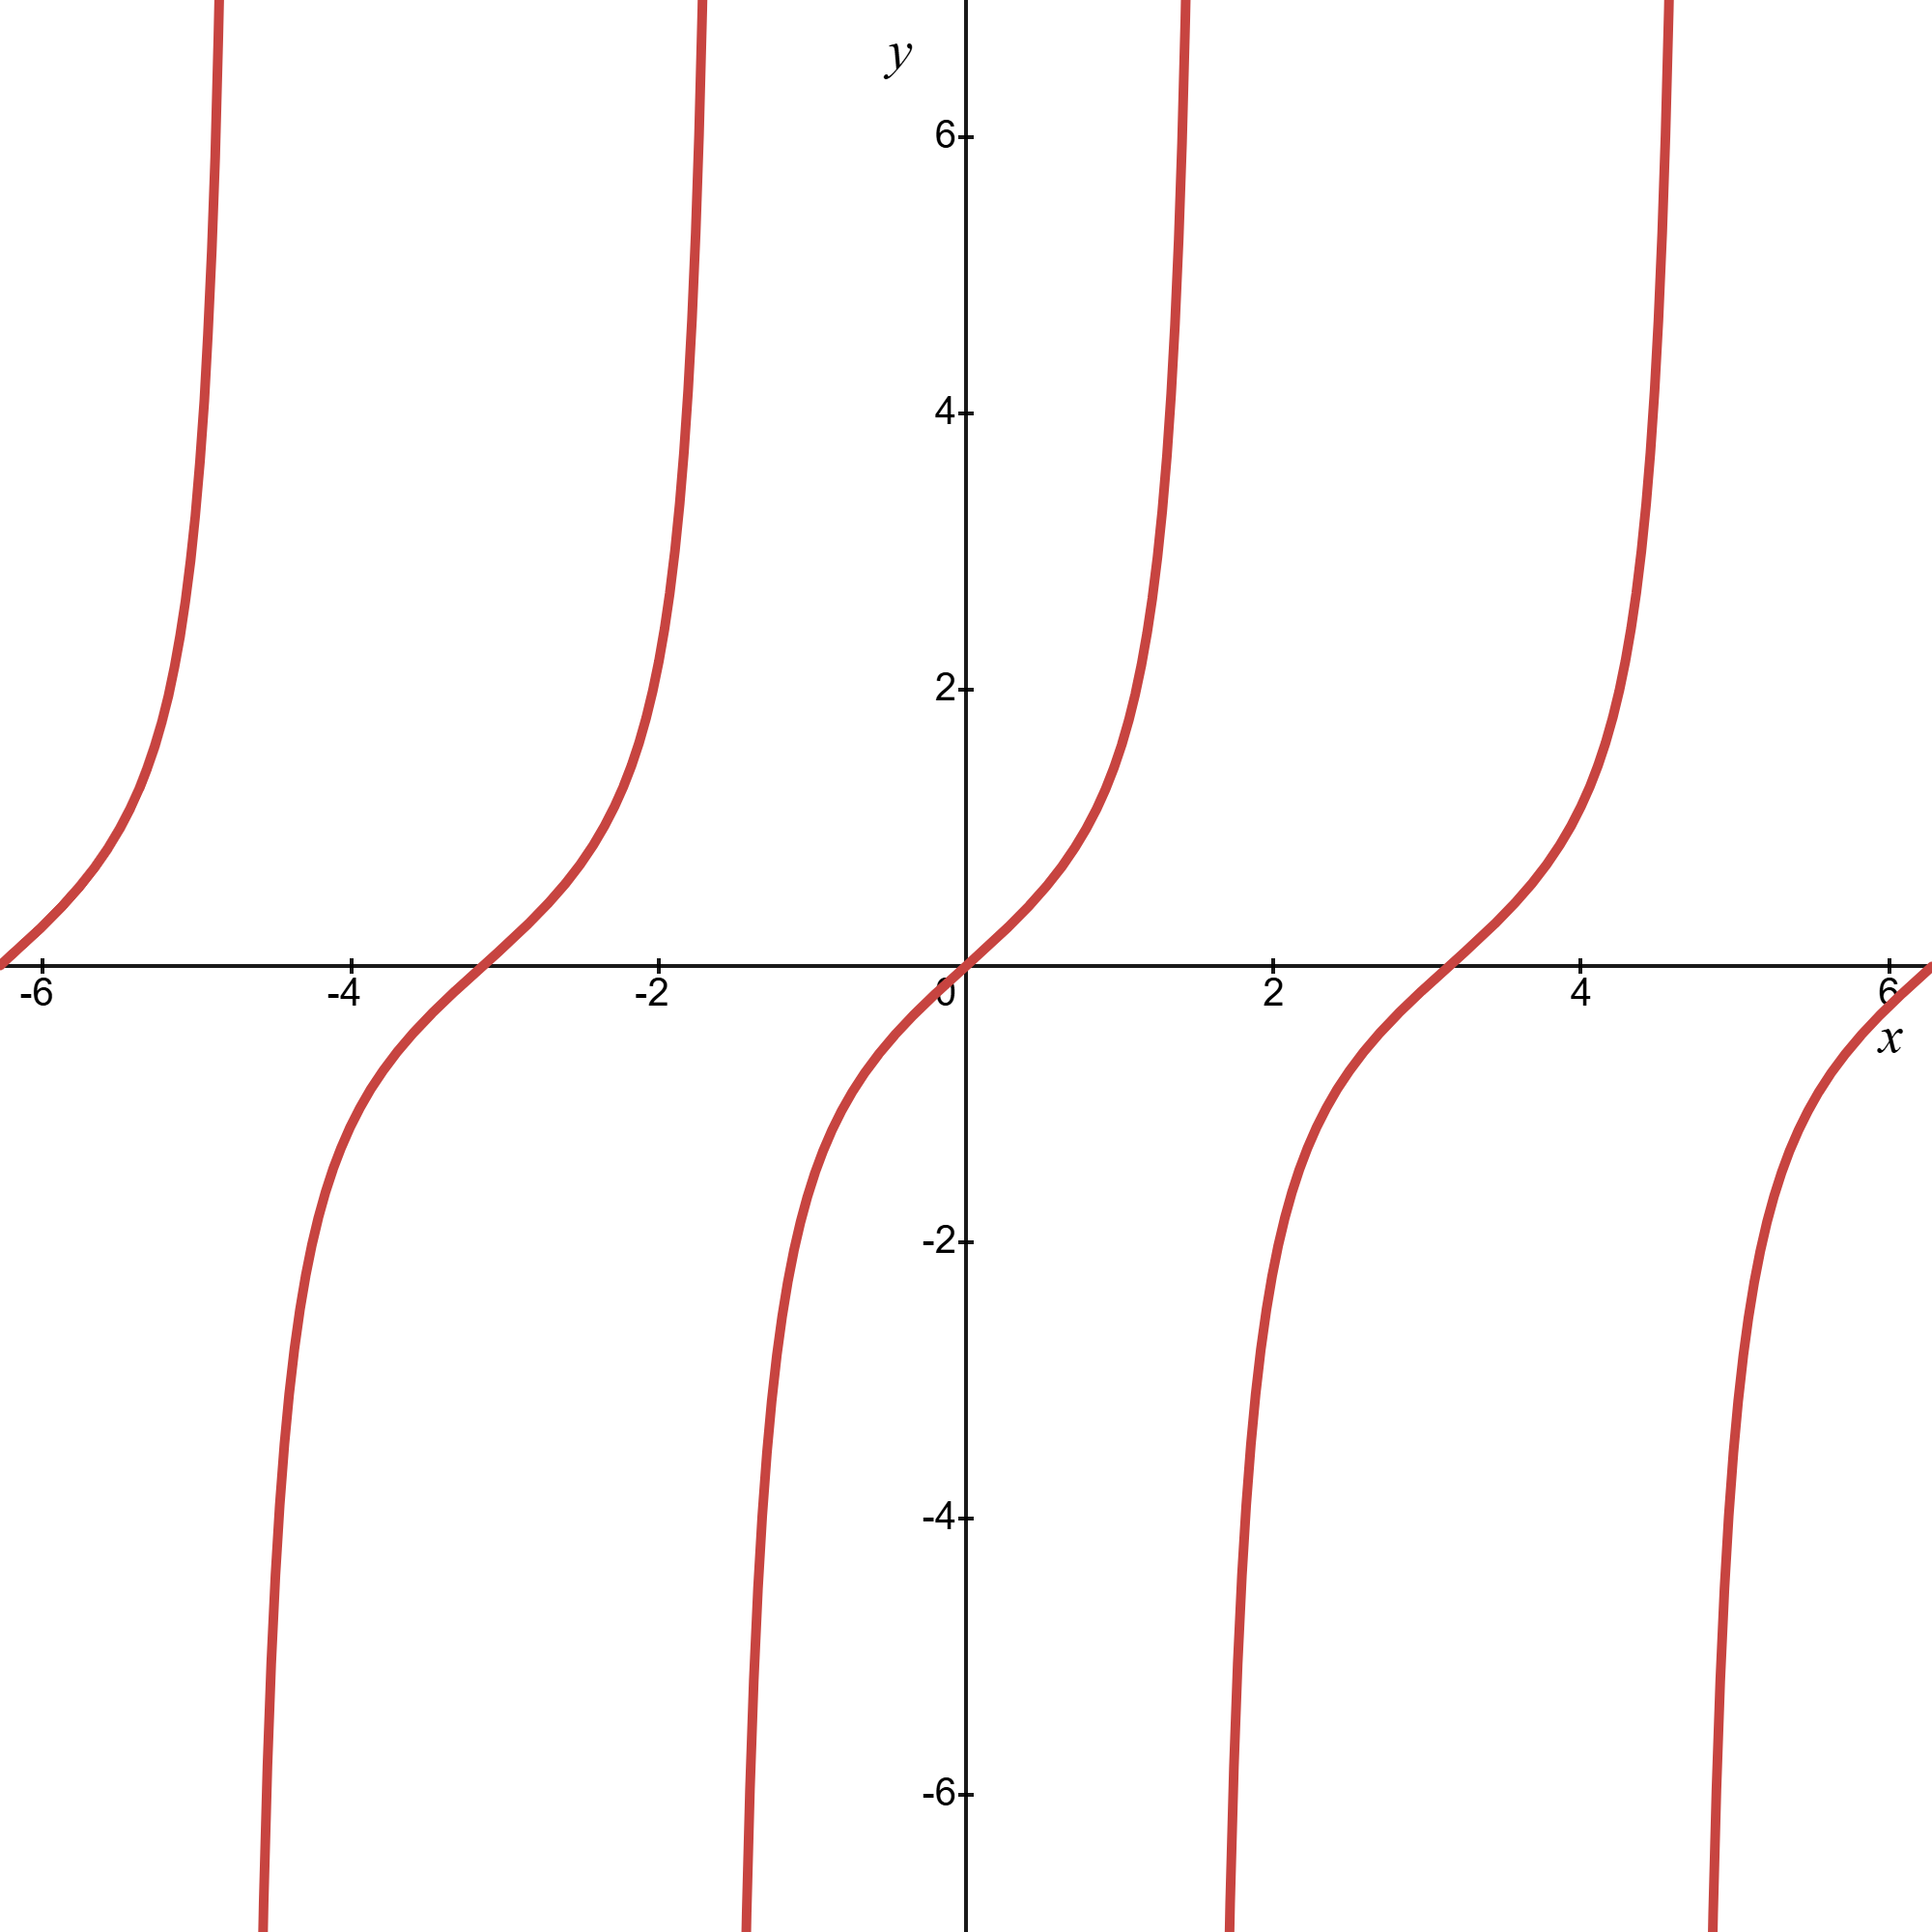
\includegraphics[width=0.45\textwidth, alt ={Graph of a tan(x).}]{figures/tan_graph}
  %}{A plot of the tan function. }
    \caption{A plot of the trig function $\tan(x)$, unlike $\sin$ and $\cos$ above, $\tan$ cannot be drawn without taking your pen off the page.  }
\label{fig: tan function}
\end{figure}

The trig functions are clearly not one-to-one, since they are periodic, in fact even restricted to $x\in[0,2\uppi)$ there are repeated values. However, just like with the square root, it is convenient to introduce inverse functions, where we need to be careful which quadrant our angle is in to get a single value out. These inverse functions are often denoted
\begin{align*}
\sin^{-1}(x)&=\arcsin(x),\\
\cos^{-1}(x)&=\arccos(x),\\
\tan^{-1}(x)&=\arctan(x).
\end{align*}

Your calculator will have a button for each trig function, and a way to select the inverse functions, typically calculators return answers in the following ranges:
\begin{equation*}
0\leq \arccos(x)\leq \uppi,\qquad -\frac{\uppi}{2}\leq \arcsin(x)\leq \frac{\uppi}{2}, \qquad -\frac{\uppi}{2}< \arctan(x)< \frac{\uppi}{2}.
\end{equation*}

The inverse trig functions are useful if we need to solve equations involving trig functions.\\

\begin{ex}
Find the solutions to $4\cos(t)=3$ for $t\in[-8,10]$. \\

The first step is to divide both sides by $4$ to give us
\begin{equation*}
\cos(t)=\frac{4}{3},
\end{equation*}
now we can use
\begin{equation*}
t=\arccos\left(\frac{3}{4}\right)=0.7227.
\end{equation*}

Not that this is just one of an infinite\footnote{``Why infinitely many?'' you ask. This is because $\cos(x)$ is $2\uppi$ periodic so if $t$ is a solution in the range $[0,2\uppi)$ then $t+2\uppi n$ is another solution for $n\in \Z$. } number of solutions to the above equation. in the range from $0$ to $2\uppi$ there are two solutions, $t=0.7227$ and $t=2\uppi-0.7227=5.5605$. We now add $2\uppi n$ to both of our values, testing values of $n$ so that the result stays within the interval :
%\begin{align*}
%&n=-2 \quad t=0.7227-4\uppi = \sout{-11.8437} \quad \text{and} \quad 5.5605-4\uppi=-7.0059\\
%&n=-1 \quad t=0.7227-2\uppi = -5.5605\quad \text{and} \quad 5.5605-2\uppi=-0.7227\\
%&n=0 \quad t=0.7227\quad \text{and} \quad 5.5605\\
%&n=1 \quad t=0.7227+2\uppi = 7.0059 \quad \text{and} \quad 5.5605+2pi=\sout{11.8437}
%\end{align*}

\begin{itemize}
%\setlength{\itemsep}{-5pt}
    \item $n=-2$  then $ t=0.7227-4\uppi =\cancel{-11.8437}$ and $t=5.5605-4\uppi=-7.0059$,
    \item $n=-1$ then $ t=0.7227-2\uppi = -5.5605$ and $t=5.5605-2\uppi=-0.7227$,
    \item $n=0$ then $t=0.7227$ and $t=5.5605$,
    \item $n=1$  then $t=0.7227+2\uppi = 7.0059$ and $ t=5.5605+2\uppi=\cancel{11.8437}$.
\end{itemize}
Thus there are six solutions in the interval $[-8,10]$,
\begin{equation*}
t=-7.0059, -5.5605, -0.7227, 0.7227, 5.5605, 7.0059.
\end{equation*}
Not that the solutions come in positive and negative pairs.
\end{ex}

You will have the opportunity to practice more problems like this either by going through the week one tutorial sheet or by looking at Section 1.5 in \citep{calcI}.\\

The trig functions satisfy some nice relationships that you should try to learn, and which we quote here without any proof. Some of these are fairly easy to prove and are left as an exercise, while others are harder and can be looked up if you are curious.\\

The first one is that 
\begin{equation*}
\tan(x)=\frac{\sin(x)}{\cos(x)}.
\end{equation*}

\paragraph{Squares:} The squares of trig functions have the nice property that
\begin{equation*}
\sin^{2}x+\cos^{2}x =1,
\end{equation*}
which is a consequence of Pythagoras' theorem.

\paragraph{Multiple angles:} There are some very useful identities when we consider trig functions for the sum and difference of an angle:
\begin{align*}
\sin\left(x\pm y\right)&=\sin x \cos y \pm \cos x \sin y,\\
\cos\left(x\pm y\right)&=\cos x \cos y \mp \sin x \sin y.
\end{align*}
For the special case of $x=y$ this leads to 
\begin{align*}
\sin 2x &= 2\sin x \cos x,\\
\cos 2x &=\cos^{2}x-\sin^{2}x = 2\cos^{2}x -1 =1-2\sin^{2}x.
\end{align*}

You should try to become familiar with these identities, at least for this module, as they will be useful wherever trig functions appear.\\

\paragraph{Further trig functions:} There are three more trig functions that you should be aware of. Again, these are not independent trig functions but are one over the familiar trig functions. These are:
\begin{align*}
\sec x &=\frac{1}{\cos x},\\
\csc x &=\frac{1}{\sin x},\\
\cot x &=\frac{1}{\tan x}.
\end{align*}
Plots of these three functions are shown in \cref{fig: sec function}.

\begin{figure}[ht]
    \centering
  %  \pdftooltip{
  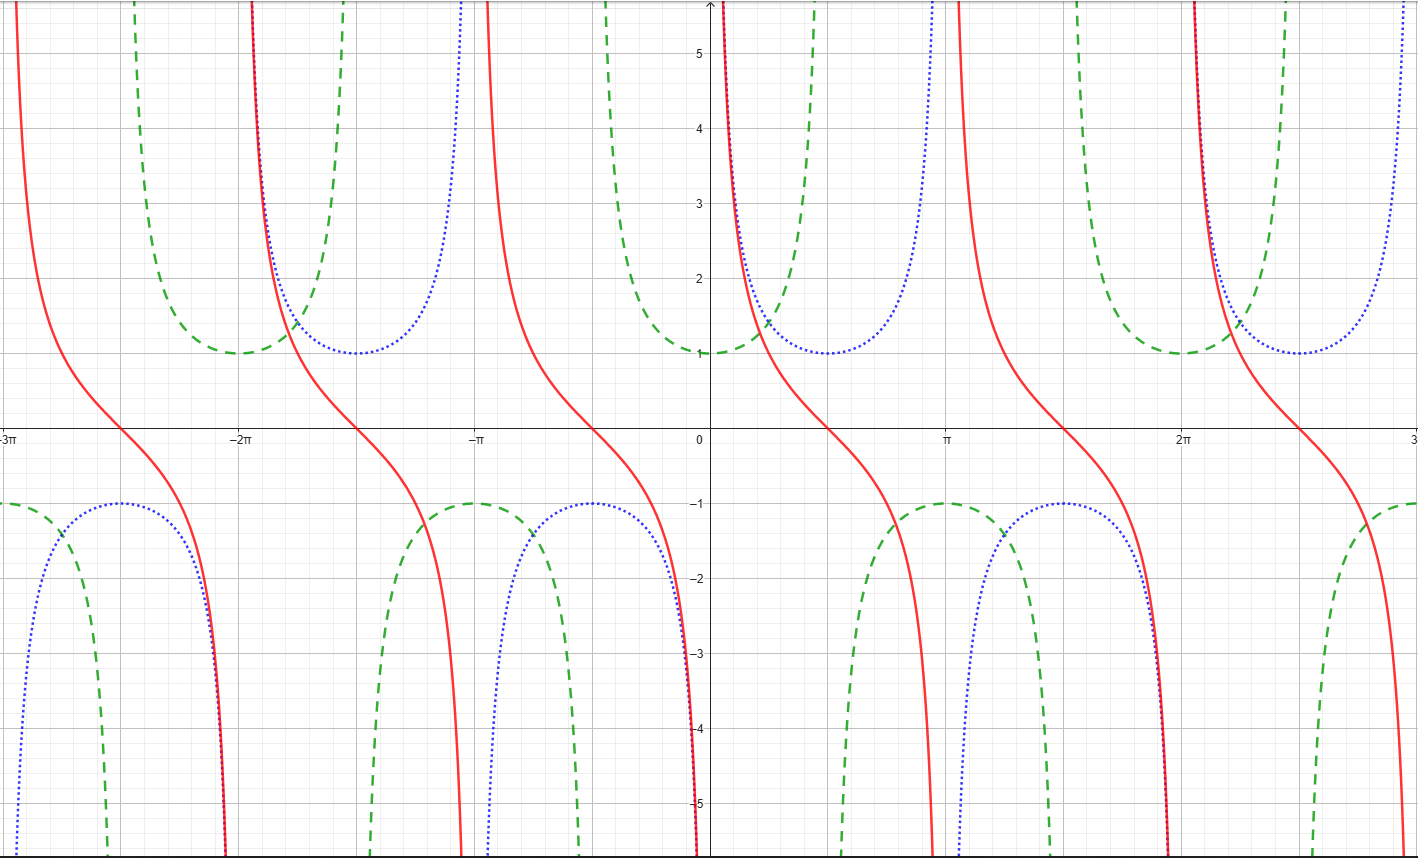
\includegraphics[width=0.8\textwidth, alt ={Graphs of sec(x), csc(x), and cot(x).}]{figures/sec-cot-csc-fig}
  %}{A plot of the other trig function. }
    \caption{A plot of the trig functions produced using GeoGebra: $\sec(x)$ the green dashed line, $\csc(x)$ the blue dotted line, and $\cot(x)$ the solid red line. It is not possible to draw any of these functions without taking the pen off the page, we will see later that this is because these functions have vertical asymptotes where the functions head off to infinity.  }
\label{fig: sec function}
\end{figure}

\section{Logarithms and Exponentials}
\label{sec: log and exp}

Another pair of very useful functions which we need to be familiar with are the logarithm and the exponential function. \\

In your previous maths courses you may have come across the fact that we call powers exponents, e.g. in an expression $f(x)=x^{b}$ then $b$ is called the exponent,, or the index. An exponential function is then a function like
\begin{equation*}
f(x)=b^{x},
\end{equation*}
where a constant\footnote{here $b>0$ and $b\neq 1$.} $b$ is raised to the power of the variable $x$. In this case the number $b$ is called the \textbf{\gls{base}} of the exponential function.\\

The exponential function with base $2$ is shown in \cref{fig: exp and log 1}.  It turns out that by appropriate scaling of $x$ different bases are related\footnote{To get an idea of this consider that $2^{x}=4^{x/2}$ so we can always transform from base $2$ into base $4$. In general we need to use the logarithm function that we will meet shortly.} so we only need one standard basis. \\

When working with binary the basis $b=2$ is chosen, while in scientific notation $b=10$ is chosen.  Nowadays the basis in general use is denoted $e$ or $\exp$ with $\exp(x)$ called the \textbf{exponential function}. \\

\begin{mdiv}
\textbf{Warning}! When talking to mathematicians there is a difference between $e$ and $\exp$, the first one is a number, close to $2.71828\dots$, while $\exp$ is a function. Often we will use $e^{x}$ and $\exp(x)$ interchangeably, but occasionally it is important to know the difference.  The main difference is that $\exp(x)$ is a one-to-one function, in particular  when $x=1/2$ we have that $\exp(1/2)\simeq 1.65$ while when taking $\sqrt{e}=e^{1/2}$ we need to pick either the positive or negative square root.  Most likely you can just forget this distinction and work with $e^{x}$ and $\exp(x)$ as if they were the same thing. However, it is worth seeing the distinction at least once.
\end{mdiv}

\begin{figure}[ht]
    \centering
\ThisAltText{Graph of exponential and logarithm functions with base 2.}
 %   \pdftooltip{
    \begin{tikzpicture}[line width=1pt,line cap=round,line join=round, smooth,variable=\x]
     \draw[->] (-3.8,0) -- (5,0) node[above] {$x$};
  \draw[->] (0,-4) -- (0,5)node[above]{$y$};
 \draw[color=CDnavy, domain=-3.8:2.3]   plot[samples=300] (\x,{2^(\x)}) node[right] {$2^{x}$};
  \draw[color=CDgreen, domain=0.06:4]   plot[samples=300] (\x,{log2(\x )}) node[anchor = north west] {$\log_2(x)$};
  \draw[ dashed, color = gray, domain = -2.5:4.5] plot (\x,\x)node[right]{$y=x$};
    \end{tikzpicture}
%    }{plots of an exponential and logarithm }
    \caption{Plots of the exponential and logarithm functions, $y=2^{x}$ and $y=\log_{2}(x)$.}
        \label{fig: exp and log 1}
\end{figure}

The reason for picking $e$ as the basis is that simplifies some of the algebra associated with exponential functions, it also has the advantage that the tangent to the curve has gradient $1$ at $x=0$. This last part boils down to 
\begin{equation}
e\simeq \left(1+h\right)^{\frac{1}{h}} 
\label{eq: exp approximation}
\end{equation}
for $h$ close to zero. 

\begin{figure}[ht]
    \centering
\ThisAltText{Graph of exponential and logarithm functions with base e.}
%    \pdftooltip{
    \begin{tikzpicture}[line width=1pt,line cap=round,line join=round, smooth,variable=\x, ]
     \draw[->] (-3.6,0) -- (5,0) node[above] {$x$};
  \draw[->] (0,-4) -- (0,5)node[above]{$y$};
 \draw[color=CDnavy, domain=-3.8:1.6]   plot[samples=300] (\x,{exp(\x)}) node[right] {$\exp(x)$};
  \draw[color=CDgreen, domain=0.03:4]   plot[samples=300] (\x,{ln(\x )}) node[anchor = north west] {$\ln(x)$};
  \draw[ dashed, color = gray, domain = -2.5:4.5] plot (\x,\x)node[right]{$y=x$};
    \end{tikzpicture}
%    }{plots of exp and ln }
    \caption{Plots of the exponential and logarithm functions, $y=\exp(x)$ and $y=\ln(x)$.}
        \label{fig: exp and log 2}
\end{figure}

Closely related to $\exp$ is its inverse function, called the \textbf{logarithm} function. You will see it written as either $\log(x)$ or $\ln(x)$, or rarely as $\log_{e}(x)$ where the base is made explicit. \\

As this is an inverse function it is defined as the solution to the equation $e^{y}=x$. For example $e^{y}=4$ is solved by $y=\ln(4)$.\\

The graphs of both $\exp(x)$ and $\ln(x)$ are shown in \cref{fig: exp and log 2}. Note that we are, currently, not defining $\ln$ when $x$ is negative \footnote{If you study more mathematics you will discover that we can make sense of $\ln(x)$ when $x$ is negative. However, it is no longer real and we need to understand complex numbers to make sense of it.}.  You may have guessed that we could take a logarithm in a different basis since it is defined so that
\begin{equation*}
\ln(\exp(x))=x=\exp(\ln(x)).
\end{equation*}

This is why there are several slightly different ways of writing the logarithm. If you learnt about it in school you probably used $\log(x)$ to mean log with base $10$. In this module if we work with a basis other than $e$ we will make this explicit by writing $\log_{b}(x)$ to mean log with base $b$.\\

To be clear $\log_{b}(x)$ is the function defined such that
\begin{equation*}
\log_{b}(b^{x})=x=b^{\log_{b}(x)}.
\end{equation*}

A nice property of exponentials and logarithms is that they map addition to multiplication. What this means is that
\begin{align*}
\exp(a)\exp(b)&=\exp(a+b),\\
\ln(ab)&=\ln(a)+\ln(b),\\
\ln\left(\frac{a}{b}\right)&=\ln(a)-\ln(b).
\end{align*}

Some of the other properties of these functions are that:
\begin{align*}
\exp(-x)&=\frac{1}{\exp(x)},\\
\exp(x)&>0,\\
\exp(x)&\to \infty \quad \text{as } x\to \infty,\\
\exp(x)&\to 0 \quad \text{as } x\to -\infty,\\
\ln(x) &\to \infty \quad \text{as } x\to \infty,\\
\ln(x)&\to -\infty \quad \text{as } x\to 0^{+}.
\end{align*}
We will return to discussing limits shortly, but here the statement $\exp(x)\to \infty$ as $x\to \infty$ means that the function $\exp(x)$ becomes infinitely large as $x$ becomes infinitely large. The terminology for this is that $\exp(x)$ \textbf{diverges} as $x$ tends to infinity.\\

The final, useful, identity about logarithms is how to change the basis. The change of basis formula is
\begin{equation}
\log_{b}(x)=\frac{\log_{a}(x)}{\log_{a}(b)}.
\label{eq:log change of base}
\end{equation}

As with trig functions in \cref{sec: trig func}, $\ln$ and $\exp$ are useful when solving equations. There are lots of examples in \citep{calcI} but we will go through a couple of examples here, there will be more on the tutorial sheets.

\begin{ex}
Consider the equation
\begin{equation*}
x e^{-x} -x =0.
\end{equation*}
The first step in solving this is to factor out the $x$ common to both terms. Note that we \textbf{cannot} divide by $x$ as at this stage we do not know if it will be zero. This gives us
\begin{align*}
x e^{-x} -x &=0\\
x\left(e^{-x}-1\right)&=0,
\end{align*}
so we get two possibilities\footnote{Sometimes we will get more than two possibilities, remember with trig functions their periodicity meant that we had infinitely many solutions.}: either $x=0$ or $e^{-x}-1=0$. If we had divided by $x$ we would have missed that $x=0$ is a solution, and would not have completely solved the problem. Consider the second case,
\begin{align*}
e^{-x}&=1\\
-x&=\ln(1)=0
\end{align*}
so this other case also reduces to $x=0$ and we only have one solution in this case.
\end{ex}

\begin{ex}
\label{ex: log equation}
Consider the equation
\begin{equation*}
\frac{1}{2}\ln\left(x^{2}\right)-\ln\left(x-1\right)=4.
\end{equation*}
If we make use of the log rules we have that $\ln(x^{2})/2=\ln(\sqrt{x^{2}})=\ln x$, where we take the positive square root as currently we do not know how to make sense of logarithms with negative arguments. The equation thus becomes
\begin{align*}
4&=\frac{1}{2}\ln\left(x^{2}\right)-\ln\left(x-1\right)\\
&=\ln\left(x\right)-\ln\left(x-1\right)\\
&=\ln\left(\frac{x}{x-1}\right).
\end{align*}
Now we can exponentiate both sides and rearrange to solve for $x$:
\begin{align*}
\frac{x}{x-1}&=e^{4}\\
x&=e^{4}\left(x-1\right)\\
x&=-e^{4}+xe^{4}\\
x\left(1-e^{4}\right)&=-e^{4}\\
x&=-\frac{e^{4}}{1-e^{4}}=1.01866.
\end{align*}

When we get an answer like this we need to check that it does not give a negative argument in any of the original logarithms, here we are fine since both $x^{2}$ and $x-1$ are positive.

\end{ex}

It may seem like example~\ref{ex: log equation} took quite a bit of working out, but with practice you will get faster at solving problems like this. In the lectures you will frequently hear me paraphrasing George P\'{o}lya and saying that Mathematics is not a spectator sport. This means that while reading these notes and attending the lectures can help you in your learning there is no substitute for actually rolling your sleeves up and solving problems. Remember that most modules \textit{expect} you to be putting in around three hours of self study for every hour of contact time.

\section{Hyperbolic functions}
\label{sec: hyperbolic functions}
The next class of functions that it is useful to know about are the \textbf{hyperbolic} trig functions. As shown in \cref{fig: hyperbolic functions}, the hyperbolic trig functions are the analogue of the standard trig functions of \cref{sec: trig func} but adapted to the geometry of the hyperbola, $x^{2}-y^{2}=1$ rather than the circle $x^{2}+y^{2}=1$. For the standard trig functions, their argument was an angle related to how far round the unit circle we had gone. In the hyperbolic case the \textit{angle} is now twice the shaded area shown in \cref{sec: trig func}. \\

\begin{figure}[ht]
    \centering
  %  \pdftooltip{
  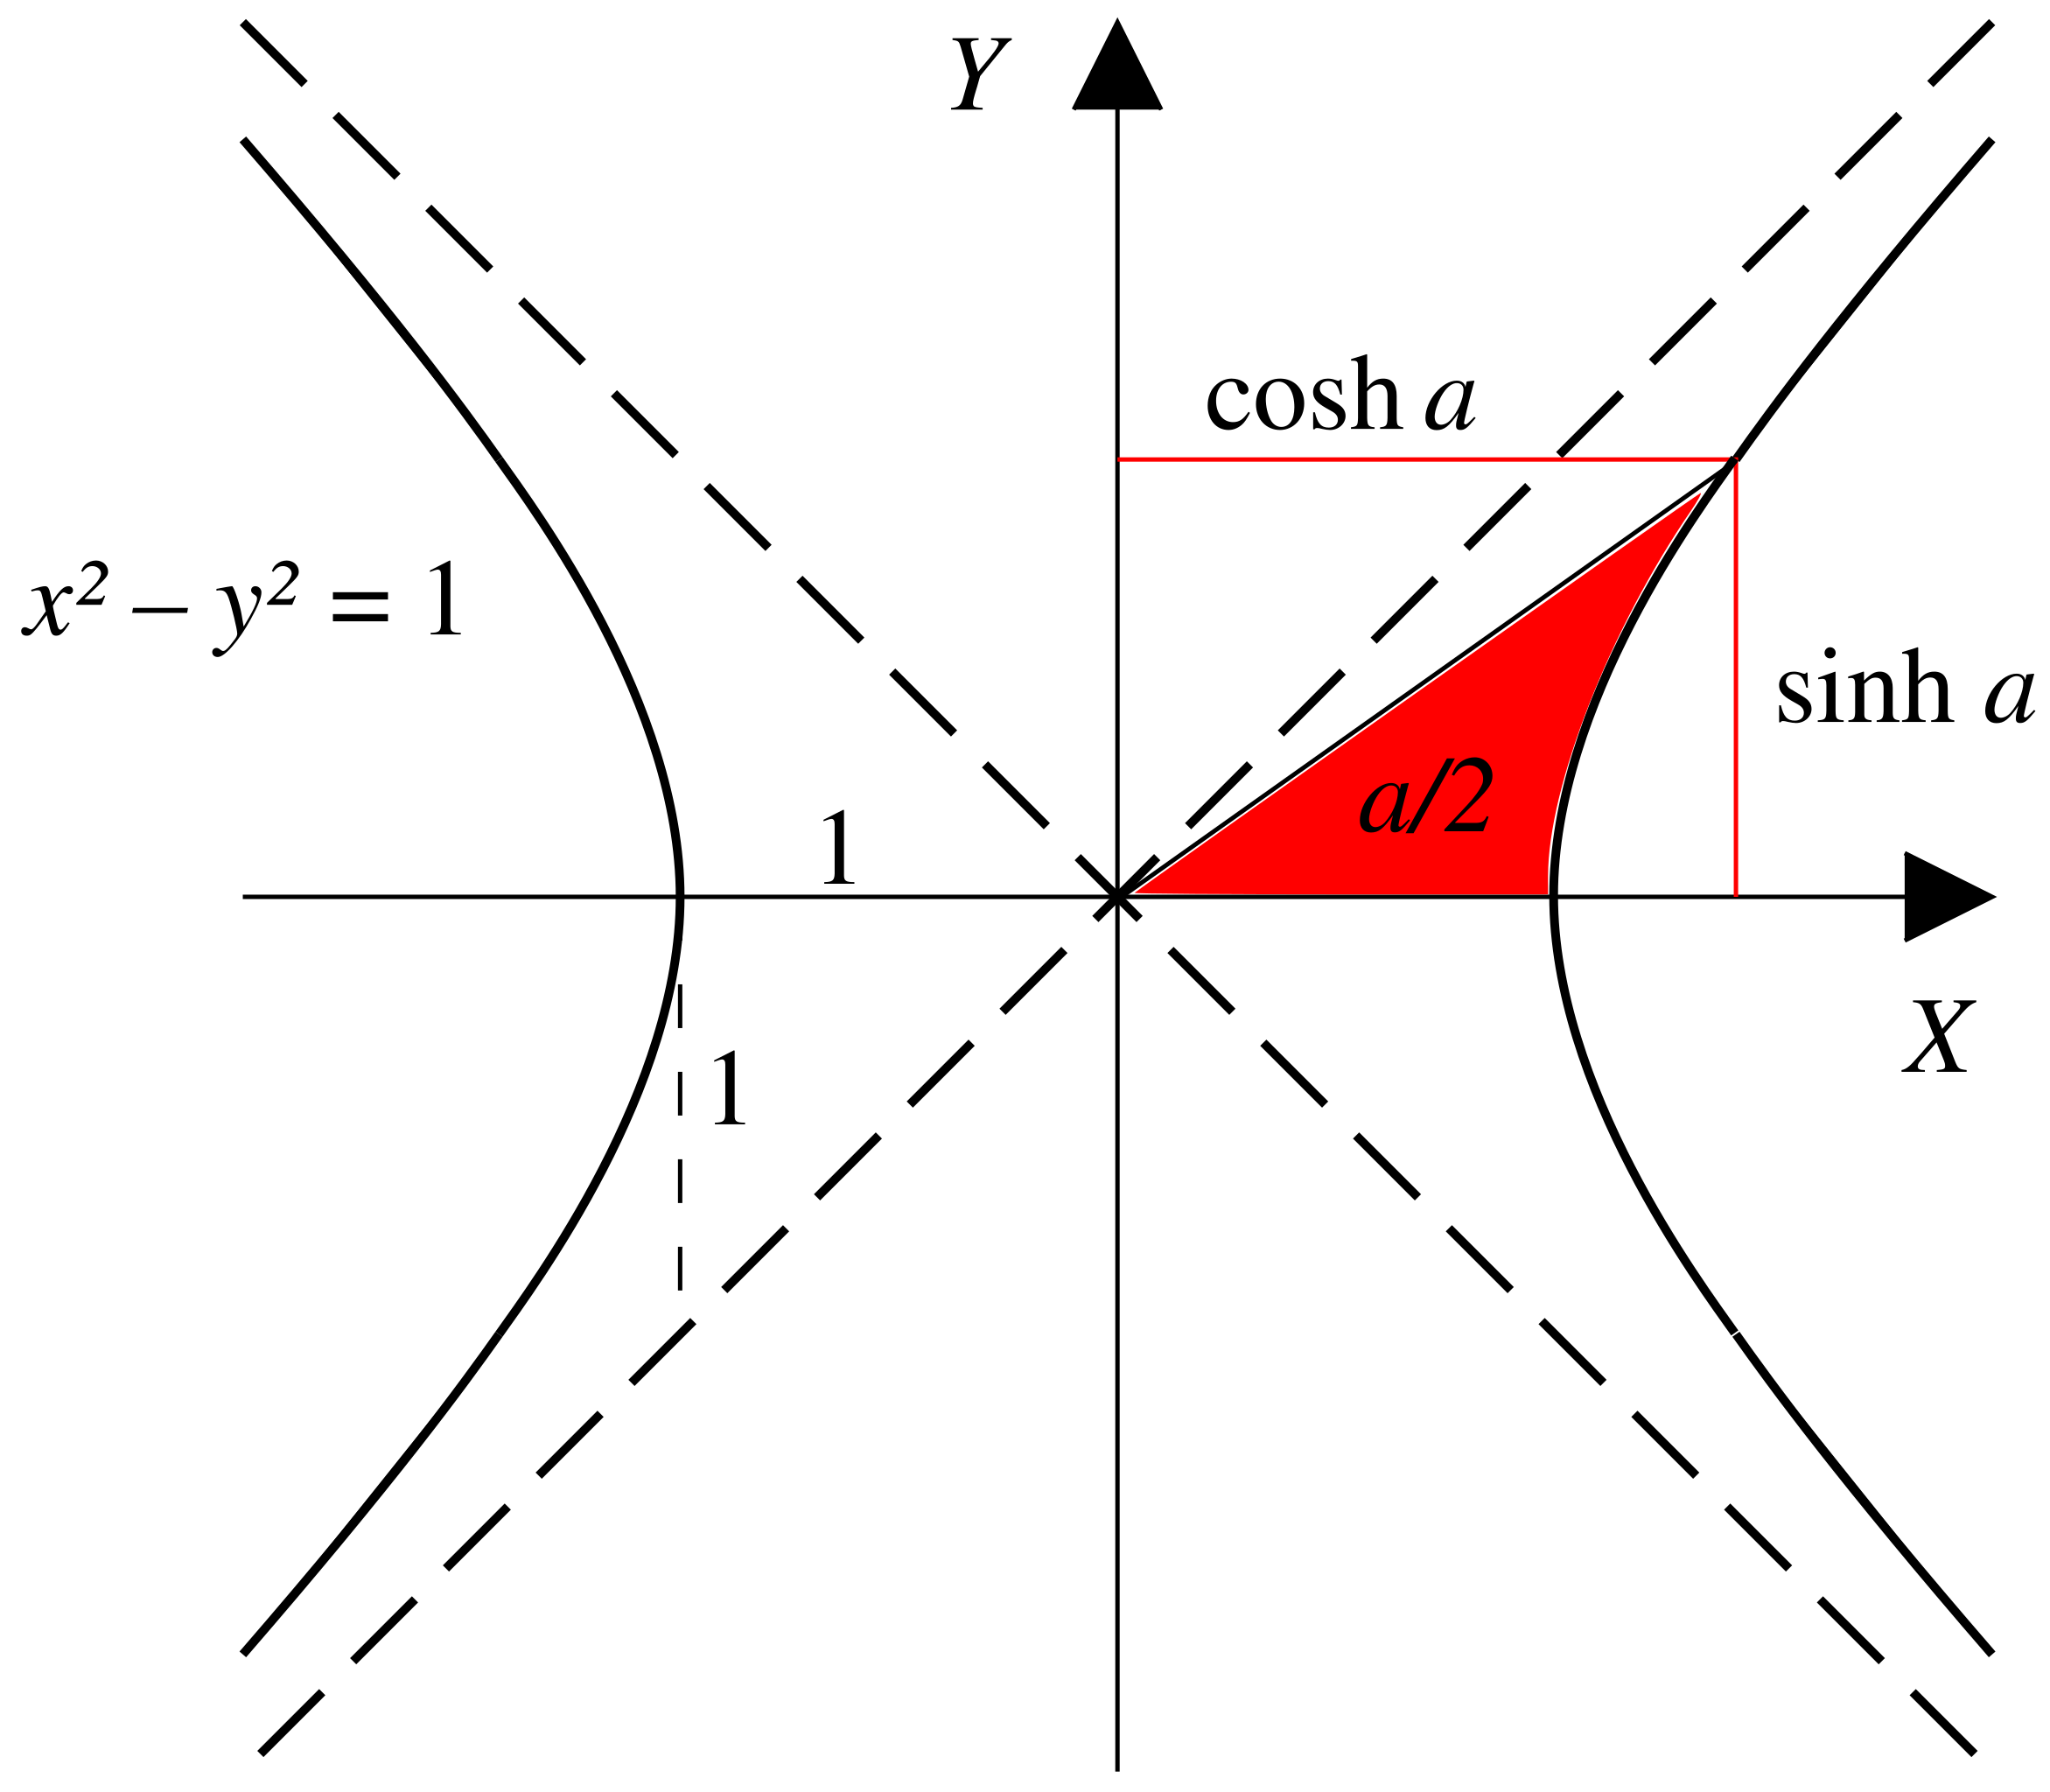
\includegraphics[width=0.4\textwidth, alt ={Hyperbolic trig functions are related to the geometry of hyperbolas rather than circles.}]{figures/Hyperbolic_functions}
  %}{A plot of the tan function. }
    \caption{Hyperbolic trig functions are defined in terms of  the area enclosed by a radial ray and the hyperbola $x^{2}-y^{2}=1$.  The convention is to assume that $a$ is negative for points below the $x$-axis. The image is from \href{https://commons.wikimedia.org/wiki/File:Hyperbolic_functions-2.svg}{Wikimedia commons}. }
\label{fig: hyperbolic functions}
\end{figure}


There is a hyperbolic equivalent of all of the standard trig functions, and the notation is very similar just with an added $h$ at the end:
\begin{itemize}
%\setlength{\itemsep}{-5pt}
    \item \textbf{hyperbolic sine}  $\sinh$,
    \item \textbf{hyperbolic cosine} $\cosh$,
   \item \textbf{hyperbolic tangent} $\tanh$,
   \item \textbf{inverse hyperbolic sine} $\arcsinh$,
   \item \textbf{inverse hyperbolic cosine} $\arccosh$,
   \item \textbf{inverse hyperbolic tangent} $\arctan$.
\end{itemize}
There are also hyperbolic versions of the other trig functions but we will not be as concerned with them here.\\

As in the regular trig case the hyperbolic tangent is defined in terms of the other two functions as
\begin{equation}
\tanh(x)=\frac{\sinh(x)}{\cosh(x)}.
\label{eq: hyperbolic tangent}
\end{equation}

The hyperbolic trig functions are actually defined in terms of the odd and even parts of the exponential function\footnote{If you have come across complex numbers then you may know that this is only true for real $x$, if the argument is imaginary then relationships like this hold between the exponential function and the standard trig functions. We may see this in the advanced topics section of the module if there is enough time.} as follows:
\begin{align}
\sinh(x)&=\frac{e^{x}-e^{-x}}{2}, \label{eq: sinh exp}\\
\cosh(x)&=\frac{e^{x}+e^{-x}}{2}. \label{eq: cosh exp}
\end{align}
They have the following useful properties:
\begin{align*}
\sinh(-x)&=-\sinh(x),\\
\cosh(-x)&=\cosh(x),\\
\cosh^{2}(x)-\sinh^{2}(x)&=1,\\
1-\tanh^{2}(x)&=\sech^{2}(x).
\end{align*}
These are very similar to the identities satisfied by the ordinary trig functions. However, the sign in front of $\sinh(x)$ and $\tanh(x)$ is negative while that in front of $\sin(x)$ and $\tan(x)$ in the equivalent formulae was positive. The rule of thumb when converting from identities for trig functions to identities for hyperbolic trig functions is to send $\cos^{2}(x)\to \cosh^{2}(x)$ and $\sin^{2}(x)\to -\sinh^{2}(x)$.  There are also analogues of the addition of angle identity formulas that you can try to derive if you are interested.\\


\begin{ex}
Consider the hyperbolic equation $\cosh(x)-5\sinh(x)-5=0$ from chapter 3.7 in \citep{riley_mathematical_2006}. The easiest way to solve this is to use the definitions of the hyperbolic functions in terms of the exponential function. This transforms the equation into
\begin{equation*}
\frac{1}{2}\left(e^{x}+e^{-x}\right)-\frac{5}{2}\left(e^{x}-e^{-x}\right)-5=0,
\end{equation*}
which we rearrange to give
\begin{equation*}
0=e^{x}\left(\frac{1}{2}-\frac{5}{2}\right)+e^{-x}\left(\frac{1}{2}+\frac{5}{2}\right)-5=-2e^{x}+3e^{-x}-5.
\end{equation*}
Then multiply through by $-e^{x}$, which is allowed since this is never zero, to get
\begin{equation*}
2e^{2x}+5e^{x}-3=0.
\end{equation*}
Now we could either let $y=e^{x}$ and use the quadratic formula to solve for $y$ or we can factorise this to get
\begin{equation*}
\left(2e^{x}-1\right)\left(e^{x}+3\right)=0,
\end{equation*}
so there are two solutions: $e^{x}=1/2$ or $x=-\ln(2)$, and $e^{x}=-3$ or $x=\ln(-3)$. Remember we have not discussed how to make sense of the logarithm of a negative number so for us there is only one real solution, $x=-\ln(2)$.
\end{ex}

Since the hyperbolic trig functions are related to the exponential function you can probably guess that their inverses are related to the logarithm. It is worth thinking about how to show this relationship. I will show you how to do this for $\sinh(x)$ and $\tanh(x)$ but leave deriving the identify for $\cosh(x)$ as an exercise for the interested reader.

\begin{ex}
Consider $y=\arcsinh(x)$, we can invert this to give $x=\sinh(y)$. Next if we make use of \cref{eq: sinh exp,eq: cosh exp} we have that
\begin{align*}
e^{y}	&=\cosh(y)+\sinh(y)\\
	&=\sqrt{1+\sinh^{2}(y)}+\sinh(y)\\
	&=\sqrt{1+x^{2}}+x.
\end{align*}
Taking $\ln$ of both sides then gives that
\begin{equation}
\arcsinh(x)=y=\ln\left(\sqrt{1+x^{2}}+x\right).
\label{eq: arcsinh log}
\end{equation}
\end{ex} 

If you do a similar calculation for $y=\arccosh(x)$ you will find that
\begin{equation}
\arccosh(x)=\ln\left(x\pm \sqrt{x^{2}-1}\right).
\label{eq: arccosh log}
\end{equation} 

You should think about why there is a $\pm$ in this formula but there was not one in \cref{eq: arcsinh log}.

\begin{ex}
Consider $y=\arctanh(x)$, which inverts to $x=\tanh(y)$. Using the definition of $\tanh(y)$ as being $\sinh(y)/\cosh(y)$ and \cref{eq: sinh exp,eq: cosh exp}  we have that
\begin{equation*}
x=\frac{e^{y}-e^{-y}}{e^{y}+e^{-y}}
\end{equation*}
which is equivalent to 
\begin{equation*}
\left(x+1\right)e^{-y}=\left(1-x\right)e^{y}.
\end{equation*}
which can be further rearranged to give
\begin{align*}
e^{2y}&=\frac{1+x}{1-x},\\
\Rightarrow e^{y}&=\sqrt{\frac{1+x}{1-x}},\\
y&=\ln\left(\sqrt{\frac{1+x}{1-x}}\right).
\end{align*}
This gives that 
\begin{equation}
\arctanh(x)=\frac{1}{2}\ln\left(\frac{1+x}{1-x}\right).
\label{eq: arctanh log}
\end{equation} 

\end{ex}

You may be asking why we have spend the time deriving these identities for the hyperbolic functions, and why we discussed their relationship with the exponential function. This is because when we start to differentiate or integrate hyperbolic functions it is often more straightforward to use the expressions involving exponentials and logarithms. 


\section{Limits and asymptotics}
We have now spent quite a bit of time discussing different examples of functions and their properties, as well as how to plot them. If we consider the plot of the tangent function in \cref{fig: tan function} you may have asked at the time, what happens when the red line goes off the top of the page and reappear at the bottom? If we followed both lines we would see that they are getting closer and closer to the point $x=\uppi/2$. This idea of zooming in on a particular value $x=a$ and asking what happens to a function there is known as \textbf{taking a limit} as $x$ approaches $a$ and is denoted $\lim_{x\to a}f(x)$.\\

If the function is \textit{well behaved} at the point $a$, then the limit is just the value of the function evaluated at $a$, $f(a)$. For example
\begin{equation*}
\lim_{x\to 0}\cos(x)=1=\cos(0).
\end{equation*}
The value of the limit does not have to be finite, it can head off to infinity. A good example of this is the exponential function which just keeps getting larger as $x$ increases. We denote this by
\begin{equation*}
\lim_{x\to \infty}\exp(x)\to \infty.
\end{equation*}
Notice that since the value of the limit is infinite we do not write an equals sign but instead use $\to$ to denote that the limit \textbf{diverges}\footnote{This is just the term that mathematicians use for a function that heads off to infinity.}. There are lots of other examples of functions that diverge, and not always for large $x$. A nice example to have in mind is $y=1/x^{2}$ which diverges as $x\to 0$.\\

In the case of $\tan(x)$ we can observe that $\lim_{x\to \uppi/2}\tan(x)$ will take on different values depending on if $x$ is approaching $\uppi/2$ from above or below. This means that the limit \textbf{does not exist}. In \cref{sec: continuity} we will discuss the consequences of this for the function in more detail. If we are taking the limit from above we often say $x\to a^{+}$, while the limit from below is denoted $x\to a^{-}$. In this case
\begin{align*}
\lim_{x\to \frac{\uppi}{2}^{+}}\tan(x)&\to \infty,\\
\lim_{x\to \frac{\uppi}{2}^{-}}\tan(x)&\to -\infty,
\end{align*}
so $\tan(x)$ diverges in different directions depending on how we approach $\uppi/2$.

\begin{mdiv}
Putting our mathematician's hats on for a brief moment, we would say that limit of a function $f(x)$ as $x$ approaches $a$ is $L$ and write it as
\begin{equation*}
\lim_{x\to a}f(x)=L,
\end{equation*}
as long as we can make $f(x)$ as close to $L$ as we want for all $x$ sufficiently close to $a$ on both sides, without taking $x=a$.\\

If this was a maths module we would be even more precise and give what is called an $\upepsilon,\updelta$ definition. Fortunately for all of us this is not a maths module and we can focus on a more practical/ working  definition rather than getting bogged down in the abstract details. If you are interested to know how to do this in detail, the section ``The Definition of a Limit'' in \citep{calcI} is a good place to look.  \\

\textbf{Remember} that $x\to a$ does not mean that $x$ becomes equal to $a$, it just means that $x$ is getting close to $a$. It is also possible that $f(x)$ may never equal $L$, but also just get close to it. This is especially true when we take the limit  near a point that the function is not defined at, e.g. $x\to \uppi/2$ for $\tan(x)$.
\end{mdiv}

Curve sketching is a useful way to understand the main features of a function and can help us to know if the limit exists and if we have the same limit when approaching from different directions. 

\begin{ex}
Consider the function 
\begin{equation}
f(x)=\frac{1}{x-2},
\label{eq: reciprocal of x-2}
\end{equation}
defined for $x\neq 2$.\\

Notices that for $x\to\pm \infty$ $f(x)\to 0$, in \cref{fig: asymptotes function} we see that the plot approaches the horizontal axis \textbf{asymptotically}\footnote{The definition of asymptotically is ``approaching a given value or condition, as a variable or an expression containing a variable approaches a limit, usually infinity'' \citep{collins:asymptotically}}. We can also observe that for $a\neq 2$ $f(x)\to f(a)$ for $x\to a$.  The only point where we need to be careful is when $x$ tends to $2$ looking at \cref{fig: asymptotes function} we see that if we approach $2$ from above that $f(x)\to \infty$ while if we approach $2$ from below $f(x)\to -\infty$. \\

Note that the fact that $f(x)$ is not defined at $x=2$ has no bearing on the limiting behaviour.

\end{ex}

\begin{figure}[ht]
    \centering

  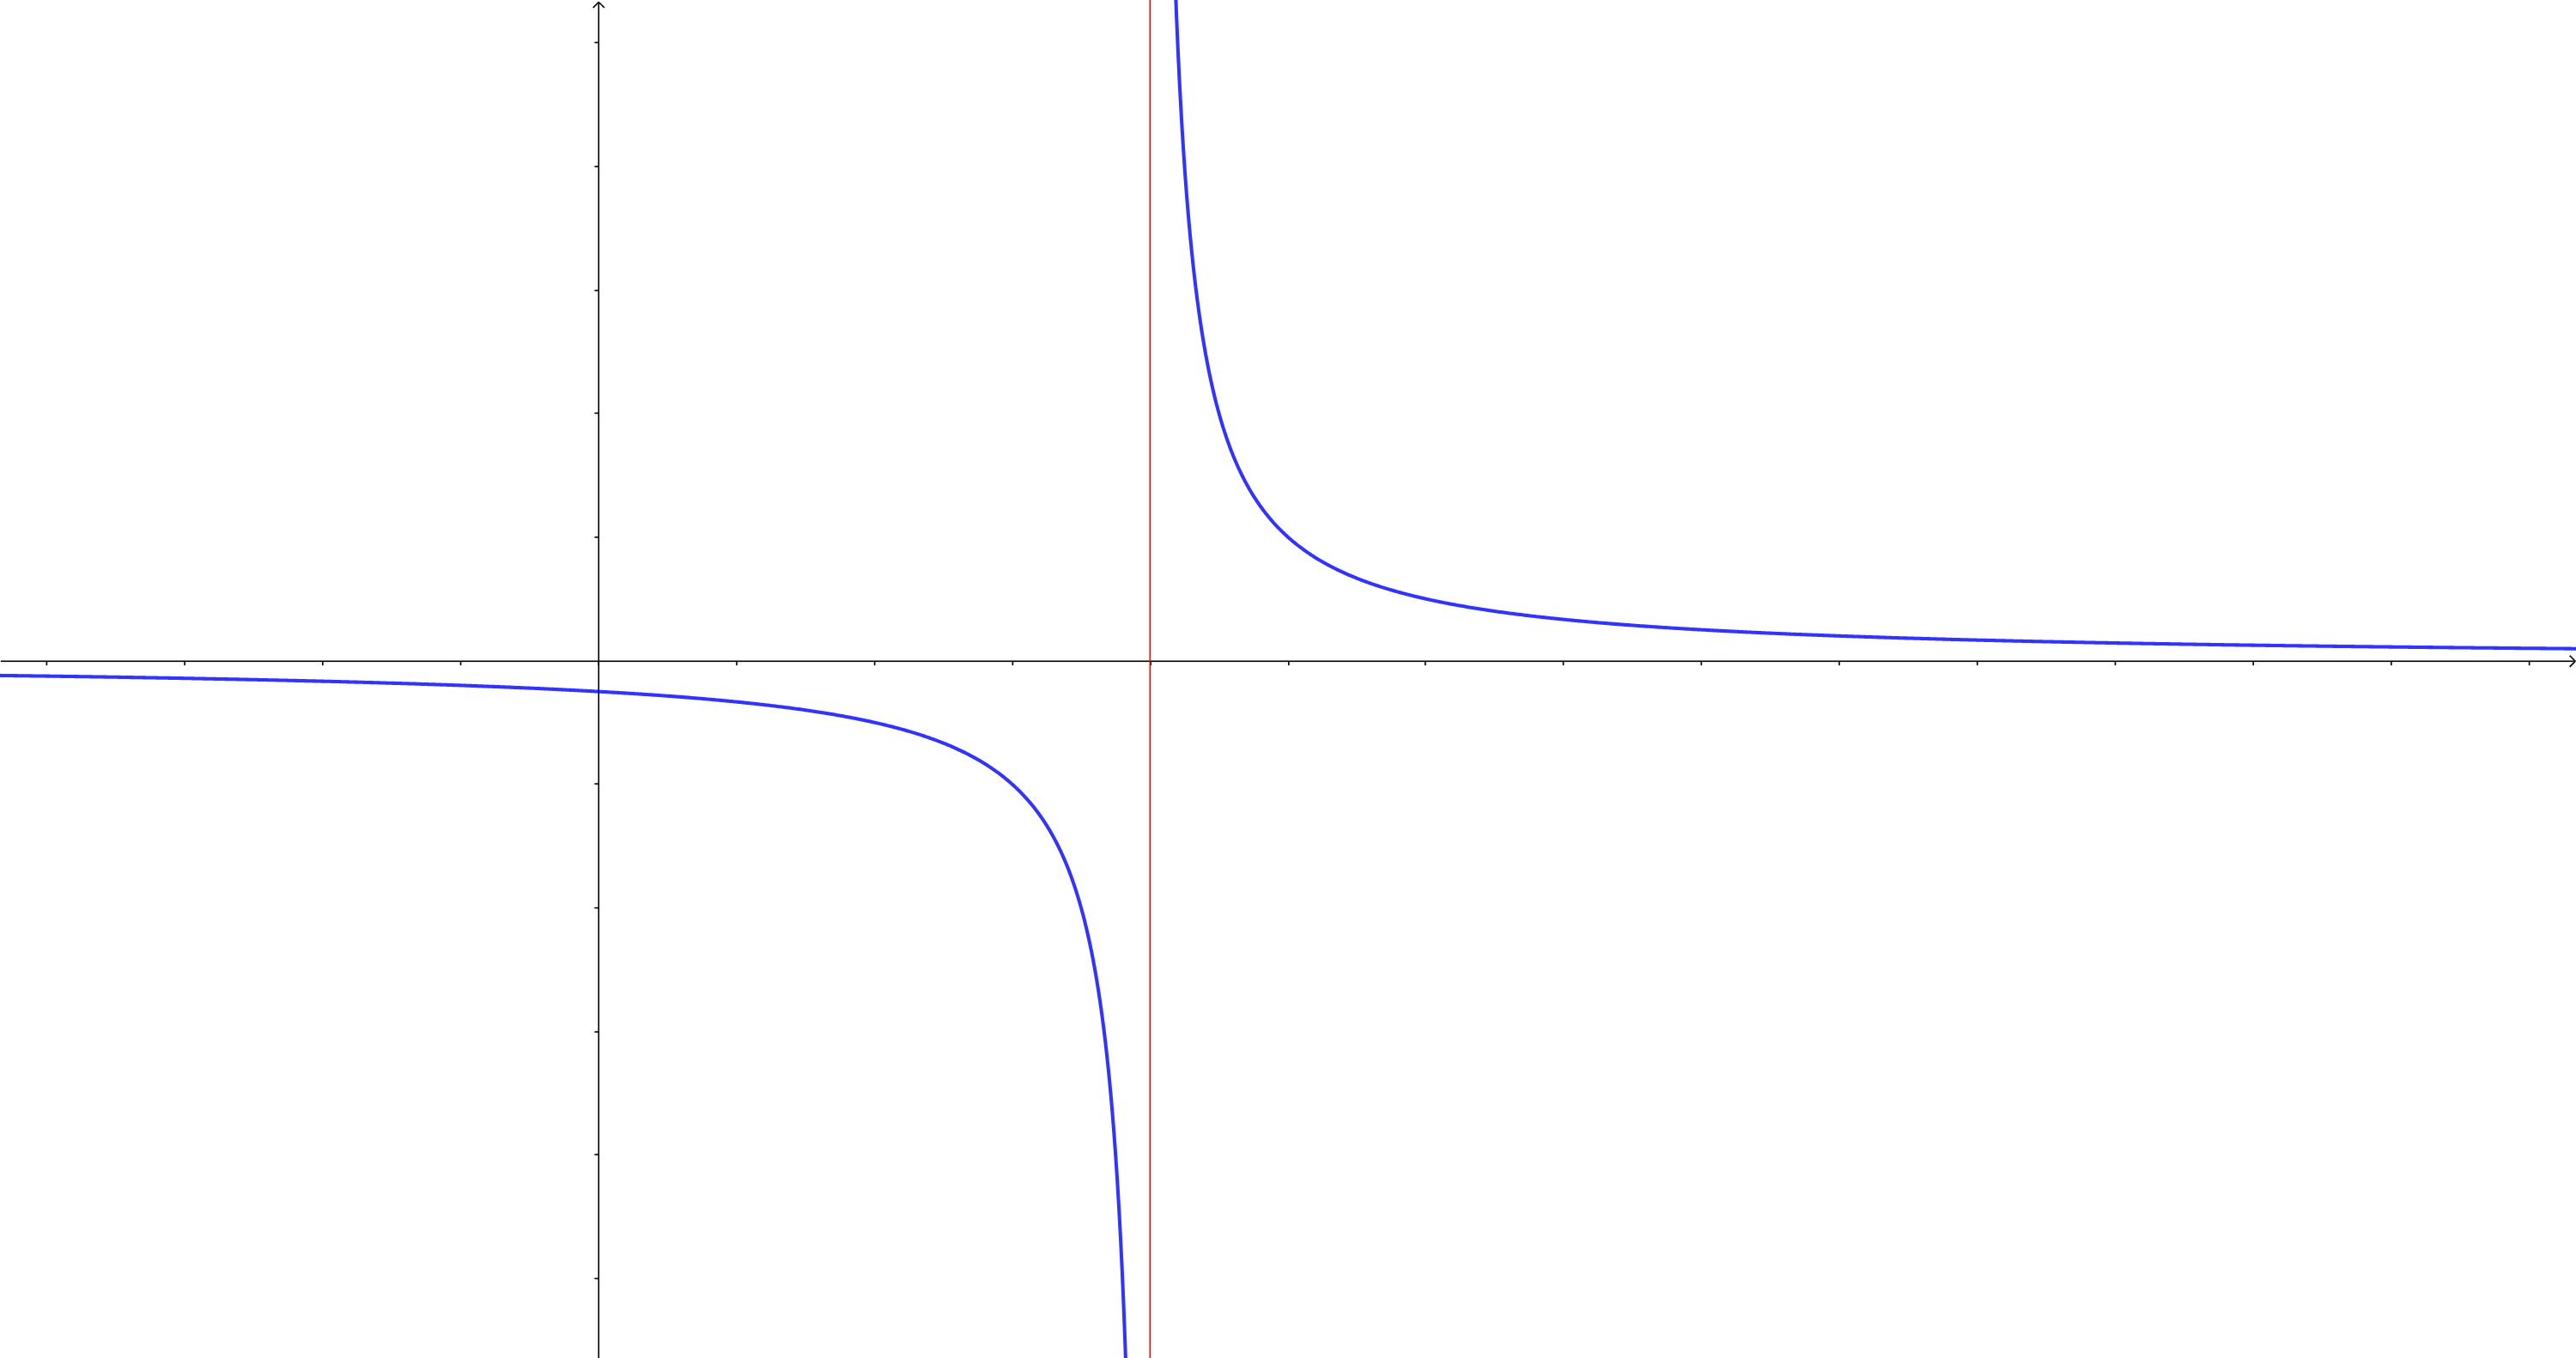
\includegraphics[width=0.6\textwidth, alt={A plot of the reciprocal of (x-2) which tends to zero as x goes to either plus or minus infinity and diverges as x tends to 2.}]{figures/asymptotes}
    \caption{A plot of the function from \cref{eq: reciprocal of x-2} produced using GeoGebra. The blue line is the function and the red line shows where the function diverges and has a vertical asymptote.}
\label{fig: asymptotes function}
\end{figure}

The general rule when curve sketching is to set $y=f(x)$ for the function of interest $f(x)$, and then to investigate the following:
\begin{itemize}
%\setlength{\itemsep}{-5pt}
    \item The \textbf{intercepts} of $f(x)$, these are the points where the function meets or crosses the coordinate axes, e.g. $f(x=0)$ and $f(x)=0$, as these position the graph relative to the coordinate axes.
    \item What happens to $y$ as $x\to\pm\infty$?
   \item Which values of $x$ make $y\to \pm\infty$?
   \item Does the function have any \textbf{symmetry}? For example does $f(-x)=f(x)$ ($f$ is even), or $f(-x)=-f(x)$ ($f$ is odd).
   \item Is the function periodic? 
\end{itemize}
Note that a function can have several of these interesting features. e.g. the trig functions are all periodic, while $\sin(x)$ and $\tan(x)$ are odd functions and $\cos(x)$ is an even function.

\begin{mdiv}
An asymptote to a curve is a straight line that becomes close to the curve as either $x$ or $y$ tend to $\pm\infty$. In our above example the curve of \cref{eq: reciprocal of x-2} has two asymptotes, the horizontal $x$-axis for $x\to \pm\infty$ and the vertical line $x=2$ for $x\to 2$.\\

When sketching a curve it is often useful to start by drawing the asymptotes in as they help you to know how the function will behave in certain regions of the plot. In some books you may see $f(x)\asymp mx +c$ as $x\to \infty$ to signify that the straight line $y=mx+c$ is an asymptote to the graph of $f(x)$ as $x$ tends to infinity.
\end{mdiv}

\begin{exercise}
Apply the above rules to produce a sketch of the function
\begin{equation*}
f(x)=\frac{x+2}{x-1}.
\end{equation*}
\end{exercise}

\begin{ex}
Consider the rational function 
\begin{equation*}
f(x)=\frac{x^{2}+4x-12}{x^{2}-2x}
\end{equation*}
and compute its limit as $x\to 2$.

Looking at the function you may think that it will diverge as $x\to 2$ since the denominator vanishes there. However the first step is always to look at if there are any common factors between the numerator and denominator. Factorising both we have
\begin{align*}
f(x)&=\frac{x^{2}+4x-12}{x^{2}-2x}\\
&=\frac{(x+6)(x-2)}{x(x-2)}\\
&=\frac{x+6}{x}.
\end{align*}
So the denominator does not vanish at $x=2$. We can now evaluate the limit to be
\begin{equation*}
\lim_{x\to 2}f(x)=\lim_{x\to 2}\frac{x+6}{x}=\frac{8}{2}=4.
\end{equation*}

The limit is the same regardless of which direction we approach $2$ from.
\end{ex}

\begin{exercise}
Estimate the limit from the above example by constructing a table of values of $x$ and $f(x)$ for $x$ approaching 2 from both above and below.
\end{exercise}

As a warning, this approach of tabulating the values does not work if the function is oscillating. For example, if you try to evaluate the limit as $x\to 0$ of $\cos\left(\uppi/x\right)$ it can look like it is tending to a constant if we are not careful with the values that we pick. However, if we plot the function we see that it is highly oscillatory around zero.

\begin{ex}
Consider the rational function
\begin{equation*}
f(x)=\frac{x^{3}+x^{2}-5x-2}{2x^{3}-7x^{2}+4x+4}.
\end{equation*}
It has three interesting limits, $x\to 0,\infty,2$. We can evaluate the first two of these here, but need to leave the third, $x\to 2$ until we have learnt about L'H\^{o}pital's rule in \cref{sec:advanced topics}. We will do $x\to 0$ first. As usual we check that the numerator and denominator both make sense as $x\to 0$ and then can evaluate the limit
\begin{align*}
\lim_{x\to 0}f(x)&=\lim_{x\to 0}\frac{x^{3}+x^{2}-5x-2}{2x^{3}-7x^{2}+4x+4}\\
&=\frac{-2}{4}\\
&=-\frac{1}{2}.
\end{align*}

Next we do the $x\to \infty$ limit.  Before we do this we need to multiply $f(x)$ by $x^{-3}/x^{-3}$ so that it becomes
\begin{align*}
\lim_{x\to \infty}f(x)	&=\lim_{x\to \infty}\left(\frac{x^{-3}}{x^{-3}}\frac{x^{3}+x^{2}-5x-2}{2x^{3}-7x^{2}+4x+4}\right)\\
				&=\lim_{x\to \infty}\left(\frac{1+x^{-1}-5x^{-2}-2x^{-3}}{2-7x^{-1}+4x^{-2}+4x^{-3}}\right)\\
				&=\frac{1}{2}.
\end{align*}
\end{ex}

Remember that when evaluating a limit we want to look for as many cancellations as possible to simplify the calculation. This can be looking for common factors between the numerator and denominator, but can also mean fully expanding out all terms as there may be cancellations hidden by the way the function has been written.

Often it is useful to plot a function when we are estimating the limit, while this is not compulsory it can be very helpful, particularly if as in the case of $\tan(x)$, the value of the limit depends on the direction of approach.\\

\begin{figure}[ht]
    \centering
  %  \pdftooltip{
  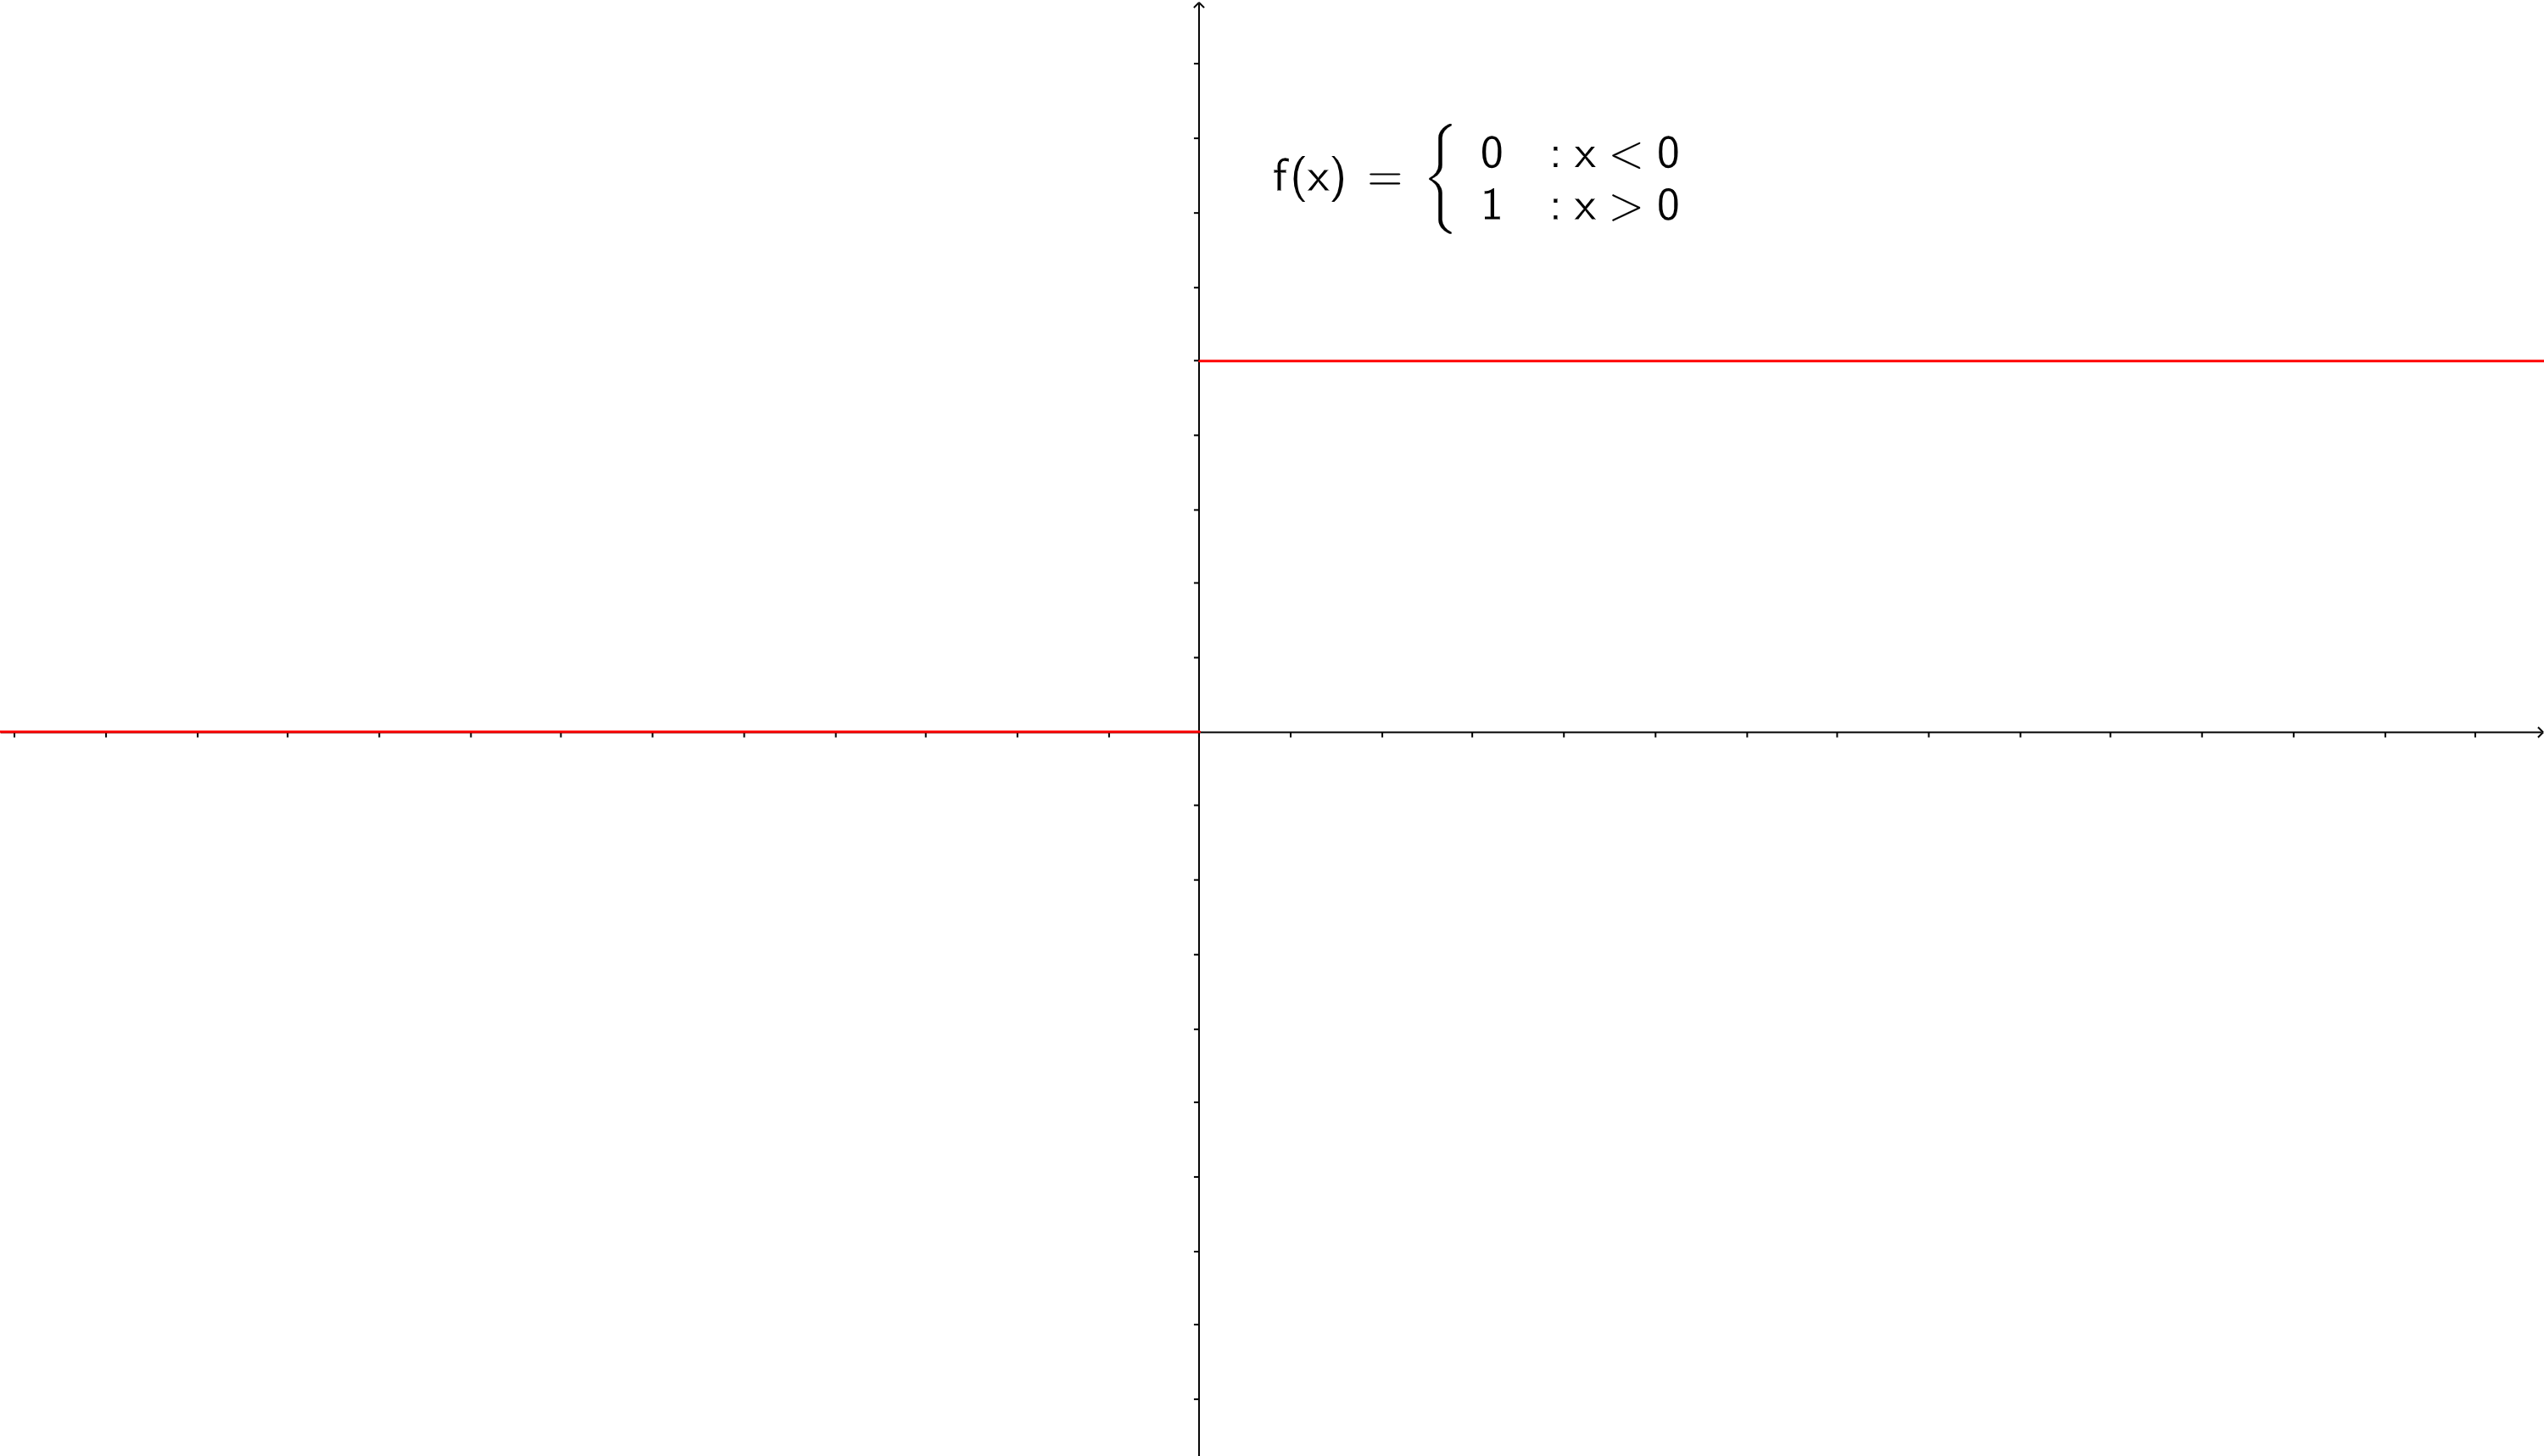
\includegraphics[width=0.5\textwidth,alt={A plot of a step function.}]{figures/step_function}
  %}{A plot of the tan function. }
    \caption{A plot of a step function from \cref{eq: step function} produced using GeoGebra.}
\label{fig: step function}
\end{figure}

\begin{ex}
Consider the step function
\begin{equation}
f(x)=\begin{cases}
&0 \quad x < 0\\
&1 \quad x\geq 0,
\end{cases}
\label{eq: step function}
\end{equation}
shown in \cref{fig: step function}. By looking at the graph we see that the limit of $f(x)$ as $x\to 0$ will depend on the direction of approach. If we start from below zero it is clear that $f(x)\to 0$, while starting above zero it is clear that $f(x)\to 1$. In contrast to the case of $\tan(x)$ the function is not diverging in the limit, but we still end up with a \textbf{One Sided Limit}\footnote{This just means that the function is well behaved in the limit as long as we only look at one side. }
\end{ex} 



\begin{mdiv}
Note that it can be dangerous to use $\infty$ in calculations as if it were a number. This is because there are certain limits and other expressions that we may see which do not make sense:
\begin{equation*}
\infty^{0}, \quad \infty-\infty, \quad \frac{0}{0}, \quad 0^{0}, \quad \frac{\infty}{\infty}, \quad \frac{\infty}{0}, \quad \frac{1}{0}.
\end{equation*}
Just because we see one of these expressions coming out a limit does not necessarily mean that the limit does not exist. It can instead mean that we need to be very careful how we evaluate the limit. In \cref{sec:advanced topics} we will discuss L'H\^{o}pital's rule which is a techniques for evaluating limits that initially look like they do not make sense.
\end{mdiv}

There are a few limits that we need to know that we will not prove here, time permitting we will prove these in \cref{sec:advanced topics}, but you can also look at the ``Proof of Trig Limits'' section of \cite{calcI} to see one approach to proving them. These limits are
\begin{align}
\lim_{x\to 0}\frac{\sin x}{x}&=1, \label{eq: sin limit}\\
\lim_{x\to 0}\frac{\cos x -1}{x}&=0, \label{eq: cos limit}\\
\lim_{h\to 0}\frac{e^{h}-1}{h}&=1, \label{eq: exp limit}\\
\lim_{h\to 0}\frac{\ln(1+h)}{h}&=1. \label{eq: ln limit}
\end{align}
Note that \cref{eq: exp limit} is equivalent to \cref{eq: exp approximation} which we discussed above as one of the definitions of the exponential function.

\section{Continuity and differentiability}
\label{sec: continuity}
Now that we have some examples of functions and understand how to take limits, we can define two properties of a function which will be very important later in the course: \textbf{continuity} and \textbf{differentiability}. \\

A function $f(x)$ is said to be continuous at a point $x=a$ if
\begin{equation}
\lim_{x\to a}f(x)=f(a).
\label{eq: continuity}
\end{equation}

If $X$ is the domain of $f(x)$, we say that $f$ is continuous on $X$ if it is continuous at each point in $X$, often we would just say that $f$ is a continuous function. As a rule of thumb, we can say that a function is continuous if its graph can be drawn from start to finish without taking your pen off the paper. Functions which are not continuous will have jumps or divergences at the point that fails to be continuous.\\

If we have a rational function then we can find where it is not continuous, called being \textbf{discontinuous}, by finding the roots of the denominator.\\

\begin{mdiv}
If we are being careful we need to give three parts to the definition of continuity: 
\begin{itemize}
%\setlength{\itemsep}{-5pt}
    \item[1)] The limit of $f(x)$ as $x\to a$ exists.
    \item[2)] The value of $f(x)$ is defined at $x=a$. i.e. $f(a)$ is defined and is finite.
   \item[3)] The limit of $f(x)$ as $x\to a$ agrees with the value of $f(a)$.
\end{itemize}
This is another place where as this is not a course for mathematicians we can combine all three of these into the one statement in \cref{eq: continuity}. This is another example of being able to use a working definition and not needing to get sidetracked by all of the technical details.
\end{mdiv}

\begin{ex}
We have already met several examples of continuous and discontinuous functions:
\begin{itemize}
%\setlength{\itemsep}{-5pt}
    \item The trig functions $\cos(x)$ and $\sin(x)$ are continuous on all of $\R$.
    \item The exponential function $\exp(x)$ is continuous on all of $\R$.
   \item The natural logarithm is continuous on the positive real numbers $\R$ as, currently we have not defined it for negative $x$, and it diverges in the limit $x\to 0$.
   \item The tangent function $\tan(x)$ are not continuous on $\R$ due to its divergences at $\pm\frac{\uppi}{2},\pm\frac{3\uppi}{2},\dots{}$. However, it is continuous on its domain\footnote{Strictly speaking this is the principle domain of $\tan(x)$ its domain is really $\{x\in \R\vert x\neq \uppi/2 +n\uppi, n\in \Z\}$} $\left(-\frac{\uppi}{2},\frac{\uppi}{2}\right)$
   \item The step function of \cref{eq: step function} is not continuous at $x=0$.
\item The function in \cref{eq: reciprocal of x-2} has a discontinuity at $x=2$
\end{itemize}
\end{ex}
\begin{exercise}
Use the definition of continuity to determine if the function
\begin{equation}
g(x)=\frac{4x+10}{x^{2}-2x-15}
\end{equation}
is continuous and if not find the points where it has discontinuities.
\end{exercise}

Related to continuity is differentiability. A function $f(x)$ is differentiable at a point $a$ if the limit
\begin{equation*}
\lim_{x\to a}\frac{f(x)-f(a)}{x-a}
\end{equation*}
exists. We call this limit the derivative of the function at the point $a$,
\begin{equation}
f'(a)=\lim_{x\to a}\frac{f(x)-f(a)}{x-a},
\label{eq: rate of change at a}
\end{equation}
the notation $\frac{\ud f}{\ud x}(a)$ is sometimes used instead of $f'(a)$. A function is called continuously differentiable if its derivative is also continuous.\\

It is important to note that differentiability at $a$ implies continuity at $a$, but continuity does not imply differentiability.  For example the absolute value function shown in \cref{fig: abs function} is continuous everywhere, but is only differentiable everywhere except at $x=0$.

\begin{figure}[htbp]
    \centering
\ThisAltText{Graph of the absolute value function.}
%    \pdftooltip{
    \begin{tikzpicture}[line width=1pt,line cap=round,line join=round,domain=-2.5:2.5, smooth,variable=\x]
     \draw[->] (-3,0) -- (3.3,0) node[above] {$x$};
  \draw[->] (0,-0.2) -- (0,3) node[above] {$y$};
 \draw[color=red]   plot (\x,{abs(\x)}) node[right] {$f(x)=\vert x\vert$};
    \end{tikzpicture}
%    }{absolute value function}
    \caption{The absolute value function $f(x)=\vert x\vert$ is continuous at every point, but it is not differentiable at the point $x=0$.}
        \label{fig: abs function}
\end{figure}

\begin{ex}
Consider the modulus or absolute value function shown in \cref{fig: abs function}. We have said that this is a continuous function which is not differentiable at $x=0$, but how do we show this? We do it by checking all of the limits.\\

Checking continuity at $x=0$ is left as an exercise. For differentiability we need to check the limits as $x\to 0^{+}$ and $x\to 0^{-}$. 

In the first one we have:
\begin{equation*}
\lim_{x\to 0^{+}}\frac{f(x)-f(0)}{x}=\lim_{x\to 0^{+}}\frac{x-0}{x}\lim_{x\to 0^{+}}1=1,
\end{equation*}
while approaching from the other direction gives:
\begin{equation*}
\lim_{x\to 0^{-}}\frac{f(x)-f(0)}{x}=\lim_{x\to 0^{-}}\frac{(-x)-0}{x}\lim_{x\to 0^{-}}-1=-1.
\end{equation*}
These do not agree, so the limit does not exist and the modulus function is not differentiable.
\end{ex}

\begin{figure}[ht]
    \centering
    %\pdftooltip{
\ThisAltText{Graph of a straight line function.}
\begin{tikzpicture}[line width=1pt,line cap=round,line join=round]
\draw[black, ultra thick,->] (0,0) --(5,0) node[anchor=west]{$x$ axis};
\draw[black, ultra thick,->] (0,0) --(0,5) node[anchor=south]{$y$ axis};
%\draw[step=1cm,gray,very thin] (-2,-2) grid (6,6);
%\draw[blue, ultra thick] (0,0) parabola (6,6);
\draw[red, ultra thick] (0,0) -- (5,5);
 \filldraw[black] (2,2) circle (2pt) node[right,xshift=3mm]{$y_{1}$ at $x_{1}$};
 \filldraw[black] (4,4) circle (2pt) node[right,xshift=3mm]{$y_{2}$ at $x_{2}$};
\end{tikzpicture}
%}{A displacement time graph showing the difference between constant velocity motion and motion with a changing velocity.}
    \caption{A plot of the straight line $y=x$ and example of $y=mx+c$ with gradient $m=1$ and $y$-intercept $c=0$, with two points on the line marked.}
    \label{fig: straight line graph.}
\end{figure}

The fraction in \cref{eq: rate of change at a} may look familiar to you. If we had a straight line $y=f(x)=mx+c$ where $m$ is the gradient of the straight line and $c$ is the $y$-intercept, then calculating this fraction gives
\begin{equation*}
\frac{f(x)-f(a)}{x-a}=\frac{mx+c-(ma+c)}{x-a}=\frac{m(x-a)}{x-a}=m,
\end{equation*}
which is the gradient of the curve. For a function that is not a straight line, this procedure gives the gradient of the straight line between $x$ and $a$. In the limit that $x\to a$ this fraction becomes the gradient of the \textbf{tangent} line\footnote{A tangent is a line that touches a curve at one point} to the curve at $a$.   See \cref{fig: parabola tangent} for the example of the tangent to parabola $y=x^{2}$.


\begin{mdiv}
The fraction
\begin{equation*}
\frac{f(x)-f(a)}{x-a}
\end{equation*}
is sometimes referred to as the Newton quotient of the function $f(x)$ at the point $a$. This is after Isaac Newton because when calculating a derivative we are calculating this quotient for smaller and smaller differences $x-a$.
\end{mdiv}

\begin{figure}[ht]
    \centering
\ThisAltText{Graph of a parabola with a tangent curve shown .}
\begin{tikzpicture}[line width=1pt,line cap=round,line join=round]
    \begin{axis}[
            xtick = \empty,    ytick = \empty,
            xlabel = {$x$},
            x label style = {at={(1,0)},anchor=west},
            ylabel = {$y$},
            y label style = {at={(0,1)},rotate=-90,anchor=south},
            axis lines=left,
            enlargelimits=0.2,
        ]
        \addplot[color=black,smooth,thick,-] {(x)^2};
        \addplot[mark=none, red] coordinates {(-6,20) (0,-4)};
    \end{axis}
\end{tikzpicture}
 \caption{A plot of a parabola in black and its tangent in red}
    \label{fig: parabola tangent}
\end{figure}
\newpage

%%%%%%%%%%%%%%%%%%%%%%%%%%%%%%%%%%%%%%%%%%%%%%


\chapter{Differentiation}
\label{sec:differentiation}
\epigraph{You take a function of $x$ and you call it $y$.\\ Take any $x_{0}$ that you care to try.\\ You make a little change and call it $\Delta x$.\\ The corresponding change in $y$ is what you find next. }{\textit{The Derivative Song by Tom Lehrer}}

\section{Differentiation from first principles}
In the previous \namecref{sec:functions}, we encountered the derivative of a function at a point in \cref{eq: rate of change at a} and its interpretation as the tangent to a curve at the point $a$. With a small amount of rewriting, setting $x=a+h$ for $x$ ``near'' $a$, this becomes
\begin{align*}
f'(a)&=\lim_{x\to a}\frac{f(x)-f(a)}{x-a}\\
&=\lim_{h\to 0}\frac{f(a+h)-f(a)}{a+h-a}\\
&=\lim_{h\to 0}\frac{f(a+h)-f(a)}{h}.
\end{align*} 
This is still an expression for the tangent to a curve at a specific point $x=a$. However, if we are interested in the gradient at an arbitrary point $x$, then we can rewrite it as
\begin{equation}
f'(x)=\lim_{h\to 0}\frac{f(x+h)-f(x)}{h}.
\label{eq: derivative definition}
\end{equation}

The formula in \cref{eq: derivative definition} is the definition of the \textbf{derivative} of the function $f(x)$. Not that only functions where the derivative exists for all points are called \textbf{differentiable}. There is a range of notation\footnote{We will only use the two most common notations in this course. However, another notation that you may see in books is $f_{x}(x)$, where the subscript shows what we are differentiating with respect to. This notation shows up a lot if we have functions of more than one variable where we need to make it clear which variable we are differentiating with respect to. In the assessed part of this course we will only care about functions of one variable so do not need this notation.} and terminology used to denote derivative. The notation used above,  $f'(x)$ is known as the \textbf{Lagrange} or \textbf{Euler} notation\footnote{In an example of Sigler's law of eponymy, this is most commonly called Lagrange's notation even though it was first used by Euler. It is also quite close to the original notation that Newton used when he discovered calculus and referred to it as the \textbf{method of fluxions}. }.  The other very common notation is due to \textbf{Leibniz} where we write
\begin{equation}
\frac{\ud f}{\ud x}=\lim_{h\to 0}\frac{f(x+h)-f(x)}{h},
\label{eq: Leibniz definition}
\end{equation}
this notation is particularly useful when we learn about integration as in certain contexts we can treat the derivative like a fraction.\\

\begin{mdiv}
In \cref{eq: Leibniz definition} it looks like the right hand side is a fraction. This is not true, other than in certain very specific circumstances, we will not see $\ud f$ or $\ud x$ appearing on their own. In Newton's approach the Newton quotient is sometimes written as
\begin{equation*}
\frac{\Delta f}{\Delta x}=\frac{f(x)-f(a)}{x-a},
\end{equation*}
which does make sense as a fraction. The limit where this becomes the derivative is when the change in $x$, $\Delta x=x-a$, goes to zero. In this limit if we really had a fraction it would look like $0/0$, which is one of the nonsense expressions that we mentioned earlier. The power of calculus is that it enables us to make sense of this limit, but what we loose is the ability to treat it as a fraction. When we discuss integration and differential equations later on in the module we will return to this idea.
\end{mdiv}

If we use \cref{eq: derivative definition} to calculate the derivative of a function this is called \textbf{differentiation by first principles}. As you might expect, when the function $f(x)$ becomes more complicate calculating the derivative in this way becomes more complicated as well. Fortunately, there are certain standard rules and techniques that we can learn to simplify matters. With a little work all of these can be proved from the definition of the derivative, some of these proofs will be given here but others are left as an exercise to the interested reader.\\

As a warm up we will use \cref{eq: derivative definition} to calculate the derivative of a straight line.
\begin{ex}
Consider $f(x)=mx+c$ and calculate the derivative from first principles:
\begin{align*}
f'(x)	&=\lim_{h\to 0}\frac{f(x+h)-f(x)}{h}\\
	&=\lim_{h\to 0}\frac{m(x+h)+c-(mx+c)}{h}\\
	&=\lim_{h\to 0}\frac{mx+mh+c-mx-c}{h}\\
	&=\lim_{h\to 0}m\frac{h}{h}\\
	&=\lim_{h\to 0}m=m.
\end{align*}
So derivative of a straight lime is a constant, the gradient of the line. We already knew this, but it is a good consistency check to ensure that our definition of the derivative is working as expected.
\end{ex}

\begin{ex}
Consider the function $f(x)=4x^2 -6x +2$, using \cref{eq: derivative definition} we calculate its derivative as follows:
\begin{align*}
f'(x)	&=\lim_{h\to 0}\frac{f(x+h)-f(x)}{h}\\
	&=\lim_{h\to 0}\frac{4(x+h)^2 -6(x+h) +2)-(4x^2 -6x +2)}{h}\\
	&=\lim_{h\to 0}\frac{4(x^{2}+2xh+h^{2})-6x-6h+2-4x^{2}+6x-2}{h}\\
	&=\lim_{h\to 0}\frac{8xh+4h^{2}}{h}\\
	&=\lim_{h\to 0}\left(8x+4h\right)=8x.
\end{align*}
Notice that since the curve is no longer a straight line the derivative , and thus the gradient of the tangent to the curve, depends where the point is along the curve. 
\end{ex}

Remember that if the limit in \cref{eq: derivative definition} does not exist at a particular value of $x$, then the derivative does not exist. In other words, the definition of the derivative only makes sense for functions which satisfy the condition of differentiability.

\begin{ex}
Consider the function 
\begin{equation*}
g(x)=\frac{1}{x+1},
\end{equation*}
and calculate its derivative. Note that this function has a discontinuity at $x=-1$ so it will not be differentiable at that point.\\

Calculating $g'(x)$ is good practice as we need to be careful when we have fractions.
\begin{align*}
g'(x)	&=\lim_{h\to 0}\frac{g(x+h)-g(x)}{h}\\
	&=\lim_{h\to 0}\frac{1}{h}\left(\frac{1}{x+h+1}-\frac{1}{x+1}\right)\\
	&=\lim_{h\to 0}\frac{1}{h}\left(\frac{x+1}{(x+h+1)(x+1)}-\frac{x+h+1}{(x+1)(x+h+1)}\right)\\
	&=\lim_{h\to 0}\frac{1}{h}\left(\frac{x+1-x-h-1}{(x+h+1)(x+1)}\right)\\
	&=\lim_{h\to 0}\frac{1}{h}\left(\frac{-h}{(x+h+1)(x+1)}\right)\\
	&=\lim_{h\to 0}\frac{-1}{(x+h+1)(x+1)}\\
	&=-\frac{1}{(x+1)^{2}}.
\end{align*}
\end{ex}

We can also calculate the derivatives of some of the special functions from first principles.
\begin{ex}
Consider $f(x)=\sin(x)$, this is a continuous function so we can hope that the derivative exists. Note that we can use the addition formula for $\sin(x)$ to expand $\sin(x+h)$ as
\begin{equation*}
\sin(x+h)=\sin(x)\cos(h)+\sin(h)\cos(x).
\end{equation*}
Thus \cref{eq: derivative definition} becomes
\begin{align*}
f'(x)	&=\lim_{h\to 0}\frac{f(x+h)-f(x)}{h}\\
	&=\lim_{h\to 0}\frac{\sin(x+h)-\sin(x)}{h}\\
	&=\lim_{h\to 0}\frac{\sin(x)\cos(h)+\sin(h)\cos(x)-\sin(x)}{h}\\
	&=\lim_{h\to 0}\left(\sin(x)\frac{\cos(h)-1}{h}+\cos(x)\frac{\sin(h)}{h}\right)\\
	&=\sin(x)\lim_{h\to 0}\frac{\cos(h)-1}{h}+\cos(x)\lim_{h\to 0}\frac{\sin(h)}{h}\\
	&=\cos(x),
\end{align*}
where we have used the trig limits from \cref{eq: sin limit,eq: cos limit}
\end{ex}

\begin{exercise}
Show that the derivative of $f(x)=\cos(x)$ is $f'(x)=-\sin(x)$ using differentiation from first principles.
\end{exercise}

\begin{ex}
Consider $f(x)=e^{x}$, its derivative is
\begin{align*}
f'(x)	&=\lim_{h\to 0}\frac{f(x+h)-f(x)}{h}\\
	&=\lim_{h\to 0}\frac{e^{x+h}-e^{x}}{h}\\
	&=\lim_{h\to 0}\frac{e^{x}e^{h}-1}{h}\\
	&=e^{x}\lim_{h\to 0}\frac{e^{h}-1}{h}\\
	&=e^{x}.
\end{align*}
Where we use \cref{eq: exp limit} to evaluate the limit in the final line. This result that the derivative of $e^{x}$ is equal to $e^{x}$, is sometimes taken to be a definition of the exponential function. 
\end{ex}

The other standard derivative that you need to know is the derivative of the natural logarithm.
\begin{ex}
Consider $f(x)=\ln(x)$, we calculate its derivative as
\begin{align*}
f'(x)	&=\lim_{h\to 0}\frac{f(x+h)-f(x)}{h}\\
	&=\lim_{h\to 0}\frac{\ln(x+h)-\ln(x)}{h}\\
	&=\lim_{h\to 0}\frac{1}{h}\ln\left(\frac{x+h}{x}\right)\\
	&=\lim_{h\to 0}\frac{1}{h}\ln\left(1+\frac{h}{x}\right),
\end{align*}
now we can let  $\epsilon =h/x$ which is tending to zero as $h$ tends to zero. Thus the derivative becomes
\begin{align*}
f'(x)	&=\lim_{\epsilon\to 0}\frac{1}{x\epsilon}\ln\left(1+\epsilon\right)\\
	&=\frac{1}{x}\lim_{\epsilon\to 0}\frac{\ln\left(1+\epsilon\right)}{\epsilon}\\
	&=\frac{1}{x},
\end{align*}
where we have made use of \cref{eq: ln limit}
\end{ex}

Using the first principles definition to calculate derivatives is hard work and involves careful manipulation of limits. You will be please to know that we will only use it in certain relatively simple cases. For more complicated expressions we can use a range of other techniques and formulas. Eventually you will internalise some of the standard derivative expressions or use a formula sheet like that in \cref{sec: deriv sheet}.

%\section{Standard derivatives}


\section{Differentiation techniques}

\subsection*{Properties of the derivative}
In this section we will see the various formulae and rules in both the Lagrange and Leibniz notation so you should be familiar with both and use the notation that you feel most comfortable with.\\

The first thing that we need is to know is how to differentiate the sum of two functions and the product of a function with a number.  The proof of these results will be given in \cref{sec: proofs}. These formulae are:
\begin{align}
\frac{\ud}{\ud x}\left(f(x)+g(x)\right)	&=\frac{\ud f(x)}{\ud x}+\frac{\ud g(x)}{\ud x}, \label{eq: derivative of sum}\\
\frac{\ud}{\ud x}\left(f(x)-g(x)\right)	&=\frac{\ud f(x)}{\ud x}-\frac{\ud g(x)}{\ud x}, \label{eq: derivative of difference}\\
\frac{\ud}{\ud x}\left(cf(x)\right)	&=c\frac{\ud f(x)}{\ud x},\label{eq: derivative scalar multiplication}
\end{align}
where $c$ is any number.\\

In the Lagrange/Euler notation these formulae are:
\begin{align}
\left(f(x)+g(x)\right)'	&=f'(x)+g'{x}, \label{eq: derivative of sum 2}\\
\left(f(x)-g(x)\right)'&=f'(x)-g'(x), \label{eq: derivative of difference 2}\\
\left(cf(x)\right)'	&=cf'(x). \label{eq: derivative scalar multiplication 2}
\end{align}

These are useful formulae that we will frequently use in calculations as it enables us to split up the functions that we are differentiating into smaller tractable parts. The other shortcuts that we have is that the derivative of a constant is zero,
\begin{equation}
\frac{\ud c}{\ud x}=0, \label{eq: derivative of constant}
\end{equation}
and that the derivative of a \textbf{monomial} is
\begin{equation}
\frac{\ud}{\ud x}\left(x^{n}\right)=nx^{n-1}. \label{eq: monomial derivative}
\end{equation}
Sometimes the second formula is referred to as the \textbf{power rule}, and is one of the most important rules that you can learn as it enables you to differentiate any polynomial.\\

The formula in \cref{eq: derivative of constant}, which says that the derivative of a constant is zero makes sense since the derivative measures the rate of change of a function. A constant is, by definition, not changing so its rate of change is zero.\\

We can now use these rules to calculate some example derivatives.
\begin{ex}
Consider the function 
\begin{equation*}
f(x)=15x^{20}-3x^{5}+2x+4.
\end{equation*}
We calculate its derivative as follows:
\begin{align*}
\frac{\ud f}{\ud x}	&=\frac{\ud}{\ud x}\left(15x^{20}-2x^{5}+2x+4\right)\\
			&=15\frac{\ud}{\ud x}\left(x^{20}\right)-2\frac{\ud}{\ud x}\left(x^{5}\right)+2\frac{\ud}{\ud x}\left(x\right)+\frac{\ud}{\ud x}\left(4\right)\\
			&=15 \times 20 x^{19}-2\times 5 x^{4}+2 +0\\
			&=300 x^{19}-10x^{4}+2.
\end{align*}
\end{ex}

\begin{ex}
Consider the function 
\begin{equation*}
g(x)=\frac{6}{x^{2}}-4x^{2}+2x.
\end{equation*}
Its derivative is calculated as follows 
\begin{align*}
\frac{\ud g}{\ud x}	&=\frac{\ud}{\ud x}\left(\frac{6}{x^{2}}-4x^{2}+2x\right)\\
			&=6\frac{\ud}{\ud x}\left(x^{-2}\right)-4\frac{\ud}{\ud x}\left(x^{4}\right)+2\frac{\ud }{\ud x}\left(x\right)\\
			&=6\times (-2) x^{-3}-4\times 4 x^{3}+2\\
			&=-\frac{12}{x^{3}}-16x^{3}+2.
\end{align*}
\end{ex}

\begin{exercise}
Calculate the derivative of 
\begin{equation*}
y=8x^{2}+2x-\frac{1}{x}.
\end{equation*}
\end{exercise}

\subsection*{Product rule}
So far we have not discussed differentiating the product of two functions, unless you count $x^{a+b}=x^{a}x^{b}$. A very useful formula is the \textbf{Leibniz} or \textbf{product rule} which tells us how to differentiate the product of two functions. The product rule is
\begin{equation}
\frac{\ud }{\ud x}\left(f(x)g(x)\right)=\frac{\ud f}{\ud x}g(x)+f(x)\frac{\ud g}{\ud x}. \label{eq: product rule}
\end{equation}

You may think that it is disappointing that the derivative of a product is not just the product of the derivatives. However, you will come to appreciate the product rule as you make use of it. It will become particularly useful once we have discussed more about how to differentiate trig functions and exponentials. 

\begin{ex}
For the product of two functions $\sqrt{x^{3}}\sin(x)$ we find the derivative as follows. Let $f(x)=\sqrt{x^{3}}$ and $g(x)=\sin(x)$ and calculate the individual derivatives to be
\begin{equation*}
f'(x)=(x^{\frac{3}{2}})'=\frac{3}{2}x^{\frac{3}{2}-1}=\frac{3}{2}\sqrt{x}, \qquad g'(x)=(\sin(x))'=\cos(x).
\end{equation*}
Then we use product rule to calculate
\begin{align*}
\left(\sqrt{x^{3}}\sin(x)\right)'	&=\left(f(x)g(x)\right)'\\
					&=f'(x)g(x)+f(x)g'(x)\\
					&=\frac{3}{2}\sqrt{x}\sin(x)+\sqrt{x^{3}}\cos(x).
\end{align*}
\end{ex}

\begin{ex}
We can use the product rule to calculate the derivative of $f(x)=\sin^{2}(x)$. In this case the two functions are the same so we can evaluate the derivative as follows
\begin{align*}
f'(x)	&=\left(\sin^{2}(x)\right)'\\
	&=2\sin(x)\left(\sin(x)\right)'\\
	&=2\sin(x)\cos(x)\\
	&=\cos(2x),
\end{align*}
where we have used one of the trig double angle identities in the last line.
\end{ex}

\begin{exercise}
Use the product rule to calculate the derivative of 
\begin{equation*}
f(x)g(x)=e^{x}\sin(x).
\end{equation*}
\end{exercise}

Note that the product rule applies if we have the product of more than two functions, we just have to iterate it for each pair of functions.

\subsection*{Quotient rule}
If instead of a product of functions we have the ratio of two functions then there is a rule for that, the \textbf{quotient} rule\footnote{You may be looking at these two formula and thinking that we could just use the product rule with $f(x)$ and $(g(x))^{-1}$. If you do this you will get an answer that looks just like the quotient rule. There are some technical differences between this approach and the quotient rule we give here, but as we are not mathematicians here we do not need to worry about them. }. In Leibniz notation the quotient rule is 
\begin{equation}
\frac{\ud }{\ud x}\left(\frac{f(x)}{g(x)}\right)=\frac{\frac{\ud f}{\ud x}g(x)-f(x)\frac{\ud g}{\ud x}}{g^{2}(x)}. \label{eq: quotient rule}
\end{equation}

Remember that in most circumstances you can use either the product rule or the quotient rule, it depends how you want to approach the problem.\\

\begin{ex}
Consider the function
\begin{equation*}
F(x)=\frac{\sin(x)}{e^{x}}.
\end{equation*}
Note that we could use the product rule on $e^{-x}\sin(x)$ but will instead use the quotient rule here. Spilt $F(x)$ into the two functions $f(x)=\sin(x)$ and $g(x)=e^{x}$, applying the quotient rule \cref{eq: quotient rule} gives
\begin{align*}
\frac{\ud }{\ud x}\left(\frac{f(x)}{g(x)}\right)&=\frac{\frac{\ud f}{\ud x}g(x)-f(x)\frac{\ud g}{\ud x}}{g^{2}(x)}\\
							&=\frac{e^{x}\cos(x)-\sin(x)e^{x}}{e^{2x}}\\
							&=e^{-x}\left(\cos(x)-\sin(x)\right).
\end{align*}
\end{ex}

\begin{ex}
Consider 
\begin{equation*}
F(x)=\frac{1}{\sin^{2}(x)},
\end{equation*}
and split it into two functions $f(x)=1$ and $g(x)=\sin^{2}(x)$, which have derivatives
\begin{equation*}
\frac{\ud f}{\ud x}=0, \qquad \frac{\ud g}{\ud x}=2\sin(x)\cos(x)=\sin(2x).
\end{equation*}
The quotient rule thus gives that
\begin{align*}
\frac{\ud }{\ud x}\left(\frac{f(x)}{g(x)}\right)&=\frac{\frac{\ud f}{\ud x}g(x)-f(x)\frac{\ud g}{\ud x}}{g^{2}(x)}\\
							&=\frac{0-2\sin(x)\cos(x)}{\sin^{4}(x)}\\
							&=-2\frac{\cot(x)}{\sin^{2}(x)}\\
							&=-2\cot(x)\csc^{2}(x).
\end{align*}
\end{ex}

\subsection*{Derivatives of trig functions}
Armed with the quotient rule we can now give the derivatives of the six trig functions
\begin{align}
\frac{\ud}{\ud x}\sin(ax)&=a\cos(ax),\label{eq: sine derivative}\\
\frac{\ud}{\ud x}\cos(ax)&=-a\sin(ax),\label{eq: cos derivative}\\
\frac{\ud}{\ud x}\tan(ax)&=a\sec^{2}(ax),\label{eq: tan derivative}\\
\frac{\ud}{\ud x}\cot(ax)&=-a\csc^{2}(ax),\label{eq: cot derivative}\\
\frac{\ud}{\ud x}\sec(ax)&=a\sec(ax)\tan(ax), \label{eq: sec derivative}\\
\frac{\ud}{\ud x}\csc(ax)&=-a\csc(ax)\cot(ax).\label{eq: csc derivative}
\end{align}

We have seen how to prove two of these and can now calculate the derivative of $\tan(x)$ the other three will be left as exercises.
\begin{ex}
Consider $f(x)=\tan(x)$, which can be expressed as
\begin{equation*}
f(x)=\tan(x)=\frac{\sin(x)}{\cos(x)}.
\end{equation*}
Using the quotient rule we have that
\begin{align*}
\frac{\ud}{\ud x}\tan(x)	&=\frac{\ud }{\ud x}\left(\frac{\sin(x)}{\cos(x)}\right)\\
				&=\frac{1}{(\cos(x))^{2}}\left(\cos(x)\frac{\ud }{\ud x}\sin(x)-\sin(x)\frac{\ud }{\ud x}\cos(x)\right)\\
				&=\frac{1}{\cos^{2}(x)}\left(\cos(x)\cos(x)-\sin(x)(-\sin(x))\right)\\
				&=\frac{1}{\cos^{2}(x)}\left(\cos^{2}(x)+\sin^{2}(x)\right)\\
				&=\frac{1}{\cos^{2}(x)}\\
				&=\sec^{2}(x).
\end{align*}
Where we have used the identity that $\cos^{2}(x)+\sin^{2}(x)=1$ and the definition of $\sec(x)=1/\cos(x)$.
\end{ex}

\begin{exercise}
Compute the derivatives of $\cot(x), \sec(x),\csc(x)$.
\end{exercise}

\subsection*{Chain rule}
If we have a function of a function, e.g. $f(x)=\exp\left(x^{2}+x\right)$ or $g(x)=\cos\left(x+c\right)$, none of the rules that we have given so far will work. We could go back to first principles, which is exactly what we did when calculating the derivative of $1/(x+1)$, but this would mean that we had to do lots of long and tricky calculations. Fortunately this is not necessary.\\

Consider the function
\begin{equation}
f(x)=\sqrt{4x+2},
\label{eq: function of a function1}
\end{equation}
we can write this as the \textbf{composition} of two functions if we think of $g(x)=\sqrt{x}$ and $h(x)=4x+2$,
\begin{equation*}
f(x)=\left(g\circ h\right)(x)=g(h(x))=g\left(4x+2\right)=\sqrt{4x+2}.
\end{equation*} 

The \textbf{chain rule} is the, fairly, simple method to differentiate such compositions of functions.  As long as both functions are differentiable, we have that if $f(x)=(g\circ h)(x)$ then
\begin{equation}
f'(x)=g'(h(x))g'(x). \label{eq: chain rule 1}
\end{equation}

An alternative way of writing the chain rule, that is easier to understand in Leibniz notation, works when $y=f(u)$ and $u=g(x)$ then
\begin{equation}
\frac{\ud y}{\ud x}=\frac{\ud y}{\ud u}\frac{\ud u}{\ud x}. \label{eq: chain rule 2}
\end{equation}
This second way of phrasing the chain rule makes it look like we are treating the derivative like a fraction, we are not, it is just a coincidence that the formula looks like this.\\


Armed with the chain rule, \cref{eq: chain rule 1} we can return to \cref{eq: function of a function1}  and calculate its derivative
\begin{ex}
Consider the function
\begin{equation*}
f(x)=\sqrt{4x+2},
\end{equation*}
and let $g(x)=\sqrt{x}$ and $h(x)=4x+2$. The rules we already know about differentiation tell us that
\begin{equation*}
g'(x)=\frac{1}{2\sqrt{x}}, \qquad h'(x)=4.
\end{equation*}
Thus applying the chain rule gives
\begin{align*}
f'(x)	&=g'(h(x))h'(x)\\
	&=g'(4x+2)(4)\\
	&=\frac{4}{2\sqrt{4x+2}}\\
	&=\frac{2}{\sqrt{4x+2}}.
\end{align*}
\end{ex}

While we have kept tract of the function composition here, this is not how we proceed in general, particularly since this can become very complicated if we have a matryoshka doll like set up with many nested functions. Usually we will just think about an \textit{inside} and \textit{outside} function and then differentiate the \textit{outside} function using the rules that we already know for powers, trig, exponential, or logarithmic functions, then multiply this by the derivative of the \textit{inside} function. \\

This may still sound quite complicated, and as is always the case in mathematics, the best way to get to grips with the concept is by solving lots of examples.

\begin{ex}
Consider the function
\begin{equation*}
g(x)=\cos\left(x+c\right).
\end{equation*}

Its derivative is given by
\begin{align*}
g'(x)	&=-\sin\left(x+c\right)\left(x+c\right)'\\
	&=-\sin\left(x+c\right).
\end{align*}
\end{ex}

\begin{ex}
Consider the function 
\begin{equation*}
f(x)=\left(2x^{2}+\cos(x)\right)^{2}.
\end{equation*}
Its derivative is given by
\begin{align*}
f'(x)	&=2\left(2x^{2}+\cos(x)\right)\left(2x^{2}+\cos(x)\right)'\\
	&=2\left(2x^{2}+\cos(x)\right)\left(4x-\sin(x)\right)
\end{align*}
\end{ex}

\begin{exercise}
Calculate the derivative of
\begin{equation*}
 f(x)=\exp\left(x^{2}+x\right).
\end{equation*}
\end{exercise}

\section{Multiple derivatives}
So far we have only talked about calculating the derivative once. However, for a function $f(x)$ its derivative is also a function $f'(x)$ which we could differentiate again. The notation for taking the second derivative is
\begin{equation*}
f''(x)=\frac{\ud^{2}f}{\ud x^{2}}.
\end{equation*}
We can keep doing this and the notation for the $n'$th derivative is
\begin{equation*}
f^{(n)}=\frac{\ud^{n}f}{\ud x^{n}}.
\end{equation*}

\begin{ex}
Consider the function $f(x)=2x^{3}+4x$, its second derivative is
\begin{align*}
\frac{\ud^{2}f}{\ud x^{2}}	&=\frac{\ud}{\ud x}\left(\frac{\ud f}{\ud x}\right)\\
					&=\frac{\ud}{\ud x}\left(6x^{2}+4\right)\\
					&=12x.
\end{align*}
The third derivative is
\begin{align*}
\frac{\ud^{3}f}{\ud x^{3}}	&=\frac{\ud}{\ud x}\left(\frac{\ud^{2}f}{\ud x^{2}}\right)\\
					&=\frac{\ud}{\ud x}\left(12x\right)\\
					&=12.
\end{align*}
\end{ex}

We will not do much with second, or higher, derivatives, other than when discussing optimisation problems in \cref{sec:advanced topics}. However, you may come across them in your future studies so it is worth having some exposure to them.

\section{Applications of differentiation}
So, now we have met the derivative and learnt some rules for using it. Some of you reading this are likely to be saying ``Ok, we can calculate derivatives. So what\textinterrobang'' Well, now we will look at a few applications of differentiation.

\subsection*{Finding critical points}
A critical point of a function $f(x)$ is a point $a$ where the derivative,  $f'(a)$, vanishes. Sometimes critical points are called \textbf{stationary points}\footnote{This is because of the main examples of a first derivative is speed being the derivative of the position in mechanics. In this case a vanishing derivative means that the speed is zero so the object is stationary.}.

\begin{mdiv}
Strictly speaking there are a couple of extra points to consider. First we need that at the point $a$ we have that $f(a)$ exists. Then $a$ is a critical point if either $f'(a)=0$ or $f'(a)$ does not exist. In \citep{calcI} there is a discussion of this emphasising the fact that the point $a$ needs to be in the domain of the function $f$.
\end{mdiv}

If we have a function like $f(x)=4x^{2}+3x-2$ we can ask, does it have critical points, if so what are they and what does the function look like near them. The way that we answer the first two parts of this is to calculate the the derivative of the function, set it to zero, and then solve the algebraic equation that we get. In other words, finding a critical point boils down to solving an algebraic equation. The easiest way to understand this is by considering an explicit example. \\

\begin{figure}[ht]
    \centering
\ThisAltText{Graph of a quadratic with its critical point marked.}
 %   \pdftooltip{
    \begin{tikzpicture}[line width=1pt,line cap=round,line join=round, smooth,variable=\x, yscale = 1, xscale = 3]
     \draw[->] (-1.5,0) -- (0.8,0) node[above] {$x$};
  \draw[->] (0,-3) -- (0,3.3)node[above]{$y$};
 \draw[color=CDnavy, domain=-1.45:0.7]   plot[samples=300] (\x,{(4*\x*\x + 3*\x -2}) node[right] {$f(x)=4x^{2}+3x-2$};
  \draw[color=CDgreen, domain=-0.8:0.1]   plot[samples=300] (\x,{(-2.5625}) node[right] {$f'(x)$};
\filldraw[black] (0.5,0) circle (0.5pt) node[anchor=north]{$0.5$};
\filldraw[black] (-0.5,0) circle (0.5pt) node[anchor=north]{$-0.5$};
\filldraw[black] (-1,0) circle (0.5pt) node[anchor=north]{$-1$};
\filldraw[black] (-1.5,0) circle (0.5pt) node[anchor=north]{$-1.5$};
\filldraw[black] (0,-3) circle (0.5pt) node[anchor=east]{$-3$};
\filldraw[black] (0,-2) circle (0.5pt) node[anchor=east]{$-2$};
\filldraw[black] (0,-1) circle (0.5pt) node[anchor=east]{$-1$};
\filldraw[black] (0,1) circle (0.5pt) node[anchor=east]{$1$};
\filldraw[black] (0,2) circle (0.5pt) node[anchor=east]{$2$};
\filldraw[black] (0,3) circle (0.5pt) node[anchor=east]{$3$};
\filldraw[CDred] (-0.375,-2.5625) circle (0.5pt) node[below]{$f'(x)=0$};
    \end{tikzpicture}
%    }{plots of an exponential and logarithm }
    \caption{A plot of the function $f(x)=4x^{2}+3x-2$ with its critical point marked.}
        \label{fig: crit points 1}
\end{figure}

\begin{ex}
Consider the function
\begin{equation*}
f(x)=4x^{2}+3x-2.
\end{equation*}

We find its critical points by calculating $f'(x)$ and setting it to zero. The derivative is
\begin{align*}
\frac{\ud f}{\ud x}	&=\frac{\ud}{\ud x}\left(4x^{2}+3x-2\right)\\
			&=8x+3.
\end{align*}
Setting this equal to zero gives 
\begin{align*}
8x+3&=0\\
x=-\frac{3}{8}.
\end{align*}

This polynomial is plotted in \cref{fig: crit points 1} with its critical point marked and its derivative plotted in green. Notice that the critical point corresponds to the minimum of the function.
\end{ex}

This is a general observation, critical points are related to where a function changes direction or stops moving. One way to understand this is that the derivative measures how ``fast'' a function is changing, it is the \textbf{rate of change} of the function. \\

As a check to see that this makes sense consider the plots of sine and cosine in \cref{fig: trig functions}. Notice that when sine has its maxima and minima cosine is zero and the other way around. Recall that cosine is the derivative of sine, and that the derivative of cosine is minus sine, so the maxima and minima are critical points.\\

We need to be aware that not all critical points are maxima or minima. Even if the function does not change direction at a point, its derivative can still vanish there. These are called \textbf{points of inflection}, sometimes they are called \textbf{saddle points} as for functions of more than one variable they often have the shape of a saddle. See \cref{fig: crit points 2} for an example of a point of inflection.\\

\begin{figure}[ht]
    \centering
\ThisAltText{Graph of a cubic with a point of inflection.}
 %   \pdftooltip{
    \begin{tikzpicture}[line width=1pt,line cap=round,line join=round, smooth,variable=\x, yscale = 1, xscale = 3]
     \draw[->] (-1.6,0) -- (1.6,0) node[above] {$x$};
  \draw[->] (0,-3.5) -- (0,3.5)node[above]{$y$};
 \draw[color=CDnavy, domain=-1.5:1.5]   plot[samples=300] (\x,{(\x*\x*\x }) node[right] {$f(x)=x^{3}$};
 % \draw[color=CDgreen, domain=-0.8:0.1]   plot[samples=300] (\x,{(-2.5625}) node[right] {$f'(x)$};
\filldraw[black] (0.5,0) circle (0.5pt) node[anchor=north]{$0.5$};
\filldraw[black] (-0.5,0) circle (0.5pt) node[anchor=north]{$-0.5$};
\filldraw[black] (-1,0) circle (0.5pt) node[anchor=north]{$-1$};
\filldraw[black] (1,0) circle (0.5pt) node[anchor=north]{$1$};
\filldraw[black] (0,-3) circle (0.5pt) node[anchor=east]{$-3$};
\filldraw[black] (0,-2) circle (0.5pt) node[anchor=east]{$-2$};
\filldraw[black] (0,-1) circle (0.5pt) node[anchor=east]{$-1$};
\filldraw[black] (0,1) circle (0.5pt) node[anchor=east]{$1$};
\filldraw[black] (0,2) circle (0.5pt) node[anchor=east]{$2$};
\filldraw[black] (0,3) circle (0.5pt) node[anchor=east]{$3$};
\filldraw[CDred] (0,0) circle (0.5pt) node[above]{$f'(x)=0$};
    \end{tikzpicture}
%    }{plots of an exponential and logarithm }
    \caption{A plot of the function $f(x)=x^{3}$. The function has a critical point at $x=0$ but it does not change direction there. }
        \label{fig: crit points 2}
\end{figure}

The other point to be aware of is that we are detecting critical, which can be \textbf{local} maxima or minima rather than just the \textbf{global} maxima and minima. For example if $f(x)=x^{3}/2 +4x^{2}/5$, which is plotted in \cref{fig: crit points 3}, then we find the critical points as follows:
\begin{align*}
0	&=f'(x)\\
	&=\frac{3}{2}x^{2}+\frac{8}{5}x\\
	&=x^{2}+\frac{16}{15}x.
\end{align*}
This is a quadratic equation which we solve either by using the quadratic formula or by extracting a common factor as follows,
\begin{align*}
0	&=x^{2}+\frac{16}{15}x\\
	&=x\left(x+\frac{16}{15}\right),
\end{align*}
so the critical points are at $x=0$ and $x=-16/15\simeq -1.067$. By inspecting the graph we see that $x=0$ is a local minima and $x=-16/15$ is a local maxima. They are local since for $x<-1.6$ $f(x)$ is below $f(x)$, and similarly for positive $x$ $f(x)$ reaches values larger than at $x=-16/15$. The true maxima and minima are only reached asymptotically.\\

\begin{figure}[ht]
    \centering
\ThisAltText{Graph of a cubic with its critical points marked.}
 %   \pdftooltip{
    \begin{tikzpicture}[line width=1pt,line cap=round,line join=round, smooth,variable=\x, yscale = 3, xscale = 3]
     \draw[->] (-2,0) -- (1,0) node[above] {$x$};
  \draw[->] (0,-0.5) -- (0,1)node[above]{$y$};
 \draw[color=CDnavy, domain=-2:1]   plot[samples=300] (\x,{(0.5*\x*\x*\x+0.8*\x*\x }) node[right] {$f(x)=\frac{1}{2}x^{3} +\frac{4}{5}x^{2}$};
 % \draw[color=CDgreen, domain=-0.8:0.1]   plot[samples=300] (\x,{(-2.5625}) node[right] {$f'(x)$};
\filldraw[black] (0.4,0) circle (0.5pt) node[anchor=north]{$0.4$};
\filldraw[black] (-0.4,0) circle (0.5pt) node[anchor=north]{$-0.4$};
\filldraw[black] (-0.8,0) circle (0.5pt) node[anchor=north]{$-0.8$};
\filldraw[black] (-1.2,0) circle (0.5pt) node[anchor=north]{$-1.2$};
\filldraw[black] (-1.6,0) circle (0.5pt) node[anchor=north]{$-1.6$};
\filldraw[black] (0.8,0) circle (0.5pt) node[anchor=north]{$0.8$};
\filldraw[black] (0,-0.4) circle (0.5pt) node[anchor=east]{$-0.4$};
\filldraw[black] (0,0.8) circle (0.5pt) node[anchor=east]{$0.8$};
\filldraw[black] (0,0.4) circle (0.5pt) node[anchor=east]{$0.4$};

\filldraw[CDred] (0,0) circle (0.5pt) node[above]{$f'(x)=0$};
\filldraw[CDred] (-1.067,0.303) circle (0.5pt) node[above]{$f'(x)=0$};
    \end{tikzpicture}
%    }{plots of an exponential and logarithm }
    \caption{A plot of the function $f(x)=x^{3}/2 +4x^{2}/5$. The function has a local minima at $x=0$ but the global minima is at $x\to -\infty$. }
        \label{fig: crit points 3}
\end{figure}

Above we worked out whether a critical point was a maxima or a minima by consulting the graph. However, we can do this systematically without sketching the graph, which is handy since maxima and minima are useful to know before sketching a function. There are two ways to do this:

\begin{enumerate}
%\setlength{\itemsep}{-5pt}
    \item After finding a critical point $a$ substitute it into the function to find its value $f(a)$, then pick two values of $x$, one just less than $a$, $a_{-}$ and the other just bigger than $a$, $a_{+}$. Then substitute these into $f(a)$.
\begin{itemize}
%\setlength{\itemsep}{-5pt}
   	\item If $f(a)$ is larger than both $f(a_{-})$ and $f(a_{+})$ then $a$ is a local maxima.
	\item If $f(a)$ is lower than both $f(a_{-})$ and $f(a_{+})$ the $a$ is a local minima.
	\item If we find that $f(a_{-})>f(a)> f(a_{+})$ or $f(a_{+})>f(a)> f(a_{-})$ then $a$ is a point of inflection.
\end{itemize}
\item The other approach involves calculating the second derivative. If the derivative tells you about the rate of change of the function, then the second derivative tells you about the rate of change of the derivative.
\begin{itemize}
%\setlength{\itemsep}{-5pt}
   	\item If the derivative is decreasing at a critical point $a$, e.g. $f''(a)<0$ then the point is a maxima.
	\item If $f''(a)>0$ is the $a$ is a local minima.
	\item If $f''(a)=0$ then $a$ could be a a maxima, minima, or point of inflection and we need to examine the sign of $f'(x)$ on either side of $a$.
\end{itemize} 
\end{enumerate}

In this module you can follow whichever approach you want if you are asked to identify the critical values.

\begin{ex}
Consider the function
\begin{equation*}
f(x)=x^{3}-3x,
\end{equation*}
we find and classify the critical points as follows. For the critical points we find the derivative
\begin{equation*}
f'(x)=\left(x^{3}-3x\right)^{'}=3x^{2}-3,
\end{equation*}
and set it to zero,
\begin{align*}
0&=3x^{2}-3\\
	&=x^{2}-1,\\
x^{2}=1,\\
x&=\pm 1.
\end{align*}
So there are two critical points. To find the nature of the critical points we need the second derivative
\begin{equation*}
f''(x)=\left(3x^{2}-3\right)^{'}=6x.
\end{equation*}
At the critical points this is
\begin{align*}
f''(1)&=6,\\
f''(-1)&=-6.
\end{align*}
So $f''(1)$ is positive meaning that $x=1$ is a minimum, while $f''(-1)$ is positive so $x=-1$ is a maxima. When we plot the graph in \cref{fig: crit points 4} we see that these are only local minima and maxima.
\end{ex}
\begin{figure}[ht]
    \centering
\ThisAltText{Graph of a cubic with its critical points marked.}
 %   \pdftooltip{
    \begin{tikzpicture}[line width=1pt,line cap=round,line join=round, smooth,variable=\x]
     \draw[->] (-2.2,0) -- (2.2,0) node[above] {$x$};
  \draw[->] (0,-2.2) -- (0,2.2)node[above]{$y$};
 \draw[color=CDnavy, domain=-2:2]   plot[samples=300] (\x,{(\x*\x*\x-3*\x }) node[right] {$f(x)=x^{3} -3x$};
\filldraw[black] (1,0) circle (1pt) node[anchor=north]{$1$};
\filldraw[black] (-1,0) circle (1pt) node[anchor=north]{$-1$};
\filldraw[black] (-2,0) circle (1pt) node[anchor=north]{$-2$};
\filldraw[black] (2,0) circle (1pt) node[anchor=north]{$2$};
\filldraw[black] (0,-2) circle (1pt) node[anchor=east]{$-2$};
\filldraw[black] (0,-1) circle (1pt) node[anchor=east]{$-1$};
\filldraw[black] (0,1) circle (1pt) node[anchor=east]{$1$};
\filldraw[black] (0,2) circle (1pt) node[anchor=east]{$2$};
\filldraw[CDred] (-1,2) circle (0.5pt) node[above]{$f'(x)=0$};
\filldraw[CDred] (1,-2) circle (0.5pt) node[below]{$f'(x)=0$};
    \end{tikzpicture}
%    }{plots of an exponential and logarithm }
    \caption{A plot of the function $f(x)=x^{3}-3x$ with its local minima and maxima marked. }
        \label{fig: crit points 4}
\end{figure}

\begin{exercise}
Find and classify the critical points of 
\begin{equation*}
f(x)=x^{4}-3x^{2}+2.
\end{equation*}
\end{exercise}



\subsection*{Linear approximations}
Now we are going to look at how to approximate functions using their tangent lines. This is called the \textbf{linear approximation} to the function, and can be good near the point that the line is tangent to. However, the approximation will get worse and worse the further away we go from the point\footnote{We could make the approximation better by using higher order derivative terms, but the approximation would no longer be linear and would now be via a polynomial. Considering this would lead us to the \textbf{Taylor} or \textbf{Maclaurin series} of a function. You may have met this in A-level maths if not we may meet this in \cref{sec:advanced topics} depending on which of the advanced topics we have time for. }.  There is a nice, if brief, discussion of linear approximation in \citep{calcI} which we draw on for the discussion here.\\

For a function $f(x)$, its tangent line at $x=a$ is given by the line
\begin{equation}
L(x)=f(a)+f'(a)\left(x-a\right).
\label{eq: linear approximation}
\end{equation}
For $f(x)=x^{2}/2+1/2$ the function and its linear approximation at $x=1$ are plotted in \cref{fig: linear approximation}. We see that near the point $x=1$ the tangent line is a good approximation to the full function as the graphs almost lie on top of each other. \\


\begin{figure}[ht]
    \centering
\ThisAltText{Graph of a quadratic with its linear approximation at x=1 marked.}
 %   \pdftooltip{
    \begin{tikzpicture}[line width=1pt,line cap=round,line join=round, smooth,variable=\x, scale =2]
     \draw[->] (-2.2,0) -- (2.2,0) node[above] {$x$};
  \draw[->] (0,0) -- (0,2.6)node[above]{$y$};
 \draw[color=CDnavy, domain=-2:2]   plot[samples=300] (\x,{(0.5*\x*\x+0.5 }) node[right] {$f(x)=\frac{1}{2}x^{2}+\frac{1}{2}$};
 \draw[color=CDgreen, domain=0:2]   plot[samples=300] (\x,{(\x }) node[right] {$L(x)=x$};
\filldraw[black] (1,0) circle (1pt) node[anchor=north]{$1$};
\filldraw[black] (-1,0) circle (1pt) node[anchor=north]{$-1$};
\filldraw[black] (-2,0) circle (1pt) node[anchor=north]{$-2$};
\filldraw[black] (2,0) circle (1pt) node[anchor=north]{$2$};
\filldraw[black] (0,1) circle (1pt) node[anchor=east]{$1$};
\filldraw[black] (0,2) circle (1pt) node[anchor=east]{$2$};
\filldraw[CDred] (1,1) circle (1pt) node[below, xshift=7pt]{$(1,1)$};
    \end{tikzpicture}
%    }{plots of an exponential and logarithm }
    \caption{A plot of the function $f(x)=x^{2}/2+1/2$ with its linear approximation at $x=1$ marked in red. }
        \label{fig: linear approximation}
\end{figure}


This means that if we want to find the values of $f(x)$ near the point $a$ we can use \cref{eq: linear approximation} instead of the full function.  You may think that this does not seem very useful since we can fairly easily work out the value of $f(x)$ for many of the functions that we have considered in this module. The main advantage comes when we have to work out lots of values of a function, such as if we are simulating something on a computer. Every time the function is evaluated this takes time and it is much quicker to use an approximation than to use the full function. \\

\begin{ex}
Consider $f(x)=\sin(x)$, its linear approximation at $x=0$ is given by \cref{eq: linear approximation}. To calculate this we need that
\begin{equation*}
f'(x)=\cos(x),
\end{equation*}
so we can calculate $f'(0)=1$. This means that \cref{eq: linear approximation} becomes
\begin{align*}
L(x)	&=\sin(0)+\cos(0)\left(x-0\right)\\
	&=0+1\left(x\right)\\
	&=0.
\end{align*}
So for small angles we can use the approximation that $\sin(x)\simeq x$. This is an incredibly useful approximation, particularly if you are interested in studying the physics of pendulums. 
\end{ex}

If we repeated the above calculation for $\cos(x)$ we would find that $L(x)=1$ at $x=0$. 

%\subsection*{$\star$ Mechanics $\star$}
%This is a non examinable application as it goes beyond the scope of this module. The original motivation for calculus, at least with regards to Newton, came from physics.  \textbf{Mechanics} is the study of moving objects, if you did maths or physics at A-level then you may have come across some of the ideas. It is all about how far an object is travelling, at what speed, and understanding if and how the speed is changing. If you want a refresher on these concepts then you can look at the lecture notes for the STEM foundation physics module that I teach \citep{STM0005}.\\
%
%Now that you have been exposed to calculus that hopefully makes you think that the derivatives will be useful here. In fact, mechanics is secretly all about calculus, both the derivatives that we have already met and the integrals that we will discuss soon. \\
% 




\newpage

%%%%%%%%%%%%%%%%%%%%%%%%%%%%%%%%%%%%%%%%%%%%%%

\chapter{Integration}
\label{sec:integration}
\epigraph{\textbf{Integration}: The inverse process to differentiation, i.e. the process of finding a function with a derivative that is a given function. }{\textit{Penguin Dictionary of Mathematics}}

\section{Integration and antiderivatives}
As the above quote from the \textit{Penguin Dictionary of Mathematics} says, integration is the reverse process to differentiation. If differentiation is all about finding the rates of change of functions then we an think of integration as being about the areas under curves.  As with differentiation it is a process that was discovered to handle problems from physics so you can find plenty of examples of applications by looking into topics from mechanics. We may meet some of those at the end of this chapter, but for now we will focus on the mathematics.\\

\begin{figure}[htbp]
    \centering
\ThisAltText{Graph of sin(x).}
  %  \pdftooltip{
    \begin{tikzpicture}[line width=1pt,line cap=round,line join=round,
    %domain=-0:4.712, 
    smooth,variable=\x
    ]
    \begin{axis}[
    axis lines = middle,
    xlabel = {$x$},
    ylabel = {$y$},
    xmin=0, xmax=4.8,
    ymin=-1.1, ymax=1.1,
   xtick={1.57,3.14,4.712},
   xticklabels={$\frac{\pi}{2}$,$\pi$,$\frac{3\pi}{2}$}, ]
    \addplot [CDnavy,name path=A,domain=0:4.712]
        {sin(\x r)};
 
    \addplot [black, name path=B,domain=0:4.712,samples=2]
        {0};
 
    \addplot [CDred] fill between [of=A and B];
     \filldraw[black] (1.57,0.5) circle (0pt) node[anchor=north]{$A_{1}$};
  \filldraw[black] (4,-0.4) circle (0pt) node[anchor=north]{$A_{2}$};
\end{axis}
%     \draw[->] (0,0) -- (4.8,0)node[above] {$x$};
%  \draw[->] (0,-1.2) -- (0,1.2) node[above] {$y$};
% \draw[color=CDnavy]   plot (\x,{sin(\x r)}) node[right] {$f(x)=\sin(x)$};
% 
% \begin{axis}[
%    axis lines = middle,
%    xlabel = {$x$},
%    ylabel = {$y$},
%    xmin=0, xmax=4.8,
%    ymin=-1.1, ymax=1.1]
% 
%% Plot 1
%\addplot [name path = A,
%    -latex,
%    domain = 0:4.712,
%    samples = 1000] {sin(x)} 
%    node [very near end, right] {$y=\sin(x)$};
% 
%% Plot 2
%\addplot [name path = B,
%    -latex,
%    domain = 0:4.712] {0} ;
%
%% Fill area between paths
%\addplot [CDnavy] fill between [of = A and B, soft clip={domain=0:3.14}];
%\addplot [CDred] fill between [of = A and B, soft clip={domain=3.14:4.712}];
% \end{axis} 

    \end{tikzpicture}
  %  }{graph of sin}
    \caption{The graph of the sine function  $f(x)=\sin(x)$ with the area between the curve and the $x$-axis between $x=0$ and $x=3\pi/2$ shaded. Note that the total shaded area is $A=A_{1}+A_{2}$.}
        \label{fig: sine function graph shaded}
\end{figure}


The integral of a function over an interval is a measure of the signed area between the curve and the $x$-axis, with the convention that areas above the $x$-axis are positive and areas under the $x$-axis are negative.  This is shown for $f(x)=\sin(x)$ between $0$ and $3\pi/2$ in \cref{fig: sine function graph shaded}. When we discuss numerical methods of integration in \cref{sec:numerics} we will understand how to approximate these areas using thin rectangles as is shown in \cref{fig: integral approximation}. \\

For now we will approach integration as the reverse of differentiation. In other words, if we have a function $f(x)$ we want to find the function whose derivative is $f(x)$.

\begin{ex}
If we have the function
\begin{equation*}
f(x)=x^{4}+2x^{2}+2
\end{equation*}
what function is this the derivative of?\\

To find this we need to remember our rules for differentiation, in particular the monomial rule of \cref{eq: monomial derivative}, which says that  we need to find an $x^{n}, x^{m}$ and an $x^{p}$ such that
\begin{align*}
\frac{\ud (ax^{n})}{\ud x}&=anx^{n-1}=x^{4},\\
\frac{\ud (bx^{m})}{\ud x}&=bmx^{m-1}=2x^{2},\\
\frac{\ud (cx^{p})}{\ud x}&=cpx^{p-1}=2.
\end{align*}

By observation we find that $n=5, a=1/5$, $m=3, b=2/3$, $p=1$ and $c=2$. Thus if we have the function
\begin{equation*}
F(x)=\frac{1}{5}x^{5}+\frac{2}{3}x^{3}+2x,
\end{equation*}
its derivative is $F'(x)=f(x)$.\\

This looks like we are done. However, recall that in \cref{eq: derivative of constant} we said that the derivative of a constant is zero. Thus we could add any constant to $F(x)$ and still have a function whose derivative is $f(x)$. This means that we should write
\begin{equation*}
F(x)=\frac{1}{5}x^{5}+\frac{2}{3}x^{3}+2x+c,
\end{equation*}
where $c$ can be any constant such as $0, 10, \pi, 11/25, -2, \dots$ , when we have our brief discussion in \cref{sec:diff eqs}, we will see that often there are conditions that we need to apply which determine the constant.  
\end{ex}

Notice that since the constant in the example is arbitrary there are actually an infinite number of $F(x)$'s such that their derivative is the given $f(x)$. We call such functions $F(x)$ \textbf{antiderivatives} of $f(x)$.\\

As an aside, you might be wondering why a constant shows up here, but we did not mention anything about a constant when giving the intuition of an integral as the area under a curve. Surely the area is a fixed concept and cannot be arbitrarily changed by a constant? This is true. The difference is because when we talked about the area under a curve, we specified a region of the $x$-axis that we were interested in.\\

This leads to what is called a \textbf{definite integral} which we will study in more detail later. When we are constructing an antiderivative like $F(x)$, we are not specifying any limits which is why we need to add the constant. You will gain more experience with this as we look at some more examples.\\

In general we say that given a function $f(x)$, an antiderivative of $f(x)$ is any function $F(x)$ such that 
\begin{equation}
\frac{\ud F}{\ud x}=f(x).
\label{eq: antiderivative}
\end{equation}

When we are explicitly including the arbitrary constant $c$ we refer to the \textbf{indefinite integral} of $f(x)$ denoted by
\begin{equation}
\int f(x) \ud x=F(x)+c.
\label{eq: indefinite integral}
\end{equation}

The symbol $\int$ is the \textbf{integral} or \textbf{integration} symbol and in the above expression $f(x)$ is called the \textbf{integrand}, the function being integrated, while $x$ is called the \textbf{integration variable} and $c$ is the \textbf{constant of integration}.\\

As with many things in this module, the easiest way to get to grips with the content and the new terminology is through solving example problems.
\begin{ex}
The indefinite integral 
\begin{equation*}
\int \left(x^{4}+2x^{2}+2\right)\ud x
\end{equation*}
is calculated as in the same way as the antiderivative above. Thus we have 

\begin{equation*}
\int \left(x^{4}+2x^{2}+2\right)\ud x=\frac{1}{5}x^{5}+\frac{2}{3}x^{3}+2x+c.
\end{equation*}
\end{ex}

It is important to include the $\ud x$ after the $\int$ so that it is clear what is being integrated over. I also like to put brackets round the integrand when it involves multiple terms to make it unambiguous what is being integrated over. \\

\textbf{Warning!} If you are asked to calculate an indefinite integral you \textbf{must} include the constant of integration for your answer to be counted as correct.\\

Note that the integral has several nice properties which we will not prove here:

\begin{align}
\int c f(x) \ud x &= c\int f(x) \ud x, \label{eq: integral scalar multiplication}\\
\int \left(-f(x)\right)\ud x&=-\int f(x)\ud x, \\
\int \left(f(x)\pm g(x)\right)\ud x &=\int f(x)\ud x \pm \int g(x)\ud x. \label{eq: integral of sum}
\end{align}
These are analogous to \cref{eq: derivative of sum,eq: derivative of difference,eq: derivative scalar multiplication} for the derivative. We have implicitly been using them already.\\

Note that for all of the functions that we know the derivative of we now know the integral of by reversing the identities so we have that
\begin{align*}
\int\cos(x)\ud x &=\sin(x) +c,\\
\int \sin(x) \ud x &=-\cos(x)+c,\\
\int \frac{1}{x}\ud x &=\ln(x) +c,\\
\int e^{x}\ud x &=e^{x}+c.
\end{align*}

We can also invert the identity that 
\begin{equation*}
\frac{\ud x^{n}}{\ud x}=nx^{n-1}
\end{equation*}
to be
\begin{equation}
\int x^{n}\ud x =\frac{1}{n+1}x^{n+1} +c
\label{eq: integral of monomial}
\end{equation}
which holds for $n\neq -1$.
\begin{ex}
We know that the derivative of $\tan(x)$ is $\sec^{2}(x)$ which means that the antiderivative of $\sec^{2}(x)$ is
\begin{equation*}
F(x)=\tan(x),
\end{equation*}
and the indefinite integral is thus
\begin{equation*}
\int \sec^{2}(x)\ud x = \tan(x)+c.
\end{equation*}
\end{ex}

\begin{exercise}
Show that these trig functions have the claimed indefinite integrals:
\begin{align*}
\int \csc^{2}(x)\ud x &=-\cot(x) +c,\\
\int \sec(x)\tan(x)\ud x &=\sec(x) +c,\\
\int \csc(x)\cot(x)\ud x &=-\csc(x) +c.
\end{align*}
\end{exercise}

The process of calculating an integral by finding the antiderivative as the reverse of differentiation is sometimes called \textbf{integration by inspection}. This is very useful when you have a simple enough function that you already know what you differentiate to get it.\\

\begin{ex}
The integral
\begin{equation*}
\int \ud x,
\end{equation*}
is found by inverting the derivative identity $\left(x\right)'=1$ to give
\begin{equation*}
\int \ud x=\int 1\ud x =x+c.
\end{equation*}
\end{ex}


\begin{ex}
Using some of the standard integrals that we have given above we evaluate 
\begin{equation*}
\int \left(x^{2}+x^{-3}+x^{-1}\right)\ud x
\end{equation*}
as follows:
\begin{align*}
\int \left(x^{2}+x^{-3}+x^{-1}\right)\ud x&=\int x^{2}\ud x+\int x^{-3}\ud x+\int x^{-1}\ud x\\
							&=\frac{1}{3}x^{3}-\frac{1}{2}x^{-2}+\ln(x) +c\\
							&=\frac{x^{3}}{3}-\frac{1}{2x^{2}}+\ln(x)+c.
\end{align*}
Note that here we have used \cref{eq: integral of monomial} for both the positive and negative power terms.
\end{ex}


\section{Techniques for integration}

\subsection*{Integration by substitution}
Now that we know the basics of how to calculate indefinite integrals we can introduce some common techniques. The first of these is \textbf{integration by substitution}, which is a way to integrate more complicated expressions by making them look like expressions that we already know how to integrate. \\

The idea behind integration by substitution is to consider an integral like
\begin{equation*}
I= \int 3x^{2}\sqrt[3]{x^{3}+4}\ud x.
\end{equation*}

We then observe that if we let $u=x^{3}+4$ and differentiate $u$ with respect to $x$ we get
\begin{equation*}
\frac{\ud u}{\ud x}=3x^{2}.
\end{equation*}
Then we see that we can rewrite $I$ as
\begin{equation*}
I=\int \frac{\ud u}{\ud x}\sqrt[3]{u}\ud x.
\end{equation*}
Remember back in \cref{sec:differentiation} we said that in certain circumstances we could treat a derivative as a bit like a fraction, well we can do this under an integral sign. It turns out that if we define a function $u(x)$ then integrating over $u$ is related to integrating over $x$ in the following way
\begin{equation}
\int f(u)\ud u=\int f(u(x))\frac{\ud u}{\ud x}\ud x.
\label{eq: measure change of variable}
\end{equation}

This means that in our above integral we can rewrite $\frac{\ud u}{\ud x}\ud x=\ud u$ so that
\begin{equation*}
I=\int \frac{\ud u}{\ud x}\sqrt[3]{u}\ud x=\int \sqrt[3]{u}\ud u=\frac{3}{4}u^{\frac{4}{3}}.
\end{equation*}

This is the same recipe that we will always use when integrating by substitution:

\begin{itemize}
\item Simplify the integrand as much as possible.
\item Guess at a simplifying substitution $u=u(x)$, or use the substitution that you are given.
\item Calculate the derivative $\ud u/\ud x$ and turn the integral over $x$ into an integral over $u$.
\item Evaluate the integral over $u$
\end{itemize}

Not all substitutions are as obvious as the above one, this is particularly true for trig substitutions where identifying the correct substitution to use takes practice.

\begin{ex}
Consider the integral 
\begin{equation*}
I=\int \frac{1}{x^{2}+1}\ud x.
\end{equation*}
We can evaluate this using the substitution $x=\tan(u)$, then since $\tan(u)=\sin(u)/\cos(u)$ we use the quotient rule to evaluate the derivative of $\sin(u)$
\begin{align*}
\frac{\ud}{\ud u}\tan(u)	&=\frac{\ud }{\ud u}\left(\frac{\sin(u)}{\cos(u)}\right)\\
					&=\frac{1}{\cos^{2}}\left(\cos^{2}(u)+\sin^{2}(u)\right)\\
					&=1+\tan^{2}(u).
\end{align*}
Recalling that $x=\tan(u)$ we have that
\begin{equation*}
\frac{\ud x}{\ud u}=1+x^{2},
\end{equation*}
which means that
\begin{align*}
I 	&=\int \frac{1}{x^{2}+1}\ud x\\
	&=\int \frac{1}{x^{2}+1}\frac{\ud x}{\ud u}\ud u\\
	&=\int \frac{1}{x^{2}+1}(x^{2}+1)\ud u\\
	&=\int \ud u\\
	&=u+c\\
	&=\arctan(x)+c.
\end{align*}
\end{ex}

Approaches like the above example are how we can calculate integral expressions for all of the inverse trig functions. We just need to know the correct substitution. 

\subsection*{Integration by parts}
\textbf{Integration by parts} is the integral equivalent of the product rule from differentiation. We can use it whenever we have an integral which is the product of two functions and we know how to differentiate one of them and how to integrate the other. \\

Recall that the product rule says that given two functions of $x$, $f(x),g(x)$ the derivative of their product is 
\begin{equation*}
\frac{\ud }{\ud x}\left(fg\right)=\frac{\ud f}{\ud x}g(x)+f(x)\frac{\ud g}{\ud x}.
\end{equation*}
If we integrate this expression we have that
\begin{align*}
\int \frac{\ud }{\ud x}\left(fg\right)\ud x 	&=f(x)g(x)+c,\\
								&=\int \left(\frac{\ud f}{\ud x}g(x)+f(x)\frac{\ud g}{\ud x}\right)\ud x\\
								&=\int \frac{\ud f}{\ud x}g(x)\ud x+\int f(x)\frac{\ud g}{\ud x}\ud x.
\end{align*}
rearranging this and setting $c$ to zero gives
\begin{equation}
\int f(x)\frac{\ud g}{\ud x}\ud x=f(x)g(x)-\int \frac{\ud f}{\ud x}g(x)\ud x.
\label{eq: integration by parts}
\end{equation}
The reason that we can set $c$ to zero is that we still have some other indefinite integrals that have not been evaluated and these contain a constant of integration. Thus we can absorb $c$ into the remaining integral.\\

The formula in \cref{eq: integration by parts} is known as the integration by parts formula. We will apply it for indefinite integrals first and then turn to definite integrals.\\

\begin{ex}
Consider the integral
\begin{equation*}
\int \ln(x)\ud x=\int \ln(x) 1 \ud x=\int \ln(x)\frac{\ud x}{\ud x}\ud x
\end{equation*}
this can be evaluated using integration by parts with $f(x)=\ln(x)$ and $g(x)=x$.

Applying \cref{eq: integration by parts}  gives
\begin{align*}
\int \ln(x)\ud x 	&=\int \ln(x)\frac{\ud x}{\ud x}\ud x\\
			&=\ln(x) x -\int \left(\frac{\ud}{\ud x}\ln(x)\right)x\ud x\\
			&=x\ln(x)-\int \frac{1}{x}x \ud x\\
			&=x\ln(x)-x+c.
\end{align*}
\end{ex}

The trick when applying integration by parts is to look for one function that is easy to integrate, which will be our $\ud g(x)/\ud x$, and another that is easy to differentiate, our $f(x)$.

\begin{ex}
Consider the integral
\begin{equation*}
\int x\sin(x)\ud x =\int x\frac{\ud}{\ud x}\left(-\cos(x)\right)\ud x.
\end{equation*}
We integrate this by parts taking $f(x)=x$ and $g(x)=-\cos(x)$, so that
\begin{align*}
\int x\sin(x)\ud x 	&=\int x\frac{\ud}{\ud x}\left(-\cos(x)\right)\ud x\\
				&=x(-\cos(x))-\int\left(\frac{\ud x}{\ud x}\right)(-\cos(x))\ud x\\
				&=-x\cos(x)+\int \cos(x)\ud x\\
				&=-x\cos(x)+\sin(x)+c.
\end{align*}
\end{ex}

\begin{exercise}
Use integration by parts to evaluate 
\begin{equation*}
I=\int x e^{2x}\ud x.
\end{equation*}
\end{exercise}

In this module we will only come across problems where you need to apply integration by parts once. However, some integrals require us to apply integration by parts more than once, and some require other tricks.

\begin{mdiv}
As an example of repeated integration by parts consider
\begin{equation*}
I=\int x^{2}\sin(x)\ud x=\int x^{2}\frac{\ud}{\ud x}(-\cos(x))\ud x.
\end{equation*}

We can carry out an integration by parts taking $f(x)=x^{2}$ and $g(x)=-\cos(x)$ to get
\begin{align*}
I 	&=\int x^{2}(-\cos(x))\ud x\\
	&=-x^{2}\cos(x)-\int 2x(-\cos(x))\ud x\\
	&=-x^{2}\cos(x)+2\int x\cos(x)\ud x\\
	&=-x^{2}\cos(x)+2\int x\frac{\ud}{\ud x}(\sin(x))\ud x.
\end{align*}
The integral in the last line is one that we have to do by parts taking $f(x)=x$ and $g(x)=\sin(x)$. This means that
\begin{align*}
I 	&=-x^{2}\cos(x)+2\int x\frac{\ud}{\ud x}(\sin(x))\ud x\\
	&=-x^{2}\cos(x)+2\left(x\sin(x)-\int \sin(x)\ud x\right)\\
	&=-x^{2}\cos(x)+2\left(x\sin(x)+\cos(x)+c\right)\\
	&=-x^{2}\cos(x)+2x\sin(x)+2\cos(x)+\tilde{c},
\end{align*}
where in the last line we have redefined the constant of integration to be $\tilde{c}=2c$.
\end{mdiv}

\subsection*{Partial fractions}
Another integration technique that is useful for integration fractions is known as \textbf{Partial fractions}. It is an example of a simplification method and is not examinable within this module. However, it may be useful for you to have seen it at least once.

The idea is to take an expression like $1/(x^{2}-1)$ and express it as the some of two fractions
\begin{equation*}
\frac{1}{x^{2}-1}=\frac{1}{(x-1)(x+1)}=\frac{A}{x+1}+\frac{B}{x-1},
\end{equation*}
for $A$ and $B$ constants that need to be determined. This is done by multiplying through by $(x+1)(x-1)$ to get
\begin{equation*}
1=A(x-1)+B(x+1),
\end{equation*}
which rearranges to 
\begin{equation*}
(A+B)x-A+B-1=0.
\end{equation*}
For this to be true we need to match up coefficients of powers of $x$ on both sides of the equation so that
\begin{align*}
A+B&=0,\\
B-A-1&=0,
\end{align*}
which is solved by 
\begin{align*}
A&=-\frac{1}{2},\\
B&=\frac{1}{2}.
\end{align*}
Which gives
\begin{equation*}
\frac{1}{x^{2}-1}=-\frac{1}{2}\left[\frac{1}{x+1}-\frac{1}{x-1}\right].
\end{equation*}
These are both expressions that we can integrate to get
\begin{align*}
\int\frac{1}{x^{2}-1}\ud x 	&=-\frac{1}{2}\left[\int \frac{1}{x+1}\ud x-\int \frac{1}{x-1}\ud x\right]\\
					&=-\frac{1}{2}\ln\left(x+1\right)+\frac{1}{2}\ln\left(x-1\right)+c\\
					&=\ln\left[\left(\frac{x-1}{x+1}\right)^{\frac{1}{2}}\right]+c. 
\end{align*}
Note that in terms of what we know at this stage, the right hand side is only valid for $x>1$. 

The general procedure is as follows:
\begin{itemize}
\item Factorise the denominator in terms of its roots.
\item Write down a sum of the reciprocals of the roots with arbitrary coefficients. This steps becomes complicated if there are repeated roots.
\item Multiply through by the denominator on the left hand side and express it as a polynomial in $x$.
\item Solve the system of equations for the coefficients $A, B, \dots{}$.
\item Substitute the coefficients into the partial fractions expression and carry out the integral making use of integration by parts or substitutions as necessary.
\end{itemize}

As mentioned in the second step, if there are repeated roots this becomes trickier, since this is already a non examinable diversion we will not give the details here. 

\section{Definite integrals}

In the previous section we focussed on antiderivatives and indefinite integrals, now we return to the original motivation for the integral, as the measure of the area under a curve. This is called a definite integral and returns a number rather than a function as it involves us carrying out a definite integral and then evaluating the result at the end points. This may sound confusing at first but we will learn how to do it by seeing some examples.

\section{Applications of integrals}
As with the derivative, there are plenty of applications of integrals. We will touch on some of them here, but as usual there is a wealth of further details in both \citep{calcI} and \citep{riley_mathematical_2006}.

\subsection*{Averaging functions}

\subsection*{Areas between curves}

%\subsection*{Uses in mechanics}
\newpage

%%%%%%%%%%%%%%%%%%%%%%%%%%%%%%%%%%%%%%%%%%%%%%

\chapter{Differential Equations}
\label{sec:diff eqs}

\newpage

%%%%%%%%%%%%%%%%%%%%%%%%%%%%%%%%%%%%%%%%%%%%%%


\chapter{Numerical Methods}
\label{sec:numerics}

\section{Solving equations numerically}
It frequently happens that when confronted with a problem you end up with a mathematical problem or expression that cannot be evaluated analytically. This may be a differential equation that we cannot solve, an integral that has no closed form solution, or even an algebraic equation which does not yield an explicit solution. This is where we have to turn to computer packages or follow a numerical method. Nowadays many computer programs can implement these approaches as standard. However, it is a good idea to understand how to implement a few of these approaches by hand as you may end up writing one of your own at some stage.\\

Chapter 27 of \citep{riley_mathematical_2006}  contains a lot of information about this topic and is a good place to go for more details than we will discuss here.\\

Before moving on to numerical differentiation and integration we will first discuss how to solve algebraic equations numerically. This is all about finding the real roots of an equation $f(x)=0$. This equation can either be algebraic, with $f(x)$ being a polynomial, or transcendental, if $f(x)$ includes trig, log, or exponential terms. We will be using iterative schemes to solve the equations, where we make successive approximations to the true solution, which converge to the true solution. For a method to be successful we need both that the approximations converge to the true solution, and also that we only have a finite number of solutions.\\

It is important to note that different iteration methods will be better at solving certain kinds of problems, in practice some combination of methods is likely to be used. We will see four methods, \textbf{Rearrangement}, \textbf{Linear interpolation}, and \textbf{Bisection}, before discussing \textbf{Newton}'s method, which is the most important method to know in this module. 

\subsection*{Rearrangement}
To explain what we mean by an iterative scheme it is useful to consider the first example method, recasting our equation $f(x)=0$ as
\begin{equation*}
x=\phi(x),
\end{equation*}
for some slowly varying function $\phi(x)$. Our iteration scheme starts from a guess, $x_{0}$ which will not solve $f(x_{0})=0$ but should be picked so that it is close to zero\footnote{It is useful to plot or roughly sketch the function $f(x)$ as then it can be easier to pick a starting point.}. We then have that $x_{1}=\phi(x_{0})$ and can keep repeating this process, i.e. $x_{n+1}=\phi(x_{n})$. The solution we are looking for will be a value of $x$ that is left unchanged by applying $\phi$. \\

The different methods are different ways of building $\phi(x)$ so that we can start the iteration scheme.\\

As an example of how to use the rearrangement iteration consider
\begin{equation}
f(x)=x^{5}-3x^3+2x-4=0.
\label{eq: equation for iterating}
\end{equation}

\begin{figure}[ht]
    \centering
\ThisAltText{Graph of the function that we are studying via iteration.}
 %   \pdftooltip{
    \begin{tikzpicture}[line width=1pt,line cap=round,line join=round, smooth,variable=\x]
     \draw[->] (-0.3,0) -- (6.3,0) node[above] {$x$};
  \draw[->] (0,-4.5) -- (0,3)node[above]{$y$};
 \draw[color=CDnavy, domain=0:5.58]   plot[samples=300] (\x,{(0.33^(5))*\x^(5)-3*(0.33^(3))*\x^(3)+2*(0.33)*\x-4}) node[right] {$f(x)=x^{5}-3x^3+2x-4$};
\filldraw[black] (1.5,0) circle (1pt) node[anchor=north]{$0.5$};
\filldraw[black] (3,0) circle (1pt) node[anchor=north]{$1$};
\filldraw[black] (4.5,0) circle (1pt) node[anchor=north]{$1.5$};
\filldraw[black] (6,0) circle (1pt) node[anchor=north]{$2$};
\filldraw[black] (0,-4) circle (1pt) node[anchor=east]{$-4$};
\filldraw[black] (0,-3) circle (1pt) node[anchor=east]{$-3$};
\filldraw[black] (0,-2) circle (1pt) node[anchor=east]{$-2$};
\filldraw[black] (0,-1) circle (1pt) node[anchor=east]{$-1$};
\filldraw[black] (0,1) circle (1pt) node[anchor=east]{$1$};
\filldraw[black] (0,2) circle (1pt) node[anchor=east]{$2$};
    \end{tikzpicture}
%    }{plots of an exponential and logarithm }
    \caption{A plot of the function $f(x)=x^{5}-3x^3+2x-4$ for $0\leq x\leq 1.86$.}
        \label{fig: interpolation polynomial}
\end{figure}

By rearranging this equation we have that
\begin{equation*}
x=\left(3x^{3}-2x+4\right)^{\frac{1}{5}}.
\end{equation*}
From the plot we in \cref{fig: interpolation polynomial} we see that the root is between $x=1.5$ and $x=2$ and to see how the method works we will not attempt to start from that close to the true root. Here we take $x_{0}=1.8$ and then iterate using 
\begin{equation*}
x_{n+1}=\left(3x_{n}^{3}-2x_{n}+4\right)^{\frac{1}{5}}.
\end{equation*}

The successive values of $x_{n}$ and $f(x_{n})$ are shown in \cref{table:1} and they are closing in on
\begin{equation}
x=1.757632748,
\label{eq: precise root}
\end{equation} 
which is the value of the root to $9$ decimal places. We see from the table that once we got to $x_{5}$ we were only differing from the precise answer in the third decimal places, so are within two parts in $10^{3}$. We can also see that lots of iterations are needed to get an accurate answer. The precise number will depend on the specific problem. \\


\begin{table}[ht]
\centering
\caption{Successive approximations to the root of \cref{eq: equation for iterating} using the rearranged equation. As the convergence is relatively slow we jump several steps at the end to show you it getting closer.}

\vspace{2mm}

\label{table:1}



\begin{tabular}{|c|c|c|} 
 \hline
$n$& $x_{n}$ &$f(x_{n})$\\
 \hline
 $0$ & $1.8$ & $0.99968$ \\
 \hline
$1$ &$1.7805378$ & $0.52247969$ \\
\hline
$2$ &$1.7700175$ & $0.27736234$	\\
\hline
$3$ & $1.7643295$& $0.14849136$\\
\hline
$4$ & $1.761254$& $0.07986324$\\
\hline
$5$ & $1.7595909$ & $0.043059716$\\
\hline
$12$ &$1.75765592$ &$0.00058017842$\\
\hline
$18$ &$1.7576331$& $7.8434818\times10^{-6}$\\
\hline
\end{tabular}
\end{table}

\begin{exercise}
Implement this iteration method numerically  for \cref{eq: equation for iterating} using a programming language or computer program of your choice. I would suggest trying Python or Matlab, but you can use whatever you feel most comfortable with.
\end{exercise}

\subsection*{Linear interpolation}
The next method to look at is \textbf{linear interpolation}.  The idea here is to pick two points $A_{1},B_{1}$ on the graph $y=f(x)$ that lie on either side of the root, i.e. so that $f(A_{1})$ and $f(B_{1})$ have opposite signs. We can then think about the straight line\footnote{This straight line is known as a chord.} joining these points $(A_{1},f(A_{1}))$ to $(B_{1},f(B_{1}))$. An example of this is shown in \cref{fig: interpolation polynomial 2} where $A_{1}=1.5$ and $B_{1}=1.8$.\\

The intersection of this straight line with the $x$-axis is given by
\begin{equation*}
x_{1}=\frac{A_{1}f(B_{1})-B_{1}f(A_{1})}{f(B_{1})-f(A_{1})},
\end{equation*}
We then replace $A_{1}$ or $B_{1}$ by $x_{1}$, find the point on the curve corresponding to $x=x_{1}$ and then iterate this process using the interpolation formula
\begin{equation}
x_{n}=\frac{A_{n}f(B_{n})-B_{n}f(A_{n})}{f(B_{n})-f(A_{n})}.
\label{eq: linear interpolation formula}
\end{equation}


\begin{figure}[ht]
    \centering
\ThisAltText{Graph of the function that we are studying via iteration with the linear regression chord shown.}
 %   \pdftooltip{
    \begin{tikzpicture}[line width=1pt,line cap=round,line join=round, smooth,variable=\x]
     \draw[->] (-0.3,0) -- (6.3,0) node[above] {$x$};
  \draw[->] (0,-4.5) -- (0,3)node[above]{$y$};
 \draw[color=CDnavy, domain=0:5.58]   plot[samples=300] (\x,{(0.33^(5))*\x^(5)-3*(0.33^(3))*\x^(3)+2*(0.33)*\x-4}) node[right] {$f(x)=x^{5}-3x^3+2x-4$};
\filldraw[black] (1.5,0) circle (1pt) node[anchor=north]{$0.5$};
\filldraw[black] (3,0) circle (1pt) node[anchor=north]{$1$};
\filldraw[black] (4.5,0) circle (1pt) node[anchor=north]{$1.5$};
\filldraw[black] (6,0) circle (1pt) node[anchor=north]{$2$};
\filldraw[black] (0,-4) circle (1pt) node[anchor=east]{$-4$};
\filldraw[black] (0,-3) circle (1pt) node[anchor=east]{$-3$};
\filldraw[black] (0,-2) circle (1pt) node[anchor=east]{$-2$};
\filldraw[black] (0,-1) circle (1pt) node[anchor=east]{$-1$};
\filldraw[black] (0,1) circle (1pt) node[anchor=east]{$1$};
\filldraw[black] (0,2) circle (1pt) node[anchor=east]{$2$};
  \draw[color=CDred, -] (4.55,-3.53125) -- (5.45,0.99968 );
  \filldraw[color=CDred] (4.55,-3.53125) circle (1pt) node[anchor=east]{$A_{1}$};
    \filldraw[color=CDred] (5.45,0.99968) circle (1pt) node[anchor=east]{$B_{1}$};
    \end{tikzpicture}
%    }{plots of an exponential and logarithm }
    \caption{A plot of the function $f(x)=x^{5}-3x^3+2x-4$ for $0\leq x\leq 1.86$ with the first linear interpolation chords shown in red.}
        \label{fig: interpolation polynomial 2}
\end{figure}

With each iteration the chord will become shorter and the end points will move until the value of $x_{n}$ converges to the precise value of the root.  The first few steps of this interpolation starting from $A_{1}=1.5$ and $B_{1}=1.8$ are shown in \cref{table:2}.


\begin{table}[ht]
\centering
\caption{Successive approximations to the root of \cref{eq: equation for iterating} using linear interpolation. This is converging very slowly and changes by around $0.0003$ each iteration. }

\vspace{2mm}

\label{table:2}



\begin{tabular}{|c|c|c|c|c|c|c|} 
 \hline
$n$& $A_{n}$ &$f(A_{n})$& $B_{n}$ & $f(B_{n})$& $x_{n}$& $f(x_{n})$\\
 \hline
 $1$ & $1.5$ & $-3.5315$& $1.8$ &$0.99968$& $1.50003$&  $-3.5310$\\
 \hline
 $2$& $1.50003$&$-3.5310$&$1.8$ &$0.99968$& $1.50006$&$-3.53082$\\
 \hline
 $3$& & & & & & \\
 \hline
 $4$& & & & & &\\
 \hline
 $5$& & & & & &\\
 \hline
\end{tabular}
\end{table}


We can see from this example that the linear interpolation method is much slower than rearrangement method, this will not always be true, but is your first hint that you should play around with several approaches before settling on the one that works the best. If you are writing code for these problems, then it is a good idea to have code that can implement any of the iteration schemes that we are discussing here.

\subsection*{Bisection method}

\subsection*{Newton's method}
The main numerical method that is needed in this module is \textbf{Newton's method}, sometimes called the \textbf{Newton-Raphson} method. Newton's method finds the root by constructing the tangent to a curve through the initial point $x_{0}$, and then taking the next point $x_{1}$ to be where the tangent line intersects the $x$-axis.\\

\begin{table}[ht]
\centering
\caption{Successive approximations to the root of \cref{eq: equation for iterating} using Newton's method. For this example, Newton's method converges much quicker than the other methods.}

\vspace{2mm}

\label{table:3}



\begin{tabular}{|c|c|c|} 
 \hline
$n$& $x_{n}$ &$f(x_{n})$\\
 \hline
 $0$ & $1.8$ & $0.99968$ \\
 \hline
$1$ &$1.760530638$ & $0.06382986248$ \\
\hline
$2$ &$1.757647406$ & $0.00032122929$	\\
\hline
$3$ & $1.757632748$& $8.267167839\times10^{-9}$\\
\hline
$4$ & $1.757632748$& $-8.881784197\times10^{-16}$\\
\hline
$5$ & $1.757632748$ & $-8.881784197\times10^{-16}$\\
\hline
\end{tabular}
\end{table}

In other words we start from a guess, $x_{0}$, then construct the tangent line
\begin{equation*}
y(x)=\left(x-x_{0}\right)f'(x_{0})+f(x_{0}).
\end{equation*} 
Once we have the tangent we find the value of $x$ such that $y(x)=0$ and call this $x_{1}$. Doing this for a general point in the iteration $x_{n}$ the iteration scheme is
\begin{equation}
x_{n+1}=x_{n}-\frac{f(x_{n})}{f'(x_{n})}.
\label{eq: Newton iteration scheme}
\end{equation}

An important observation here is that if the points $x_{n}$ get close to a critical point of $f(x)$ then the scheme will break down as then $f'(x_{n})$ will be approaching zero. This means that we need to be very careful about picking our starting point, if we pick one that is on the opposite side of a critical point from a root then we may not be able to get to the root. \Cref{fig: Newton iteration} shows what the first step in Newton's method looks like graphically.\\

%%% This plot is not working very well as zooming in on the polynomial it looks to close a straight line so we cannot see the tangent.
%\begin{figure}[ht]
%    \centering
%\ThisAltText{Graph of the function that we are studying via iteration.}
% %   \pdftooltip{
%    \begin{tikzpicture}[line width=1pt,line cap=round,line join=round, smooth,variable=\x, domain=1.7:1.86, yscale = 1, xscale = 54]
%%     \draw[->] (4.2,0) -- (6.3,0) node[above] {$x$};
%%  \draw[->] (4.2,-4.2) -- (4.2,3)node[above]{$y$};
%% \draw[color=CDnavy, domain=4.2:5.58]   plot[samples=300] (\x,{(0.33^(5))*\x^(5)-3*(0.33^(3))*\x^(3)+2*(0.33)*\x-4}) node[right] {$f(x)=x^{5}-3x^3+2x-4$};
%%%\filldraw[black] (1.5,0) circle (1pt) node[anchor=north]{$0.5$};
%%%\filldraw[black] (3,0) circle (1pt) node[anchor=north]{$1$};
%%\filldraw[black] (4.5,0) circle (1pt) node[anchor=north]{$1.5$};
%%\filldraw[black] (6,0) circle (1pt) node[anchor=north]{$2$};
%%\filldraw[black] (4.2,-4) circle (1pt) node[anchor=east]{$-4$};
%%\filldraw[black] (4.2,-3) circle (1pt) node[anchor=east]{$-3$};
%%\filldraw[black] (4.2,-2) circle (1pt) node[anchor=east]{$-2$};
%%\filldraw[black] (4.2,-1) circle (1pt) node[anchor=east]{$-1$};
%%\filldraw[black] (4.2,1) circle (1pt) node[anchor=east]{$1$};
%%\filldraw[black] (4.2,2) circle (1pt) node[anchor=east]{$2$};
%
%% draw axes
%\draw [->] (1.7,0) -- (1.9,0) 	node [anchor=west]		{$x$};
%\draw [->] (1.7,-3) -- (1.7,3) 	node [anchor=south]	{$y$};
%
%% x-axis tick marks
%\foreach \x in {1.75, 1.80, 1.85}
%	\draw (\x, 3pt) -- (\x,-3pt) node [anchor=north] {$\x$};
%	
%% y-axis tick marks
%%\draw (1.6,-4)--(1.6,-4)node [anchor=east] {$-4$};
%\draw (1.7,-3)--(1.7,-3)node [anchor=east] {$-3$};
%\draw (1.7,-2)--(1.7,-2)node [anchor=east] {$-2$};
%\draw (1.7,-1)--(1.7,-1)node [anchor=east] {$-1$};
%\draw (1.7,1)--(1.7,1)node [anchor=east] {$1$};
%\draw (1.7,2)--(1.7,2)node [anchor=east] {$-2$};
%
%%Newton's method lines
%\draw (1.8,3pt)--(1.8,-3pt)node [anchor=south] {$x_{0}$};
%\draw[dotted] (1.8,0) -- (1.8,0.99968);
%\draw[color = CDred] (1.8,0.99968)--(1.76,0) node[anchor = south]{$x_{1}$};
%
%    % draw function
%    \draw[color=CDnavy] plot (\x,{\x^(5)-3*\x^(3)+2*\x-4});
%    \end{tikzpicture}
%%    }{plots of an exponential and logarithm }
%    \caption{A zoomed in plot of the function $f(x)=x^{5}-3x^3+2x-4$  showing the first step of Newton's method, after one step, the result is already so close that we cannot see the other steps if they are plotted.}
%        \label{fig: interpolation polynomial zoomed}
%\end{figure}

\begin{figure}[ht]
    \centering
    %\pdftooltip{
    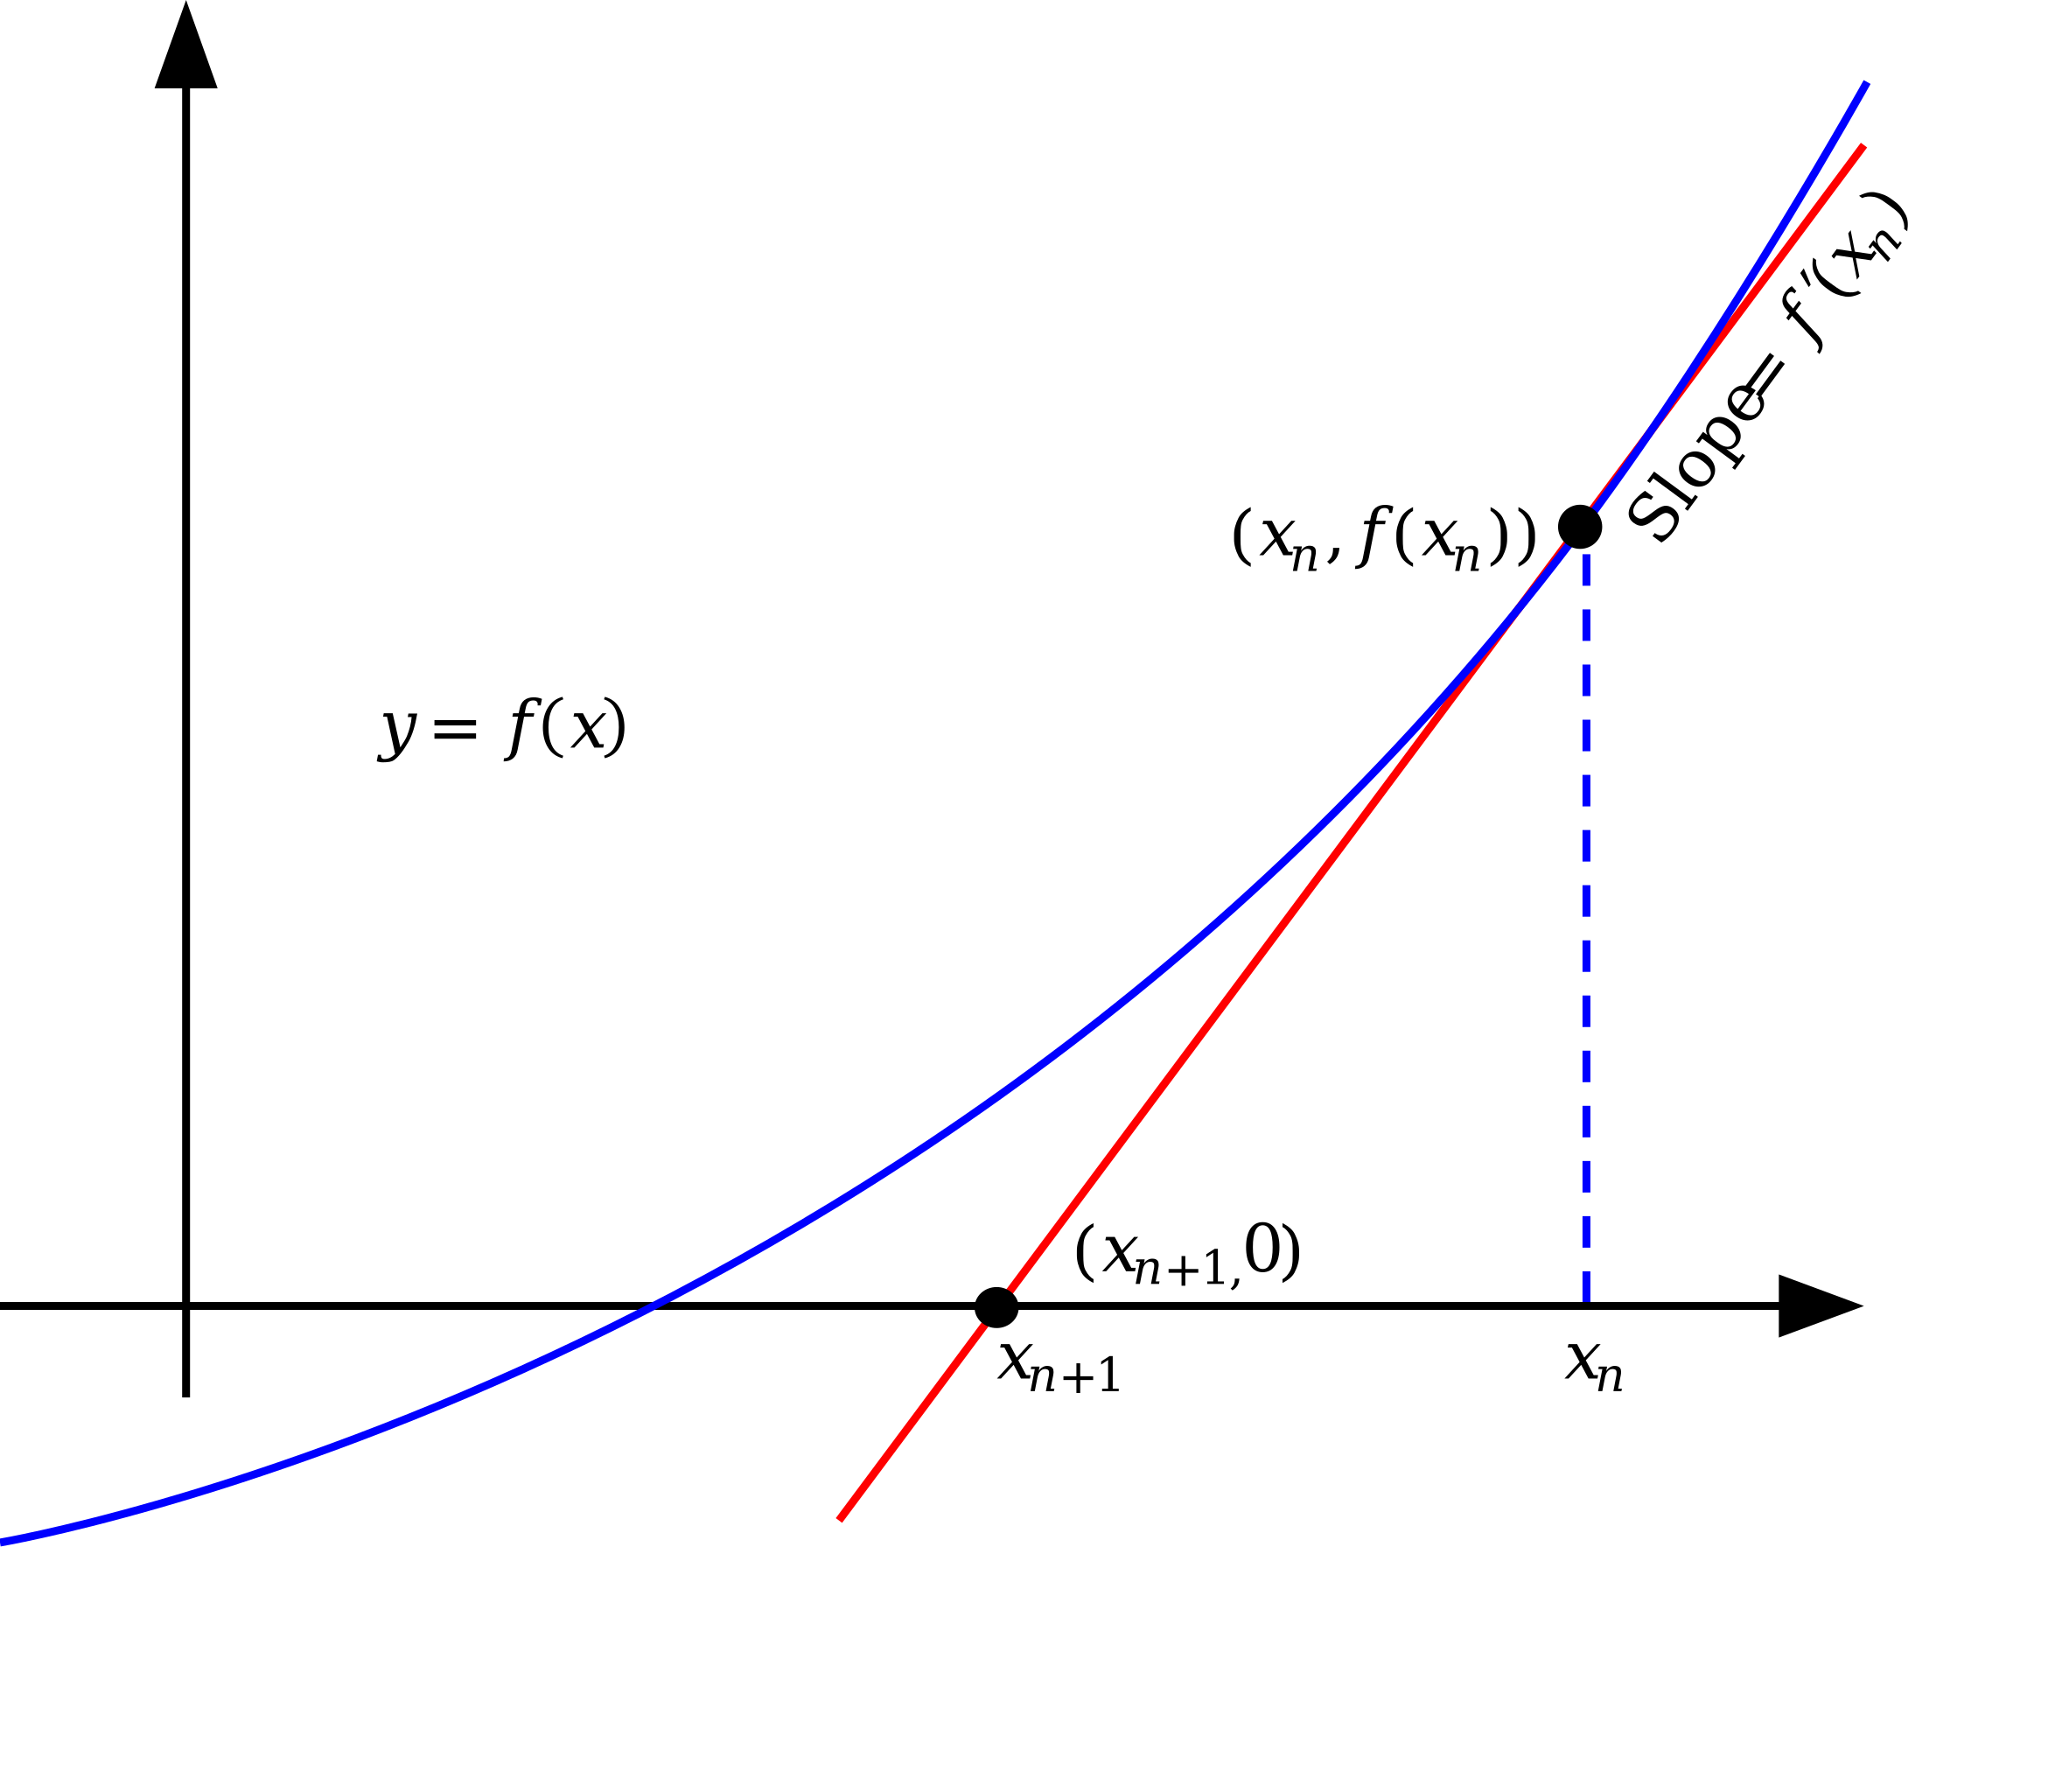
\includegraphics[width=0.5\textwidth, alt ={A schematic of the first step of Newton's method for finding roots}]{figures/Newton_iteration}
    %}{A schematic of a derivative as a tangent to a curve. }
    \caption{The first step of Newton's iteration method to find the root of $f(x)$. We pick a point $x_{0}$ then find the tangent to $f(x)$ at $x_{0}$ and solve for the point $x_{1}$ where this tangent intersects the $x$-axis. This is repeated until we converge on the root.}
\label{fig: Newton iteration}
\end{figure}


For the specific equation in \cref{eq: equation for iterating} we have that
\begin{equation}
x_{n+1}=x_{n}-\frac{x_{n}^{5}-3x_{n}^3+2x_{n}-4}{5x_{n}^{4}-9x_{n}^{2}+2}.
\end{equation}

Starting from $x_{0}=1.8$ we get the sequence in \cref{table:3}. This iteration scheme converges to the precise answer of \cref{eq: precise root} much quicker than the other methods.


Newton's method is the approach that you need to be able to use during this module so we will treat a couple more examples using it. There are a couple more examples on \citep{calcI} if you want to see more.

\begin{ex}
Use Newton's method to determine an approximation to the solution to $\sin{x} = -x$ that lie in the interval $[-1,1]$. Find the approximation to $6$ decimal places.\\

First we need to pick a starting point $x_{0}$. Here we will take $x_{0}=0.5$, you can get an idea of what value to pick by plotting the function. For this example we have that
\begin{equation}
f(x)=\sin(x)+x=0,
\label{eq: sin +x roots}
\end{equation}
so the iteration equation for Newton's method \cref{eq: Newton iteration scheme} becomes
\begin{equation*}
x_{n+1}=x_{n}-\frac{\sin{x_{n}}+x_{n}}{\cos{x_{n}}+1}.
\end{equation*}

The first approximation is then
\begin{equation*}
x_{1}=\frac{1}{2}-\frac{\sin{\frac{1}{2}}+\frac{1}{2}}{\cos{\frac{1}{2}}+1}=-0.0216418
\end{equation*}

\begin{table}[ht]
\centering
\caption{Successive approximations to the root of \cref{eq: sin +x roots} using Newton's method.}

\vspace{2mm}

\label{table:4}



\begin{tabular}{|c|c|c|} 
 \hline
$n$& $x_{n}$ &$f(x_{n})$\\
 \hline
 $0$ & $0.5$ & $0.979426$ \\
 \hline
$1$ &$-0.021642$ & $-0.043282$ \\
\hline
$2$ &$2\times10^{-6}$ & $3.\times10^{-6}$	\\
\hline
$3$ & $0$& $0$\\
\hline
\end{tabular}
\end{table}

The further iteration steps are shown in \cref{table:4}, and we see that to 6 decimal places, it only takes $4$ iterative steps to find that the root is at $x=0$. If we did any more steps we would see that these remain at $x=0$.

\end{ex}

Now we can consider one of the examples from \citep{calcI} which shows when Newton's method does not work.

\begin{ex}
Starting from $x_{0}=1$ we will apply Newton's method to $\sqrt[3]{x}$.\\

Intuitively it is clear that the root is $x=0$. However, Newton's method will not find this root. For this example \cref{eq: Newton iteration scheme} becomes
\begin{equation*}
x_{n+1}=x_{n}-\frac{\sqrt[3]{x}}{\frac{1}{3}x^{-\frac{2}{3}}}=x_{n}-3x_{n}=-2x_{n}.
\end{equation*}

This already tells us that instead of converging to $x=0$, Newton's method will diverge with $x_{1}=-2$, $x_{2}=4$, $x_{3}=-8$, $x_{4}=16$, \dots{}. This is the opposite of what we want. Fortunately, it became obvious quite quickly that the method was not working and we did not have to waste much time before discovering that we needed to used a different model.
\end{ex}

\begin{exercise}
Write a computer program to implement Newton's method and use it to find the roots in the examples above, where Newton's method works.
\end{exercise}

\subsection*{Secant method}
A variant of Newton's method is the \textbf{Secant} method, where we start with two estimates of the root, $x_{0}$ and $x_{1}$ and estimate the derivative as being the Newton quotient
\begin{equation*}
Q(x_{0},x_{1})=\frac{f(x_{1})-f(x_{1})}{x_{1}-x_{0}},
\end{equation*}
so that
\begin{equation*}
x_{2}=x_{1}-\frac{f(x_{1})}{Q(x_{0},x_{1})}=x_{1}-\frac{f(x_{1})}{\frac{f(x_{1})-f(x_{1})}{x_{1}-x_{0}}}.
\end{equation*}

This means that the iteration scheme is given by
\begin{equation}
x_{n+1}=x_{n}-\frac{f(x_{n})}{Q(x_{n-1},x_{n})}=x_{n}-\frac{f(x_{n})}{\frac{f(x_{n})-f(x_{n-1})}{x_{n}-x_{n-1}}}
\label{eq: secant method}
\end{equation}

Geometrically, the secant method can also be viewed as constructing a line nearby our function and moving to the point where this line cuts the $x$-axis. However, this line is no longer a tangent line, but is a secant. 

\begin{ex}
For 
\begin{equation*}
f(x)=x^{2}-10,
\end{equation*}
and taking $x_{0}=2$, $x_{1}=3$ we find $x_{2}$ using the secant method as follows:

\begin{align*}
x_{2}&=x_{1}-\frac{f(x_{1})}{\frac{f(x_{1})-f(x_{0})}{x_{1}-x_{0}}}\\
	&=3-\frac{-1}{\frac{-1-(-6)}{3-2}}\\
	&=3+\frac{1}{7}\\
	&=3.14286.
\end{align*}
This is an equation that we can solve directly by the rearrangement method since $f(x)=0$ corresponds to $x^{2}=10$ so the exact answers are $x=-\sqrt{10}\simeq -3.16228$ and $x=\sqrt{10}\simeq 3.16228$. We can see that $x_{2}$ is already approaching this exact answer.

\end{ex}

\subsection*{Convergence and errors}
The absolute error of a numerical method is the difference between the true solution $x$ and the approximate solution $\xi$, $\epsilon =\vert x-\xi\vert$. It can be hard to estimate the absolute error unless we already know the exact solution. \\

We say that an iteration scheme converges when it subsequent iterations do not change the value of $x_{n}$, at least to the accuracy that we are looking for. Not every method will converge for a given problem, We have already seen that Newton's method does not converge for the cube root, $\sqrt[3]{x}$. You will gain experience of which methods works best for which type of of problem. In this module, you will mainly be using Newton's method so you need to remember that it can fail.

\section{Numerical differentiation}

\section{Numerical integration}

\section{Numerical approaches to differential equations}
\newpage

%%%%%%%%%%%%%%%%%%%%%%%%%%%%%%%%%%%%%%%%%%%%%%

\chapter{Advanced Topics}
\label{sec:advanced topics}
This section is non examinable and is included so that you have a feel for how the material in this module can be taken further.

\section{L'H\^{o}pital's rule for evaluating limits}
\label{sec:l'hopital}
We saw in \cref{sec:functions} that some limits lead to nonsense expressions. For example, If we were confronted with $\lim_{x\to 0}\sin(x)/x$, this looks like it will result in $0/0$ which is does not make sense. Remember that not all limits that look indeterminate really are. For example
\begin{equation*}
\lim_{x\to 4}\frac{x^{2}-16}{x-4}
\end{equation*}
looks at first glance like it will have the form $0/0$ since both the numerator and denominator vanish for $x=4$. However, the numerator can be factored as $x^{2}-16=(x-4)(x+4)$ so the limit simplifies to
\begin{equation*}
\lim_{x\to 4}\frac{x^{2}-16}{x-4}=\lim_{x\to 4}\frac{(x-4)(x+4)}{x-4}=\lim_{x\to4}(x+4)=8.
\end{equation*}
This is why we said that you should try to expand and simplify the function that you are taking the limit of as much as possible. \\

L'H\^{o}pital\footnote{Originally spelt L'Hospital, with a silent s and no circumflex}'s rule enable us to make sense of some of those limits which still look indeterminate after they have been simplified. To apply L'H\^{o}pital's rule, we have to be taking the limit of a ratio of functions $f(x),g(x)$, where both are differentiable, the derivative of $g(x)$ does not vanish, and in the limit $f(x)$ and $g(x)$ wither both go to zero or both go to infinity. Then we have that
\begin{equation}
\lim_{x\to a}\frac{f(x)}{g(x)}=\lim_{x\to a}\frac{f'(x)}{g'(x)},
\label{eq: l'hopital's rule}
\end{equation}
so we can replace the ratio of the functions with the ratio of their derivatives. If both of the derivatives still vanish, or diverge, in the limit, then process can be repeated and we end up with more derivatives
\begin{equation*}
\lim_{x\to a}\frac{f(x)}{g(x)}=\lim_{x\to a}\frac{f^{(n)}(x)}{g^{(n)}(x)},
\end{equation*}
where the superscript $(n)$ means that we are differentiating the functions $n$ times.\\

Note that if the limit does not lead to an indeterminate then L'H\^{o}pital's rule does not hold!

\begin{ex}
As a counter example consider the limit
\begin{equation*}
\lim_{x\to 1}\frac{f(x)}{g(x)}=\lim_{x\to 1}\frac{x+1}{2x+1}.
\end{equation*}
Both $\lim_{x\to 1}f(x)=2$ and $\lim_{x\to1}g(x)=3$ are finite and no-zero. Evaluating the limit directly gives
\begin{equation*}
\lim_{x\to 1}\frac{x+1}{2x+1}=\frac{2}{3}.
\end{equation*}
We can also calculate the limit of the ratio of derivatives,
\begin{equation*}
\lim_{x\to 1}\frac{f'(x)}{g'(x)}\lim_{x\to 1}\frac{1}{2}=\frac{1}{2}\neq \frac{2}{3}.
\end{equation*}
So the limit of the ratio does not match the limit of the ratio of derivatives.
\end{ex}


As long as our original limit looks like it is indeterminate we can use L'H\^{o}pital's rule.

\begin{ex}
The limit of $\sin(x)/x$ as $x\to 0$ is evaluated as follows
\begin{equation*}
\lim_{x\to0}\frac{\sin(x)}{x}=\lim_{x\to0}\frac{\cos(x)}{1}=1.
\end{equation*}
\end{ex}

We can also evaluate other limits that may not at first look like a ratio of functions.
\begin{ex}
Consider the limit $\lim_{x\to-\infty}xe^{x}$ this looks like it becomes the indeterminate $(-\infty)(0)$. If we recall that $1/e^{x}=e^{-x}$ then we can rewrite the limit as
\begin{equation*}
\lim_{x\to-\infty}xe^{x}=\lim_{x\to-\infty}\frac{x}{e^{-x}},
\end{equation*}
which looks like the indeterminate $-\infty/\infty$. Now we can apply L'H\^{o}pital's rule to get
\begin{equation*}
\lim_{x\to-\infty}\frac{x}{e^{-x}}=\lim_{x\to-\infty}\frac{1}{-e^{-x}}=0,
\end{equation*}
since $1/\infty$ is zero.
\end{ex}

\section{Functions of two variables}

\section{Multiple integrals}

\section{Optimisation Problems}

\section{Polynomial approximation}
\newpage

%%%%%%%%%%%%%%%%%%%%%%%%%%%%%%%%%%%%%%%%%%%%%%


\chapter{Background Mathematics}
\label{sec:background}

\epigraph{Try as you may you just can't get away from Mathematics }{\textit{That's Mathematics by Tom Lehrer}}

\section{Background and References}
As this is a maths module there is a lot of assumed background.  This means that to understand the material in the module and to be able to solve the tutorial problems, you need to have a experience with a variety of mathematical techniques such as:
\begin{itemize}
%\setlength{\itemsep}{-5pt}
    \item solving linear equation,
    \item solving quadratic equations
    \item using trigonometry,
    \item knowning some simple functions.
\end{itemize}

These topics will be familiar to many of you. However, it may have been a while since some of you studied mathematics and I am aiming to briefly introduce any new mathematical topics when we need them. However, I also want to link to some extra resources where you can brush up on your maths beforehand.\\


A great resource is the website \href{https://tutorial.math.lamar.edu/}{Pauls Online Math Notes}. The website contains notes for a variety of mathematics courses including algebra and calculus. The most useful background materials are the Algebra and trigonometry review \href{https://tutorial.math.lamar.edu/Extras/AlgebraTrigReview/AlgebraTrigIntro.aspx}{linked here} and the preliminaries section of the algebra notes, \href{https://tutorial.math.lamar.edu/Classes/Alg/Preliminaries.aspx}{linked here}.\\

As the module goes on I may add more background resources or add some examples.\\

%The essential maths skills needed for studying physics at this level are nicely summarised in \citep{garrett2015essential}. It is worth having a look at this book if you want to revise the maths background.

\section{Polynomials and roots}
One of the most common examples of a function that we will meet is a polynomial. These are functions wher ethe variable $x$ is sent to a sum of powers of $x$,
\begin{equation}
p(x)=a_{n}x^{n}+a_{n-1}x^{n-1}\cdots +a_{1}x+a_{0}.
\label{eq: polynomial}
\end{equation}
If we plot a polynomial, e.g. produce the graph $(x,y=p(x))$, then the locations where the plot cuts the $x$-axis, where $y=p(x)=0$, are called the zeros or roots. For a linear equation we solve it via rearrangement, see \cref{sec: rearranging}. For a quadratic equation like
\begin{equation*}
ax^{2}+bx+c=0,
\end{equation*}
we solve it using the quadratic formula
\begin{equation}
x=\frac{-b\pm\sqrt{b^{2}-4ac}}{2a}.
\end{equation}

As an example consider the quadratic equation
\begin{equation*}
2x^{2}-4x-2=0.
\end{equation*}
To apply the quadratic formula we compare this specific equation to the general quadratic equation above, and note that $a=2,b=-4,c=-2$. The quadratic formula thus gives
\begin{align*}
x 	&=\frac{4\pm\sqrt{4^{2}+4\times2\times2}}{4}\\
	&=\frac{4\pm\sqrt{16+16}}{4}\\
	&=1\pm\frac{\sqrt{32}}{4}\\
	&=1\pm\frac{\sqrt{16}\sqrt{2}}{4}\\
	&=1\pm\sqrt{2}.
\end{align*}
So the two roots are $1+\sqrt{2}$, $1-\sqrt{2}$.\\

Note that we can guess the roots by looking at the polynomial. A quadratic can always be written as 
\begin{align*}
a(x-\alpha)(x-\beta)	&=a\left(x^{2}-(\alpha+\beta)x+\alpha\beta\right)\\
				&=ax^{2}-a\left(\alpha+\beta\right)+a\alpha\beta.
\end{align*}
So the product of the roots is related to the constant term, and the sum of the roots is related to the linear term. This means that we can guess one of the roots by looking at the factors of the constant term. For quadratics we do not need to do this, but with higher order equations this is very useful.\\

For higher order polynomials we do not have a formula to find the solutions\footnote{The exception is cubic equations. There is a cubic formula. However, it is fairly complicated and there is no point in trying to use it.} In this case we use the higher order versions of the above identity that the constant term in the polynomial is related to the product of the roots. We can then use a technique like polynomial long division to reduce the order of the equation.\\

Consider the equation
\begin{equation*}
x^{3}+x^{2}-x-1=0
\end{equation*}
Since $(x-a)(x-b)(x-c)$ has a constant term $-abc$ we see that the product of the three roots is $1$. This means that we can guess that $1$ is one of the roots. 

\begin{warpprint}
We can the perform polynomial long division to find that
\begin{equation*}
\polylongdiv{x^3+x^2-x-1}{x-1}
\end{equation*}
This means that we can rewrite
\begin{equation*}
x^{3}+x^{2}-x-1=(x-1)(x^{2}+2x+1),
\end{equation*}
and then we can either factorise the quadratic directly or use the quadratic formula. Note that we could also solve this case using polynomial long division by noting that the product of the roots is $1$ so we can guess that $-1$ is a repeated root and calculate
\begin{equation*}
\polylongdiv{x^{2}+2x+1}{x+1}
\end{equation*}
\end{warpprint}

\begin{warpHTML}
We then need to use polynomial long division to factor out this root and reduce our equation to a quadratic that we can then solve. If you read the pdf version of these notes then it is nice and easy to include examples of polynomial long division. Unfortunately in the HTML version this does not display properly so we need to proceed more slowly.\\

You may remember for your time at school learning about long division, the idea is you want to know how many times a small number goes into a big number. You are likely familiar with a couple of notations for this such as $a\div b$ or $a/b$.  When the number we are dividing, $a$ involves lots of digits it is easier to write it as
\begin{equation*}
b)\overline{a}.
\end{equation*}
Long division is the process of carrying out these calculations.\\

Consider the problem of dividing $1260257$ by 37, this is done as follows
\begin{align*}
& \phantom{++}34061\\
37&)\overline{1260257}\\
&\underline{1110000}\\
&\phantom{1}150257\\
&\phantom{1}\underline{148000}\\
&\phantom{111}2257\\
&\phantom{111}\underline{2220}\\
&\phantom{11111}37
\end{align*}
For understanding the steps I recommend having a look at the Wikipedia article on long division if you want a refresher as it contains lots of examples. The key idea is that you work term by term, typically ignoring the digits on the right, until you have a number that is bigger than your starting one, in this case $37$. Then you write down how many times 37 goes it to that number, in this case $37$ goes into $126$ $3$ times, and $3\times 37=111$, and you proceed onwards like this.\\

For polynomials the process is pretty much the same you write down the polynomial that you were given originally, eg $x^{3}+x^{2}-x-1$, then you write down the linear expression that you want to divide it by, here $x-1$. This means we have the division problem
\begin{align*}
x-1&)\overline{x^{3}+x^{2}-x-1}.
\end{align*}
First we look at the highest order $x$ terms and see that we need to multiply $x-1$ by $x^2$ to get an $x^3$ term so we can write down
\begin{align*}
&\phantom{+}x^{2}\\
x-1&)\overline{x^{3}+x^{2}-x-1}\\
&\phantom{+}\underline{x^{3}-x^{2}}
\end{align*}
We can then subtracted the third line from the second line to get
\begin{align*}
&\phantom{+}x^{2}\\
x-1&)\overline{x^{3}+x^{2}-x-1}\\
&\phantom{+}\underline{x^{3}-x^{2}}\\
&\phantom{++}2x^{2}-x-1
\end{align*}
Now we need to multiply $x-1$ by $2x$ to cancel the highest order term so we have that
\begin{align*}
&\phantom{+}x^{2}+2x\\
x-1&)\overline{x^{3}+x^{2}-x-1}\\
&\phantom{+}\underline{x^{3}-x^{2}}\\
&\phantom{++}2x^{2}-x-1\\
&\phantom{++}\underline{2x^{2}-2x}
\end{align*}
Carrying out the subtraction now gives
\begin{align*}
&\phantom{+}x^{2}+2x\\
x-1&)\overline{x^{3}+x^{2}-x-1}\\
&\phantom{+}\underline{x^{3}-x^{2}}\\
&\phantom{++}2x^{2}-x-1\\
&\phantom{++}\underline{2x^{2}-2x}\\
&\phantom{++++}x-1
\end{align*}
which is exactly what we are dividing by. Thus
\begin{align*}
&\phantom{+}x^{2}+2x+1\\
x-1&)\overline{x^{3}+x^{2}-x-1}\\
&\phantom{+}\underline{x^{3}-x^{2}}\\
&\phantom{++}2x^{2}-x-1\\
&\phantom{++}\underline{2x^{2}-2x}\\
&\phantom{++++}x-1\\
&\phantom{++++}\underline{x-1}\\
&\phantom{++++++}0.
\end{align*}
Then we can either factorise the quadratic directly or use the quadratic formula. Note that we could also solve this case using polynomial long division by noting that the product of the roots is $1$ so we can guess that $-1$ is a repeated root. Which ever way we approach it we get that
\begin{equation*}
x^{2}+2x+1=(x+1)^{2}.
\end{equation*}
\end{warpHTML}

so we have that
\begin{equation*}
x^{3}+x^{2}-x-1=(x-1)(x+1)^{2}.
\end{equation*}

This style of approach can be applied to any polynomial equation. There is a more complete description of polynomials and their roots given in \cite{algI}.

\section{Trigonometry Primer}
Since trigonometric functions come up a lot in this course a review of the basics is included here. If you are not familiar with it you can either check out the links suggested above or ask me to provide more background information.\\

Here we will only discuss trigonometry for right angled triangles, but in the main content of the module we will deal with general trig functions. \textbf{Trigonometry} is an area of mathematics related to the study of triangles and provides a way to compute the lengths and angles in a triangle provided that you now some of them already.

\begin{figure}[ht]
    \centering
   % \pdftooltip{
   \begin{tikzpicture}[scale=2]
  \coordinate [label=left:$\uptheta$] (C) at (-1.5cm,-1.cm);
  \coordinate (A) at (1.5cm,-1.0cm);
  \coordinate [label=above:$\upphi$] (B) at (1.5cm,1.0cm);
  \draw (C) -- node[above] {$a$} (B) -- node[right] {$c$} (A) -- node[below] {$b$} (C);
  \draw (1.25cm,-1.0cm) rectangle (1.5cm,-0.75cm);
  \tkzMarkAngle[size=1cm,color=blue](A,C,B)
  \tkzMarkAngle[size=1cm,color=blue](C,B,A)
\end{tikzpicture}
%}{A right angle triangle with all the angles and sides marked.}
    \caption{A right angle triangle with all the angles and sides marked.}
    \label{fig: Trig definitions}
\end{figure}

The typical mnemonic used to remember trigonometry is \textbf{SOH CAH TOA} which means Sine is opposite over hypotenuse
\begin{equation*}
\sin\uptheta=\frac{c}{a}, \qquad \sin\upphi =\frac{b}{a},
\end{equation*}
Cosine is adjacent divided by hypotenuse
\begin{equation*}
\cos\uptheta=\frac{b}{a}, \qquad \cos\upphi =\frac{c}{a},
\end{equation*}
and Tangent is opposite divided by adjacent
\begin{equation*}
\tan\uptheta=\frac{c}{b}, \qquad \sin\upphi =\frac{b}{c}.
\end{equation*}
There are associated inverse functions $\arcsin,\arccos,\arctan$ which convert ratios of sides into angles. All of these functions are available on your calculator. \\

It is important to be careful with which units you are using to express angles. It is likely that you will have come across degrees where going around a full circle is represented by an angle of $360^{\circ}$. However, it is often convenient to work with a different measure of angles called radians, in this case we take a full circle to be $2\uppi\text{rad}$ and express angles as a number between $0$ and $2\uppi$. In this module you need to work in radians as otherwise the derivative expressions for trig functions will become more complicated. If you are unfamiliar with  radians have a look at the next section which explains more about them and how to convert between degrees and radians.

\section{Radians and Degrees}
To work with trig functions  we need to know how to describe angles, eg how round in a circle we have gone. Often when working with circles we do not describe angles in terms of degrees but instead use units called radians.  You are likely to be familiar with describing angles in a degrees where a full rotation is $360^{\circ}$ and a half rotation is $180^{\circ}$. \textbf{Radians} are an alternative, and some would say ``better'' method of measuring angles, the certainly simplify some computations, though they can seem confusing when we first meet them.\\

The basic idea of radians is to work in terms of the distance around the circle that the angle corresponds to.  For a circle with radius $r$ the circumference is $c=2\uppi r$, while an arc of the circle would have length s, shown in red in \cref{fig: radians}. Radians are defined in terms of the length of arcs as
\begin{equation}
\ut =\frac{s}{r},
\label{eq: definition of radians}
\end{equation}
in other words, an angle measured in radians is the ratio of the distance travelled on an arc round the circle to the radius of the circle. 
This means that a full rotation $360^{\circ}$ corresponds to $2\uppi$ radians as in this case $s=2\uppi r$, half a rotation or $180^{\circ}$ then corresponds to $\uppi$ radians. 

\begin{figure}[ht]
    \centering
 %   \pdftooltip{
    \begin{tikzpicture}
   % \draw[step=1cm,gray,very thin] (3,-3) grid (3,3);
   \filldraw[color = blue, ultra thick](0,0) circle (0.05);
    \draw[ ultra thick](0,0) circle (2);
    \draw[ultra thick] (0,0) -- (1.414,1.414);
  \node[anchor =south] at (0.7,0.7) {$r$};
    \draw[ultra thick] (0,0) -- (2,0);
    \draw[ultra thick] (1,0) arc (0:45:1) node[anchor=north]{$\ut$};
     \draw[ultra thick, color=red] (2,0) arc (0:45:2) node[anchor=north]{$s$};
    \end{tikzpicture}
  %  }{A circle}
    \caption{A circle of radius $r$ showing how arc length around the circle corresponds to angles}
        \label{fig: radians}
\end{figure}

More generally the conversion rule is that
\begin{equation*}
\text{radians} = \frac{180^{\circ}}{\uppi}\times \text{degrees}.
\end{equation*}
The main advantage of radians comes when differentiating and expanding functions as working in degrees requires extra terms to be included and greater care to be taken. While we will not be doing any differentiation in this module we will come across some expressions where we need to work in radians for the quoted expressions to be valid. When this happens we will include a warning so that it is clear where you need to be careful.\\

One way to motivate working in radians is to think of unwinding the circle to get a straight line, for a circle of radius $r$ this length will be the circumference, if we divide this length by $r$ we will have a line if length $2\uppi$ and the angle in radians will be the distance travelled along this line. In other words, working in radians is a bit like converting from circular motion to linear motion.

\begin{figure}[ht]
    \centering
  %  \pdftooltip{
    \begin{tikzpicture}
   % \draw[step=1cm,gray,very thin] (3,-3) grid (3,3);
   \filldraw[color = blue, ultra thick](0,0) circle (0.05);
    \draw[ ultra thick](0,0) circle (2);
    \draw[ultra thick] (0,0) -- (1.414,1.414);
 % \node[anchor =south] at (0.7,0.7) {$r$};
    \draw[ultra thick] (0,0) -- (2,0);
    \draw[ultra thick] (1,0) arc (0:45:1) node[anchor=north]{$\ut$};
     \draw[ultra thick, color=red] (2,0) arc (0:45:2) node[anchor=north]{$s$};
     \draw[ultra thick] (6,-3.14) --(6,3.14);
     \draw[ultra thick, color = red] (6,-3.14) --(6,-2.355) node[anchor=west]{$\ut$};
     \draw[ultra thick, ->] (2.5,0) -- (5.5,0);
    \end{tikzpicture}
  %  }{A circle}
    \caption{A circle of radius $r$ showing how arc length around the circle corresponds to angles}
        \label{fig: radians 2}
\end{figure}

As evidenced in \cref{fig: radians,fig: radians 2}, it is common practice to use the Greek letter theta, $\ut$, to denote an angle. Other Greek letters like phi, $\upphi$ or $\upvarphi$, and psi, $\uppsi$, are sometimes used as well. It is worth spending some time familiarising yourself with these Greek letters so you do not think that they are just badly written English letters.

\section{Rearranging Equations}
\label{sec: rearranging}
A very important skill for solving mathematics problems, and finding the roots of functions, is to be able to rearrange equations. This is sometimes referred to as changing the subject of an equation. Newcastle University have a webpage, available \href{https://www.mas.ncl.ac.uk/ask/numeracy-maths-statistics/core-mathematics/pure-maths/algebra/rearranging-equations.html}{here} that goes through some examples of how to rearrange equations. The webpage also has some self test questions that you can look at if you want more practice. Some of the details are reviewed here, along with examples for the specific equations that we have been using in this module.\\


In the equation
\begin{equation*}
x=5y+4z,
\end{equation*}
$x$ is called the subject, which is just a fancy way of saying that $x$ is expressed in terms of the other variables. When we talk about rearranging an equation, we mean that we change the subject of the equation from $x$ to another variable like $y$ and $z$. We do this by performing a variety of mathematical operations to both sides of the equation to swap some of the variables from one side to the other. \\

These operations can include: adding or subtracting a quantity from both sides, multiplying or dividing by a quantity, taking logarithms of or exponentiating both sides of the equation, raising both sides of the equation to any non-zero power.\\
\begin{ex}
Returning to the above equation $x=5y+4x$, we can rearrange it to make $z$ the subject. Again, this means that we will perform mathematical operations on both sides of the equation to put it in the form $z=\dots{}$ : 
\begin{align*}
x&=5y+4z, \quad \text{ first subtract $5y$ from both sides},\\
x-5y&=5y+4z-5y=4z, \quad \text{then divide both sides by 4},\\
\frac{x-5y}{4}&=\frac{4z}{4}=z.
\end{align*}
This gives us
\begin{equation*}
z=\frac{x-5y}{4},
\end{equation*}
with $z$ now the subject of the equation.
\end{ex}

\begin{ex}
As another example consider an equation from physics $v=u+at$, which says that the if an object starts off with a velocity $v$ and accelerates at a rate $a$ then after time $t$ its velocity will be $v$. Here we go through this step by step what we do when solving for $a$:
\begin{align*}
v&=u+at, \quad \text{subtract $u$ from both sides},\\
v-u&=u+at -u=at, \quad \text{divide both sides by $t$},\\
\frac{v-u}{t}&=\frac{at}{t}=a,
\end{align*}
which gives us
\begin{equation*}
a=\frac{v-u}{t}.
\end{equation*}
\end{ex}

\begin{ex}
Another example is rearranging a different equation from physics,
\begin{equation*}
s=ut+\frac{1}{2}at^{2},
\end{equation*}
to solve for either $a$ or $t$.\\

To make $a$ the subject we proceed as follows:
\begin{align*}
s&=ut+\frac{1}{2}at^{2}, \quad \text{subtract $ut$ from both sides},\\
s-ut&=ut+\frac{1}{2}at^{2}-ut=\frac{1}{2}at^{2}, \quad \text{multiply both sides by $2$},\\
2\left(s-ut\right)&=2\left(\frac{1}{2}at^{2}\right)=at^{2}, \quad \text{divide both sides by $t^{2}$},\\
\frac{2\left(s-ut\right)}{t^{2}}&=\frac{at^{2}}{t^{2}}=a,
\end{align*}
thus the equation with $a$ being the subject is 
\begin{equation*}
a=\frac{2\left(s-ut\right)}{t^{2}}.
\end{equation*}

If instead we wanted $t$ to be the subject then it is easier to put it in the form of a quadratic equation and then use the quadratic formula:
\begin{align*}
s&=ut+\frac{1}{2}at^{2}, \quad \text{subtract $s$ from both sides},\\
0&=\frac{1}{2}at^{2}+ut-s,\quad \text{this is a qudratic equation for $t$ and is solved by}\\
t&=\frac{-u\pm\sqrt{u^{2}+2as}}{a}.
\end{align*}
\end{ex}

There are a few special cases where we do not need to use the quadratic formula that it is worth being aware of. If $s=0$ then we have
\begin{align*}
0&=ut+\frac{1}{2}at^{2}, \quad \text{factor out the common factor},\\
0&=t\left(u+\frac{1}{2}at\right),
\end{align*}
This has two solutions $t=0$, which is the start of the motion, and
\begin{align*}
0&=u+\frac{1}{2}at, \quad \text{subtract $u$ from both sides},\\
-u&=\frac{1}{2}at, \quad \text{multiply both sides by $2$},\\
-2u&=at, \quad \text{divide both sides by $a$},\\
-\frac{2u}{a}&=t.
\end{align*}
This case often appear when considering projectile motion and you want to calculate the total length of time that the projectile is in the air for.\\

The other common example is if $u=0$, then:
\begin{align*}
s&=\frac{1}{2}at^{2}, \quad \text{multiply both sides by $2$},\\
2s&=at^{2}, \quad \text{divide both sides by $a$},\\
\frac{2s}{a}&=t^{2}, \quad \text{take the square root of both sides},\\
\sqrt{\frac{2s}{a}}&=t.
\end{align*}
In the last line we have dropped the $\pm$ that should be in front of the square root since we do not consider negative time. However, if you were just solving a quadratic equation then you would have to remember to include that.  Both of these special cases can also be found by direct substitution into the quadratic formula of $s=0$ or $u=0$ respectively.\\

\begin{ex}
The final example is to rearrange an equation involving a square root,
\begin{equation*}
T=2\uppi\sqrt{\frac{l}{g}}.
\end{equation*}
If you are asked to make $l$ the subject of this equation we proceed as follows:
\begin{align*}
T&=2\uppi\sqrt{\frac{l}{g}}, \quad \text{first divide both sides by $2\uppi$},\\
\frac{T}{2\uppi}&=\frac{2\uppi}{2\uppi}\sqrt{\frac{l}{g}}=\sqrt{\frac{l}{g}}, \quad \text{then square both sides of the equation},\\
\left(\frac{T}{2\uppi}\right)^{2}&=\left(\sqrt{\frac{l}{g}}\right)^{2}=\frac{l}{g}, \quad \text{now multiply both sides by $g$},\\
g\left(\frac{T}{2\uppi}\right)^{2}&=g\times\frac{l}{g}=l.
\end{align*}
This leaves us with
\begin{equation*}
l=g\left(\frac{T}{2\uppi}\right)^{2}=\frac{gT^{2}}{4\uppi^{2}}.
\end{equation*}
This is the equation for a straight line $y=mx+c$ where $l$ plays the role of $y$, the $y$-intercept $c=0$, $\left(\frac{T}{2\uppi}\right)^{2}$ plays the role of $x$, and $m=g$ is the gradient of the straight line. When analysing your data you would use plot your data and should observe a straight line whose gradient is $g$.\\

At the last step of this rearrangement we could instead make $g$ the subject. To do this we proceed as follows:
\begin{align*}
\left(\frac{T}{2\uppi}\right)^{2}&=\left(\sqrt{\frac{l}{g}}\right)^{2}=\frac{l}{g}, \quad \text{now multiply both sides by $g$},\\
g\left(\frac{T}{2\uppi}\right)^{2}&=g\times \frac{l}{g}=l, \quad \text{divide both sides by }\left(\frac{T}{2\uppi}\right)^{2}, \\
g&=\frac{l}{\left(\frac{T}{2\uppi}\right)^{2}}=\frac{4\uppi^{2} l}{T^{2}}.
\end{align*}
\end{ex}

If you want more examples there is a \textbf{Transposition of Formulae} workbook, designed by mathcentre,  available \href{https://www.mathcentre.ac.uk/resources/uploaded/mc-ty-transposition-2009-1.pdf}{here}.


\newpage

%%%%%%%%%%%%%%%%%%%%%%%%%%%%%%%%%%%%%%%%%%%%%%

\chapter{Further Reading}
\label{sec:further reading}

\epigraph{Mathematics, you see, is not a spectator sport. To understand mathematics means to be able to do mathematics. And what does it mean doing mathematics? In the first place, it means to be able to solve mathematical problems. }{\textit{How to Solve It by George P\'{o}lya}}

What we discuss in the lectures is just a guide to calculus its many uses. Depending on the modules that you take later on in your degree you will meet Calculus in different guises, particularly when you come across optimisation problems . In this section I will provide links to further resources and suggestions for further reading based on the material that we met each week. If you have any questions about the topics linked here or you want to get even more information then drop me an \href{mailto:rossc@edgehill.ac.uk}{email}.\\

It is important to remember that the lectures are their to introduce you to topics and signpost where to find out more information. If you are just attending the lectures and not doing any further reading or solving practice problems then you will struggle to pass the course. Each 20 credit module is considered 200 hours of work, only 36 hours of which are the lectures and seminars. You are expected to put in around 164 hours of self study during a 12 week module. The resources linked here will help with this self study.\\

\section{Why Calculus Extra Reading}
MIT have a course called \textbf{Calculus for Beginners and Artists} which contains some overlap with this module.  The webpage for the course is available \href{https://math.mit.edu/~djk/calculus_beginners/index.html}{here} and some sections of it, particularly \textbf{Chapter 0: Why Study Calculus?} are worth a read to complement what we will do in this module. I will occasionally suggest reading sections of these notes or sections of \citep{calcI} for a complementary explanation. 



\section{Functions Extra Reading}


\section{Differentiation Extra Reading}
The main reference for this section and many of the other sections of these lecture notes is the wonderful book \textbf{Mathematical Methods for Physics and Engineering}, \citep{riley_mathematical_2006}. There are several copies of this book and its student solution manual in the library and I recommend that you try and have a look at this at some stage.\\

\section{Integration Extra Reading}

\section{Differential Equations Extra Reading}

\section{Numerical Methods Extra Reading}

\section{Advanced Topics Extra Reading}

\newpage

%%%%%%%%%%%%%%%%%%%%%%%%%%%%%%%%%%%%%%%%%%%%%%

\chapter{Tutorial Sheets}
\label{sec: tutorial sheets}

Here we collect all of the tutorial problems for the module. They are split into different weeks depending on the topic they relate to and when they were given out.\\

Many of these questions are taken from or adapted from the recommended  books for the module or from some of the linked resources. These problems are to be attempted in the tutorial sessions and are there to help you familiarise yourself with the material that we have covered in the lectures.\\

Problems marked with a star, $(\star)$ are particularly worth attempting. Problems marked with a dagger, $(\dagger)$, are more challenging and often go beyond what we directly discussed in the lectures.\\

The challenge problem sections contain extra problems. Some of them are just there for extra practice, but others are significantly more difficult than what you need to be able to solve to pass the module. If you are finding the content too easy then have a go at the challenge problems. Sometime the challenge problems from one week will be quite similar to the ordinary problems of the next week. as the problems will become more accessible the more material that we cover.

\section{Week 1}
\label{sec: Tutorial sheet 1}
\paragraph{Functions}

\begin{problem}[$\star$]
Find the roots of the polynomial
\begin{equation*}
g(x)=x^2-2x-12
\end{equation*}
and plot the function.
\end{problem}

\begin{problem}
Find the roots of the polynomial
\begin{equation*}
g(x)=x^3+x^2-x-1
\end{equation*}
and plot the function.
\end{problem}

\begin{problem}[$\star$]
Consider the function
\begin{equation*}
g(x)=x^2+2x+2,
\end{equation*}
produce a plot of the function by calculating its value at a selection of points. What do you notice as $x$ gets very large? What happens for $x=0$?
\end{problem}

\begin{problem}[$\star$]
Consider the function
\begin{equation*}
g(x)=\frac{1}{x-4},
\end{equation*}
and plot the function.what happens as $x$ gets large? What happens as $x$ approaches $4$?\\

Plot the function and comment on its behaviour.
\end{problem}

\begin{problem}
Draw a schematic of a one-to-one function between the sets
\begin{equation*}
\begin{split}
&\left\{1,2,3,4,5\right\}\\
&\left\{a,b,c,d,e,f,g\right\}.
\end{split}
\end{equation*}
Is there only one way to do this?
\end{problem}




\begin{problem}[$\star$]
Given the function
\begin{equation*}
f(x)=x^3-2x^2-x+2
\end{equation*}
find:
\begin{itemize}
    \item $f(0)$,
    \item $f(1)$,
    \item $f(-1)$,
    \item $f(2)$,
    \item $f(-2)$,
    \item $f(t)$,
    \item $f(x-1)$.
\end{itemize}
\end{problem}

\begin{problem}
Consider the function
\begin{equation*}
h(x)=\frac{x}{\sqrt{x^{2}-9}}.
\end{equation*}
Find the points where the denominator vanishes, then plot the function avoiding these points. What happens to the plot as the function approaches these points?
\end{problem}


\begin{problem}
Given the functions
\begin{align*}
f(x)&=x^2-x+1,\\
g(x)&=2-x,
\end{align*}
find:
\begin{itemize}
\item $\left(f\circ g\right)(2)$,
\item $\left(g\circ f\right)(2)$,
\item $\left(f\circ g\right)(x)$,
\item $\left(g\circ f\right)(x)$.
\end{itemize}
\end{problem}


\begin{problem}[$\star$]
Given the functions
\begin{align*}
f(x)&=3x-2\\
g(x)&=\frac{x}{3}+\frac{2}{3},
\end{align*}
find:
\begin{itemize}
\item $\left(f\circ g\right)(x)$,
\item $\left(g\circ f\right)(x)$,
\item What is the relationship between $f(x)$ and $g(x)$?
\end{itemize}
\end{problem}


\begin{problem}[$\dagger$]
Given the function
\begin{equation*}
h(x)=\frac{x+4}{2x-5},
\end{equation*}
identify when it has an inverse and calculate the inverse.
\end{problem}

\paragraph{Challenge Problems}

\begin{problem}
Consider the function 
\begin{equation*}
f(x)=\frac{x^{2}-x-12}{x-1}.
\end{equation*}
Identify the points where the numerator and denominator vanish. Plot the function and explain what happens to the function near these points.
\end{problem}

\begin{problem}
Given the function 
\begin{equation*}
f(x)=2x-3,
\end{equation*}
find the inverse function $f^{-1}(x)$.
\end{problem}


\begin{problem}[$\dagger\dagger$]
Build a schematic of a bijection between the natural numbers
\begin{equation*}
\N=\{1,2,3,4,5,\dots\},
\end{equation*}
and the integers
\begin{equation*}
\Z=\{0,1,-1,2,-2,3,-3,\dots\}.
\end{equation*}

Are there more integers than natural numbers?\\

Could you do the same for the real numbers $\R$? If you find this interesting you may want to explore the work of Cantor.
\end{problem}




\section{Week 2}
\label{sec: Tutorial sheet 2}

\paragraph{Polynomials}[$\star$]
\begin{problem}
For the polynomial equation
\begin{equation*}
x^{3}-3x+2=0,
\end{equation*}
express it as a product of its factors.\\

Hint: this means write it as 
\begin{equation*}
\left(x-a\right)\left(x-b\right)\left(x-c\right),
\end{equation*}
where $a,b,c$ are the roots of the polynomial.
\end{problem}

\begin{problem}
Find the roots of the following polynomial equation
\begin{equation*}
x^{4}-4x^{3}+6x^{2}-4x+1=0.
\end{equation*}
\end{problem}

\paragraph{Trig functions}
Remember to work in radians for any problems related to trigonometry.

\begin{problem}
Find the solutions to 
\begin{equation*}
\sqrt{2}\cos x =1.
\end{equation*}
\end{problem}

\begin{problem}
Identify any solutions to the equation
\begin{equation*}
\sin(2x)=-2.
\end{equation*}
\end{problem}

\begin{problem}[$\star$]
Solve
\begin{equation*}
2x\sin x = x.
\end{equation*}
\end{problem}

\paragraph{Exponentials and Logarithms}
\begin{problem}[$\star$]
Solve the equation
\begin{equation*}
x=xe^{4x}.
\end{equation*}
\end{problem}

\begin{problem}[$\star$]
Solve
\begin{equation*}
2\ln x -\ln(x+2)=1.
\end{equation*}
\end{problem}

\paragraph{Limits and Asymptotes}
\begin{problem}[$\star$]
For the function
\begin{equation*}
f(x)=\frac{x^{2}+4x+12}{x^{2}-2x}
\end{equation*}
evaluate the limit
\begin{equation*}
\lim_{x\to 2}f(x).
\end{equation*}
\end{problem}

\begin{problem}[$\star$]
For the function
\begin{equation*}
g(x)=\frac{2x^{4}-x^{2}+8x}{7-5x^{4}}
\end{equation*}
evaluate the limits
\begin{align*}
&\lim_{x\to -\infty}g(x),\\
&\lim_{x\to \infty}g(x).
\end{align*}
\end{problem}

\begin{problem}[$\dagger$]
For the function
\begin{equation*}
h(x)=\frac{6e^{4x}-e^{-2x}}{8e^{4x}-2e^{2x}+3e^{-x}}
\end{equation*}
evaluate the limit
\begin{align*}
&\lim_{x\to \infty}h(x).
\end{align*}
\end{problem}

\begin{problem}
Using an appropriate plot evaluate the limits
\begin{align*}
&\lim_{x\to \frac{\pi}{2}}\tan x,\\
&\lim_{x\to 0}\tan x.
\end{align*}
\end{problem}

\begin{problem}[$\star$]
Determine where the function
\begin{equation*}
g(x)=\frac{x^{3}+x^{2}-x-1}{x^{3}-2x^{2}-4x+8}
\end{equation*}
fails to be continuous. What do these points correspond to on a plot of $g(x)$?
\end{problem}

\paragraph{Challenge Problems}
\begin{problem}
By making a table of values of $f(x), x$ estimate the limit
\begin{equation*}
\lim_{x\to 2}f(x)
\end{equation*}
from above and below for the function
\begin{equation*}
f(x)=\frac{x^{2}+4x-12}{x^{2}-2x}.
\end{equation*}
\end{problem}

\begin{problem}
Use the definition of continuity to determine in the function
\begin{equation*}
g(x)=\frac{4x+10}{x^{2}-2x-15}
\end{equation*}
is continuous and if not find the points where it has discontinuities.
\end{problem}


\begin{problem}[$\dagger$]
For the function $g(x)$ in the previous problem look at the definition of differentiability and work out where $g(x)$ fails to be differentiable.
\end{problem}

\paragraph{Hyperbolic Trig functions}
\begin{problem}[$\dagger$]
Show that
\begin{equation*}
\sinh(x+y)=\sinh x \cosh y+\cosh x \sinh y.
\end{equation*}
\end{problem}

\begin{problem}[$\dagger$]
Following some of the examples in \cref{sec: hyperbolic functions} show that 
\begin{equation*}
\cosh^{-1}x=\ln\left(x\pm\sqrt{x^{2}+1}\right).
\end{equation*}
\end{problem}

\section{Week 3}
\label{sec: Tutorial sheet 3}
\paragraph{Differentiation}

\begin{problem}[$\star$]
Find the derivative of 
\begin{equation*}
f(x)=7x^{2}
\end{equation*}
\begin{itemize}
\item[a)] using first principles,
\item[b)] using the rule for differentiating monomials.
\end{itemize}
\end{problem}

\begin{problem}
Find the derivative of 
\begin{equation*}
f(x)=3x^{3}-8x.
\end{equation*}
\end{problem}



\paragraph{Challenge Problems}





\newpage

%%%%%%%%%%%%%%%%%%%%%%%%%%%%%%%%%%%%%%%%%%%%%%

\chapter{Extra Proofs and Derivations}
\label{sec: proofs}
The material in this chapter is not examinable and is included for completeness. Here we will give a selection of proof and derivations for results and formulas that were used in the rest of the notes. You could consider this whole chapter to be one big mathematical deviation.

To prove the product rule from first principles we proceed as follows. Consider $f(x)=p(x)q(x)$ then
\begin{align*}
\frac{\ud f}{\ud x}		&=\lim_{h\to 0}\frac{f(x+h)-f(x)}{h}\\
				&=\lim_{h\to 0}\frac{p(x+h)q(x+h)-p(x)q(x)}{h}\\
				&=\lim_{h\to 0}\frac{p(x+h)q(x+h)-p(x+h)q(x)+p(x+h)q(x)-p(x)q(x)}{h}\\
				&=\lim_{h\to0}\frac{p(x+h)\left(q(x+h)-g(x)\right)}{h}+\lim_{h\to 0}\frac{\left(p(x+h)-p(x)\right)q(x)}{h}\\
				&=\lim_{h\to 0}p(x+h)\frac{q(x+h)-q(x)}{h}+q(x)\lim_{h\to 0}\frac{p(x+h)-p(x)}{h}\\
				&=p(x)\lim_{h\to 0}\frac{q(x+h)-q(x)}{h}+q(x)\lim_{h\to 0}\frac{p(x+h)-p(x)}{h}\\
				&=p(x)\frac{\ud q}{\ud x}+q(x)\frac{\ud p}{\ud x},
\end{align*}
which is the product rule.\\

For the quotient rule, we can either prove it from first principles, which is fiddly, or we can use the product rule on $f(x)=p(x)g(x)$ where $g(x)=1/q(x)$.  Here we will take the second approach as hopefully that will be easier to follow.  Consider $f(x)=p(x)/q(x)$ and let $g(x)=1/q(x)$ then applying the product rule means that
\begin{align*}
\frac{\ud f}{\ud x}		&=\frac{\ud }{\ud x}\left(p(x)g(x)\right)\\
				&=p(x)\frac{\ud g}{\ud x}+g(x)\frac{\ud p}{\ud x}\\
				&=p(x)\frac{\ud}{\ud x}\left(q^{-1}\right)+\frac{1}{q(x)}\frac{\ud p}{\ud x}\\
				&=-p(x)q^{-2}\frac{\ud q}{\ud x}+\frac{1}{q(x)}\frac{\ud p}{\ud x}\\
				&=\frac{1}{q^{2}}\left(q(x)\frac{\ud p}{\ud x}-p(x)\frac{\ud q}{\ud x}\right).
\end{align*}

\begin{mdiv}
Note that in the above calculation we have used the chain rule, $\left((f\circ g)(x)\right)'=f'(g(x))g'(x)$, which we did not discuss until after we had introduced the quotient rule.  Also, note that if we were mathematicians we would need to carefully think about when $p(x)/q(x)$ is differentiable, and implementing the product rule does not need that, it just gives that $p(x)(q(x))^{-1}$ is differentiable if $p(x)$ and $(q(x))^{-1}$ is.  This is why for mathematicians, they would prove the quotient rule using differentiation from first principles, or using logarithmic differentiation. The interested reader should have a look at the Proof of various derivative properties section of \citep{calcI} to see the proof in this way.
\end{mdiv}

Next, following \citep{calcI}, we prove the chain rule as follows: let $y=f(u), u=g(x)$ then we know that
\begin{equation*}
\frac{\ud u}{\ud x}=\lim_{h\to 0}\frac{u(x+h)-u(x)}{h},
\end{equation*}
and that 
\begin{equation*}
\lim_{h\to 0}\left(\frac{u(x+h)-u(x)}{h}-\frac{\ud u}{\ud x}\right)=\lim_{h\to 0}\frac{u(x+h)-u(x)}{h}-\lim_{h\to 0}\frac{\ud u}{\ud x}=\frac{\ud u}{\ud x}-\frac{\ud u}{\ud x}=0.,
\end{equation*}
Now we can define
\begin{equation*}
v(h)=\begin{cases}
\frac{u(x+h)-u(x)}{h}-\frac{\ud u}{\ud x} \quad \text{if } h\neq 0\\
0 \quad \text{if } h=0
\end{cases}
\end{equation*}
which is continuous at $h=0$ since $\lim_{h\to 0}v(h)=0=v(0)$. \dots{}

\newpage

%%%%%%%%%%%%%%%%%%%%%%%%%%%%%%%%%%%%%%%%%%%%%%


\chapter{Standard Derivatives and Integrals}
\label{sec: deriv sheet}

There are several functions that it is worth knowing the derivatives and integrals of. When we first introduced their derivatives we either derived them from first principles or used techniques like the product rule, chain rule, or integration by parts, to derive them from already known results. However, this takes time. You do not need to memorise the following list of standard derivatives and integrals, but you may find the list to be a useful resource when going through the tutorial problems or when revising for the exam. \\

Remember, you should still be able to derive these results if you need to, the list is just intended as an aid.

\section{Derivatives}

\begin{table}[ht]
\centering

\ThisAltText{A table of standard derivatives.}

\caption{Table of standard derivatives}

\vspace{2mm}

\label{table: derivatives}

\begin{tabular}{|c|c|} 
 \hline
$y=f(x)$ & $\frac{\ud y}{\ud x}=f^{\prime}(x) $\\
 \hline
$n$ constant & $0$  \\
 \hline
$x$ &$1$  \\
\hline
$x^{n}$, $n$ constant &	$nx^{n-1}$	\\
\hline
$e^{kx}$, $k$ constant &	$ke^{kx}$	\\
\hline
$\ln(x)$ &	$\frac{1}{x}$ 	\\
\hline
$\sin(k x)$ &	$k\cos(k x)$ 	\\
\hline
$\cos(kx)$ &	$-k\sin(kx)$\\
\hline
$\tan(kx)$ &	$k\sec^{2}(kx)$	\\
\hline
$\arcsin(x)$ &	$\frac{1}{\sqrt{1-x^{2}}} $	\\
\hline
$\arccos(x)$ & $-\frac{1}{\sqrt{1-x^{2}}}$ \\
\hline
$\sinh(x)$& $\cosh(x)$\\
\hline
$\cosh(x)$ & $\sinh(x)$\\
\hline
$\tanh(x)$ & $\sech^{2}(x)$\\
\hline
$f(x)g(x)$ & $f^{\prime}(x)g(x)+f(x)f^{\prime}(x)$\\
\hline
$\frac{f(x)}{g(x)}$ & $\frac{f^{\prime}(x)g(x)-f(x)f^{\prime}(x)}{(g(x))^{2}} $\\
\hline
\end{tabular}
\end{table}


\section{Integrals}

\begin{table}[ht]
\centering

\ThisAltText{A table of standard derivatives.}

\caption{Table of standard integrals}

\vspace{2mm}

\label{table: integrals}

\begin{tabular}{|c|c|} 
 \hline
$y=f(x)$ & $\int f(x) \ud x$\\
 \hline
 constant $k$ & $kx+c$  \\
 \hline
$x^{n}$ &$\frac{x^{n+1}}{n+1}+c$  \\
\hline
$\frac{1}{x}$ &	$\ln(\vert x\vert )+c$	\\
\hline
$e^{kx}$, $k$ constant &	$\frac{e^{kx}}{k} +c$	\\
\hline
$x^{-n}$ &	$\frac{x^{-n+1}}{-n+1} +c$, $n\neq 1$ 	\\
\hline
$\cos(x)$ & $\sin(x) +c$\\
\hline
$\sin(x)$ & $-\cos(x)+c$\\
\hline
$f(x)g^{\prime}(x)$& $f(x)g(x)-\int f^{\prime}(x)g(x)\ud x $\\
\hline
\end{tabular}
\end{table}

%\newpage

%%%%%%%%%%%%%%%%%%%%%%%%%%%%%%%%%%%%%%%%%%%%%%
\clearpage

\ForceHTMLPage

\begin{warpprint}
\printglossaries
\end{warpprint}

\bibliographystyle{unsrtnat}
\bibliography{physics}

%\begin{warpprint} % For print output ...
%\cleardoublepage % ... a common method to place index entry into TOC.
%\phantomsection
%\addcontentsline{toc}{chapter}{\indexname}
%\end{warpprint}
%\ForceHTMLPage % HTML index will be on its own page.
%\ForceHTMLTOC % HTML index will have its own toc entry.
%\printindex
\end{document}